% ~~~~~~~~~~~~~~~~~~~~~~~~~~~~~~~~~~~~
% EXAMPLE SIMULATION EXPERIMENT
% ~~~~~~~~~~~~~~~~~~~~~~~~~~~~~~~~~~~~
\section{Example simulation experiment (\texttt{L1V3\_repressilator.omex})}
\label{example:repressilator}
This example lists the SED-ML for the example in the introduction (Section~\ref{motivation:example}).  \changed{It illustrates the use of a \element{dimensionTerm} to calculate the maximum value of a vector with the KiSAO term for 'maximum' (\val{KISAO:0000828}) as the \element{term}.  This document can be found at \url{https://sed-ml.org/examples/L1V4/L1V4_repressilator/repressilator.xml}, and an OMEX version at \url{https://sed-ml.org/examples/L1V4/L1V4_repressilator.omex}.}

\myXmlImport{SED-ML document for example simulation experiment.}
{lst:repressilator}
{examples/repressilator/repressilator.xml}

\pagebreak
% ~~~~~~~~~~~~~~~~~~~~~~~~~~~~~~~~~~~~
% DATA EXAMPLES
% ~~~~~~~~~~~~~~~~~~~~~~~~~~~~~~~~~~~~
\section{Simulation experiments with dataDescriptions}
The \hyperref[class:dataDescription]{DataDescription} provides means to use external datasets in simulation experiments. In this section simulation experiments using the \hyperref[class:dataDescription]{dataDescription} are presented.

\subsection{Plotting data with simulations (\texttt{L1V3\_plotting-data-numl.omex})}
This example demonstrates the use of the \hyperref[class:dataDescription]{DataDescription} and \hyperref[class:dataSource]{DataSource} to load external data in SED-ML. In the example a \hyperref[class:model]{model} is simulated (using a \hyperref[class:uniformTimeCourse]{uniformTimeCourse} simulation) and the simulation results are plotted. In addition data is plotted using the \hyperref[class:dataDescription]{dataDescription} and \hyperref[class:dataSource]{DataSource}), extracting the \token{S1} and \token{time} column from it and renders it. The listed example uses data encoded in \hyperref[sec:dataFormatNUML]{NuML} as \hyperref[sec:dataFormatURN]{format} (\code{urn:sedml:format:numl}). \changed{This document can be found at \url{https://sed-ml.org/examples/L1V3/L1V3_plotting-data-numl/plotting-data-numl.xml}, and an OMEX version at \url{https://sed-ml.org/examples/L1V3/L1V3_plotting-data-numl.omex}.}

The corresponding example using \hyperref[sec:dataFormatCSV]{CSV} (\code{urn:sedml:format:csv}) as format to encode the data is available as \texttt{L1V3\_plotting-data-csv.omex}.

\begin{figure}[ht]
    \centering
    \begin{minipage}{0.47\textwidth}
        \centering
        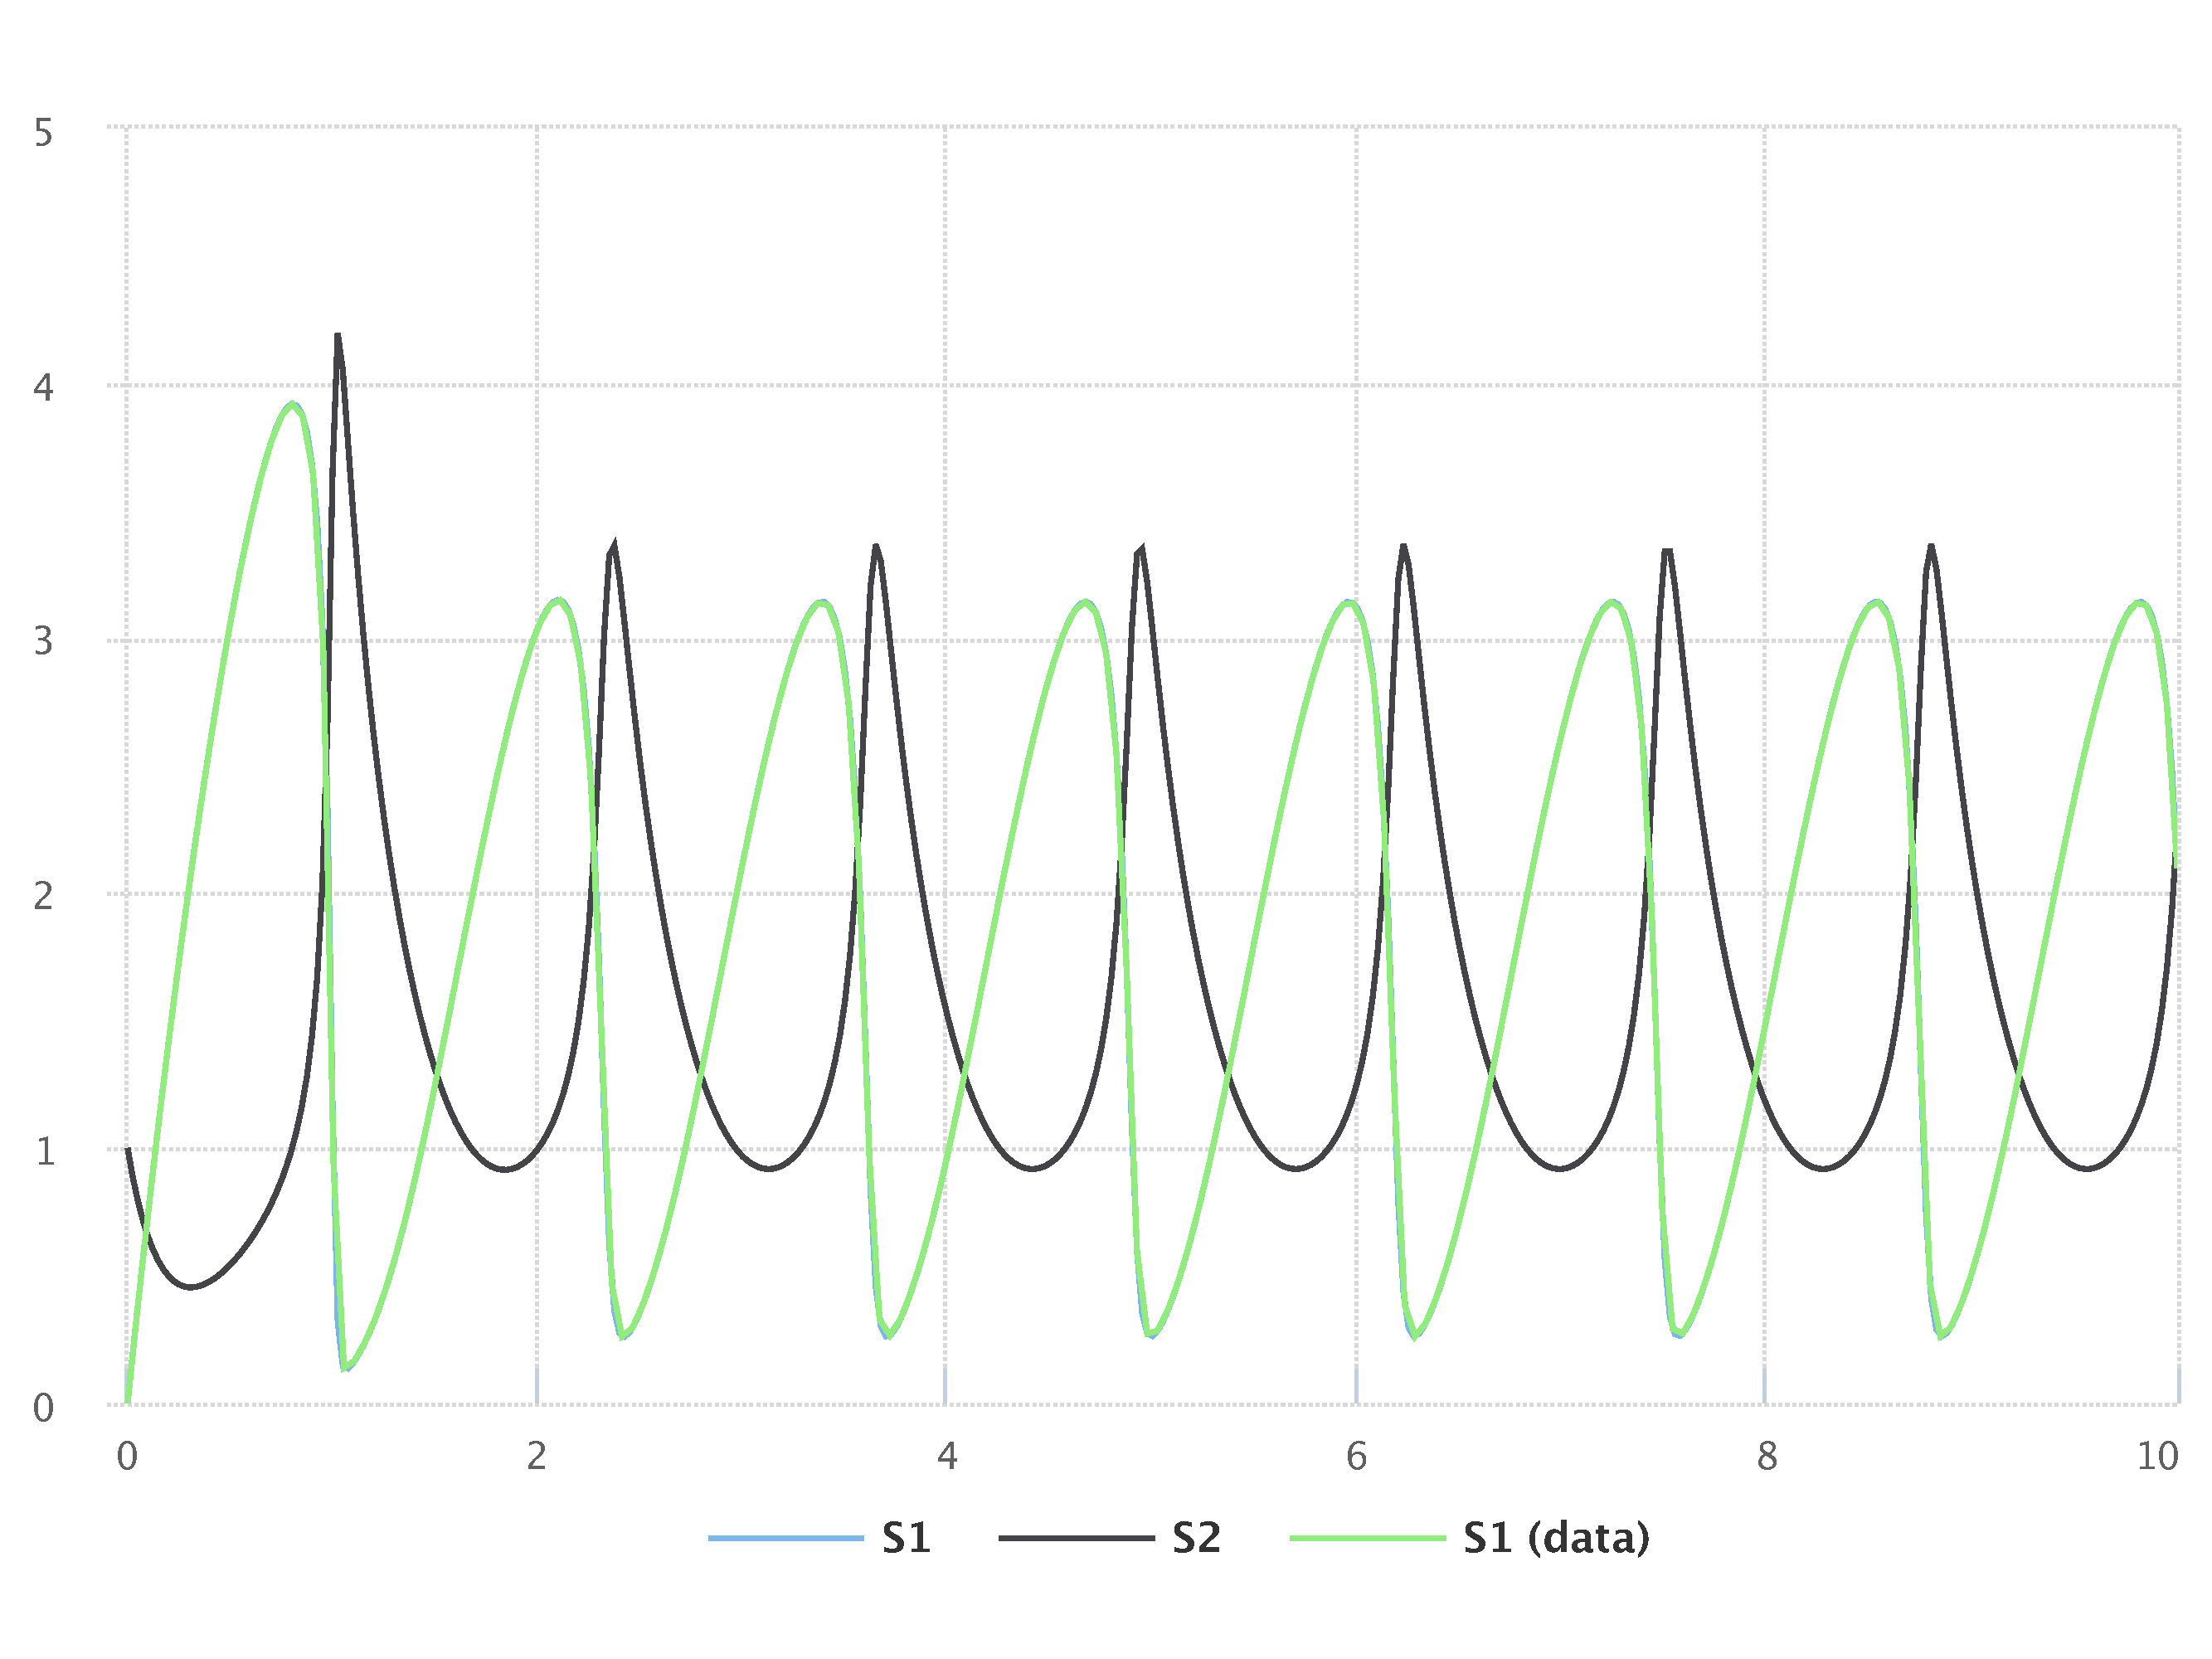
\includegraphics[width=1.0\textwidth]{examples/plotting-data-numl/results/sedml_webtools/plot1}
        \caption{The simulation result from the simulation description given in \lst{plotting-data-numl}. Simulation with SED-ML web tools \citep{bergmann2017sed}.}
    \end{minipage}\hfill
    \begin{minipage}{0.47\textwidth}
        \centering
        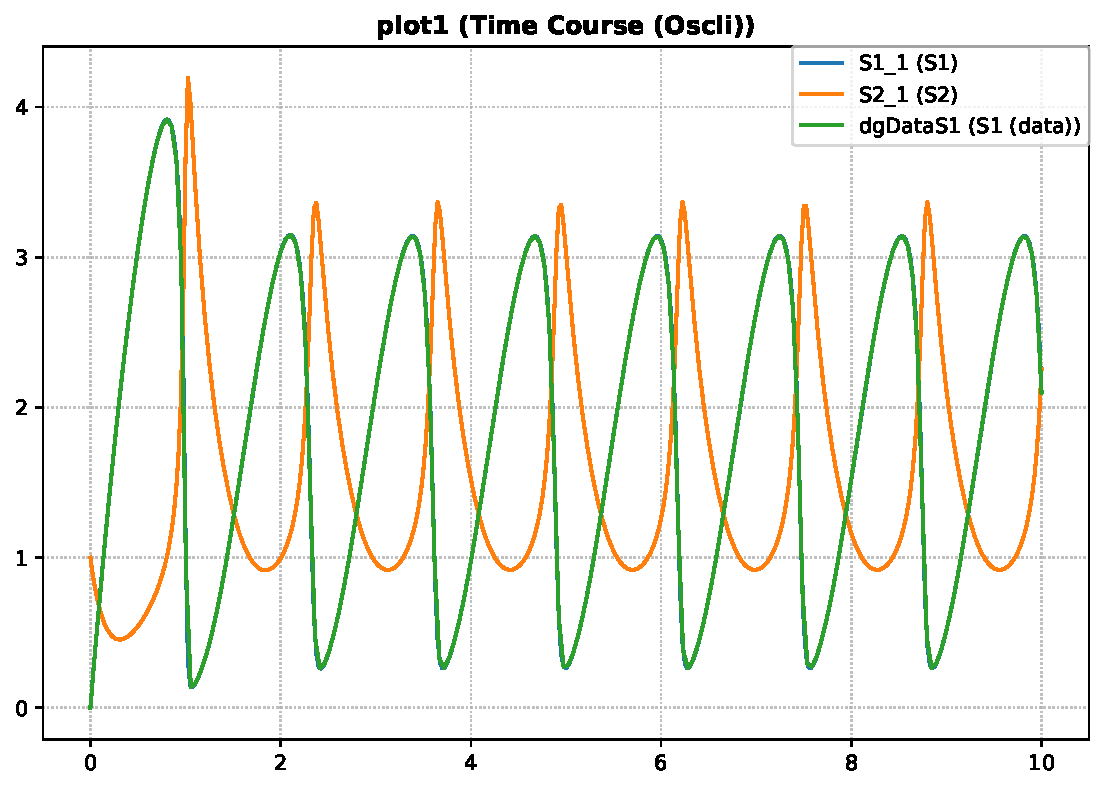
\includegraphics[width=1.0\textwidth]{examples/plotting-data-numl/results/tellurium/plot1}
        \caption{Simulation with tellurium \citep{tellurium}.}
    \end{minipage}
    \label{fig:plotting-data}
\end{figure}

\myXmlImport{SED-ML document using \SedDataSource and \SedDataDescription}
{lst:plotting-data-numl}
{examples/plotting-data-numl/plotting-data-numl.xml}

\pagebreak
% ~~~~~~~~~~~~~~~~~~~~~~~~~~~~~~~~~~~~
% REPEATED TASKS
% ~~~~~~~~~~~~~~~~~~~~~~~~~~~~~~~~~~~~
\section{Simulation experiments with repeatedTasks}
The \RepeatedTask makes it possible to encode a large number of different simulation experiments. In this section several such simulation experiments are presented.

% ~~~ TIME COURSE PARAMETER SCAN ~~~
\subsection{Time course parameter scan (\texttt{L1V3\_repeated-scan-oscli.omex})}
In this example a \hyperref[class:repeatedTask]{repeatedTask} is used to run repeated \hyperref[class:uniformTimeCourse]{uniformTimeCourse} simulations with a deterministic simulation algorithm. Within the \hyperref[class:repeatedTask]{repeatedTask} after each run the parameter value is changed, resulting in a time course parameter scan.

NOTE: This example produces three dimensional results (time, species concentration, multiple repeats).  SED-ML \currentLV \changed{provides ways to post-process these values with the \element{dimensionTerm} of the \Variable class, but here they are not used, meaning that every individual element in the \element{xDataReference} is plotted vs. every individual element in the \element{yDataReference}, effectively flattening the values by overlaying them onto the desired plot.  The breaks between dimensions should be used as breaks between any connected lines, so that spurious lines from the end of one plot to the beginning of the next are not present.  This document can be found at \url{https://sed-ml.org/examples/L1V3/L1V3_repeated-scan-oscli/repeated-scan-oscli.xml}, and an OMEX version at \url{https://sed-ml.org/examples/L1V3/L1V3_repeated-scan-oscli.omex}.}

\begin{figure}[ht]
    \centering
    \begin{minipage}{0.47\textwidth}
        \centering
        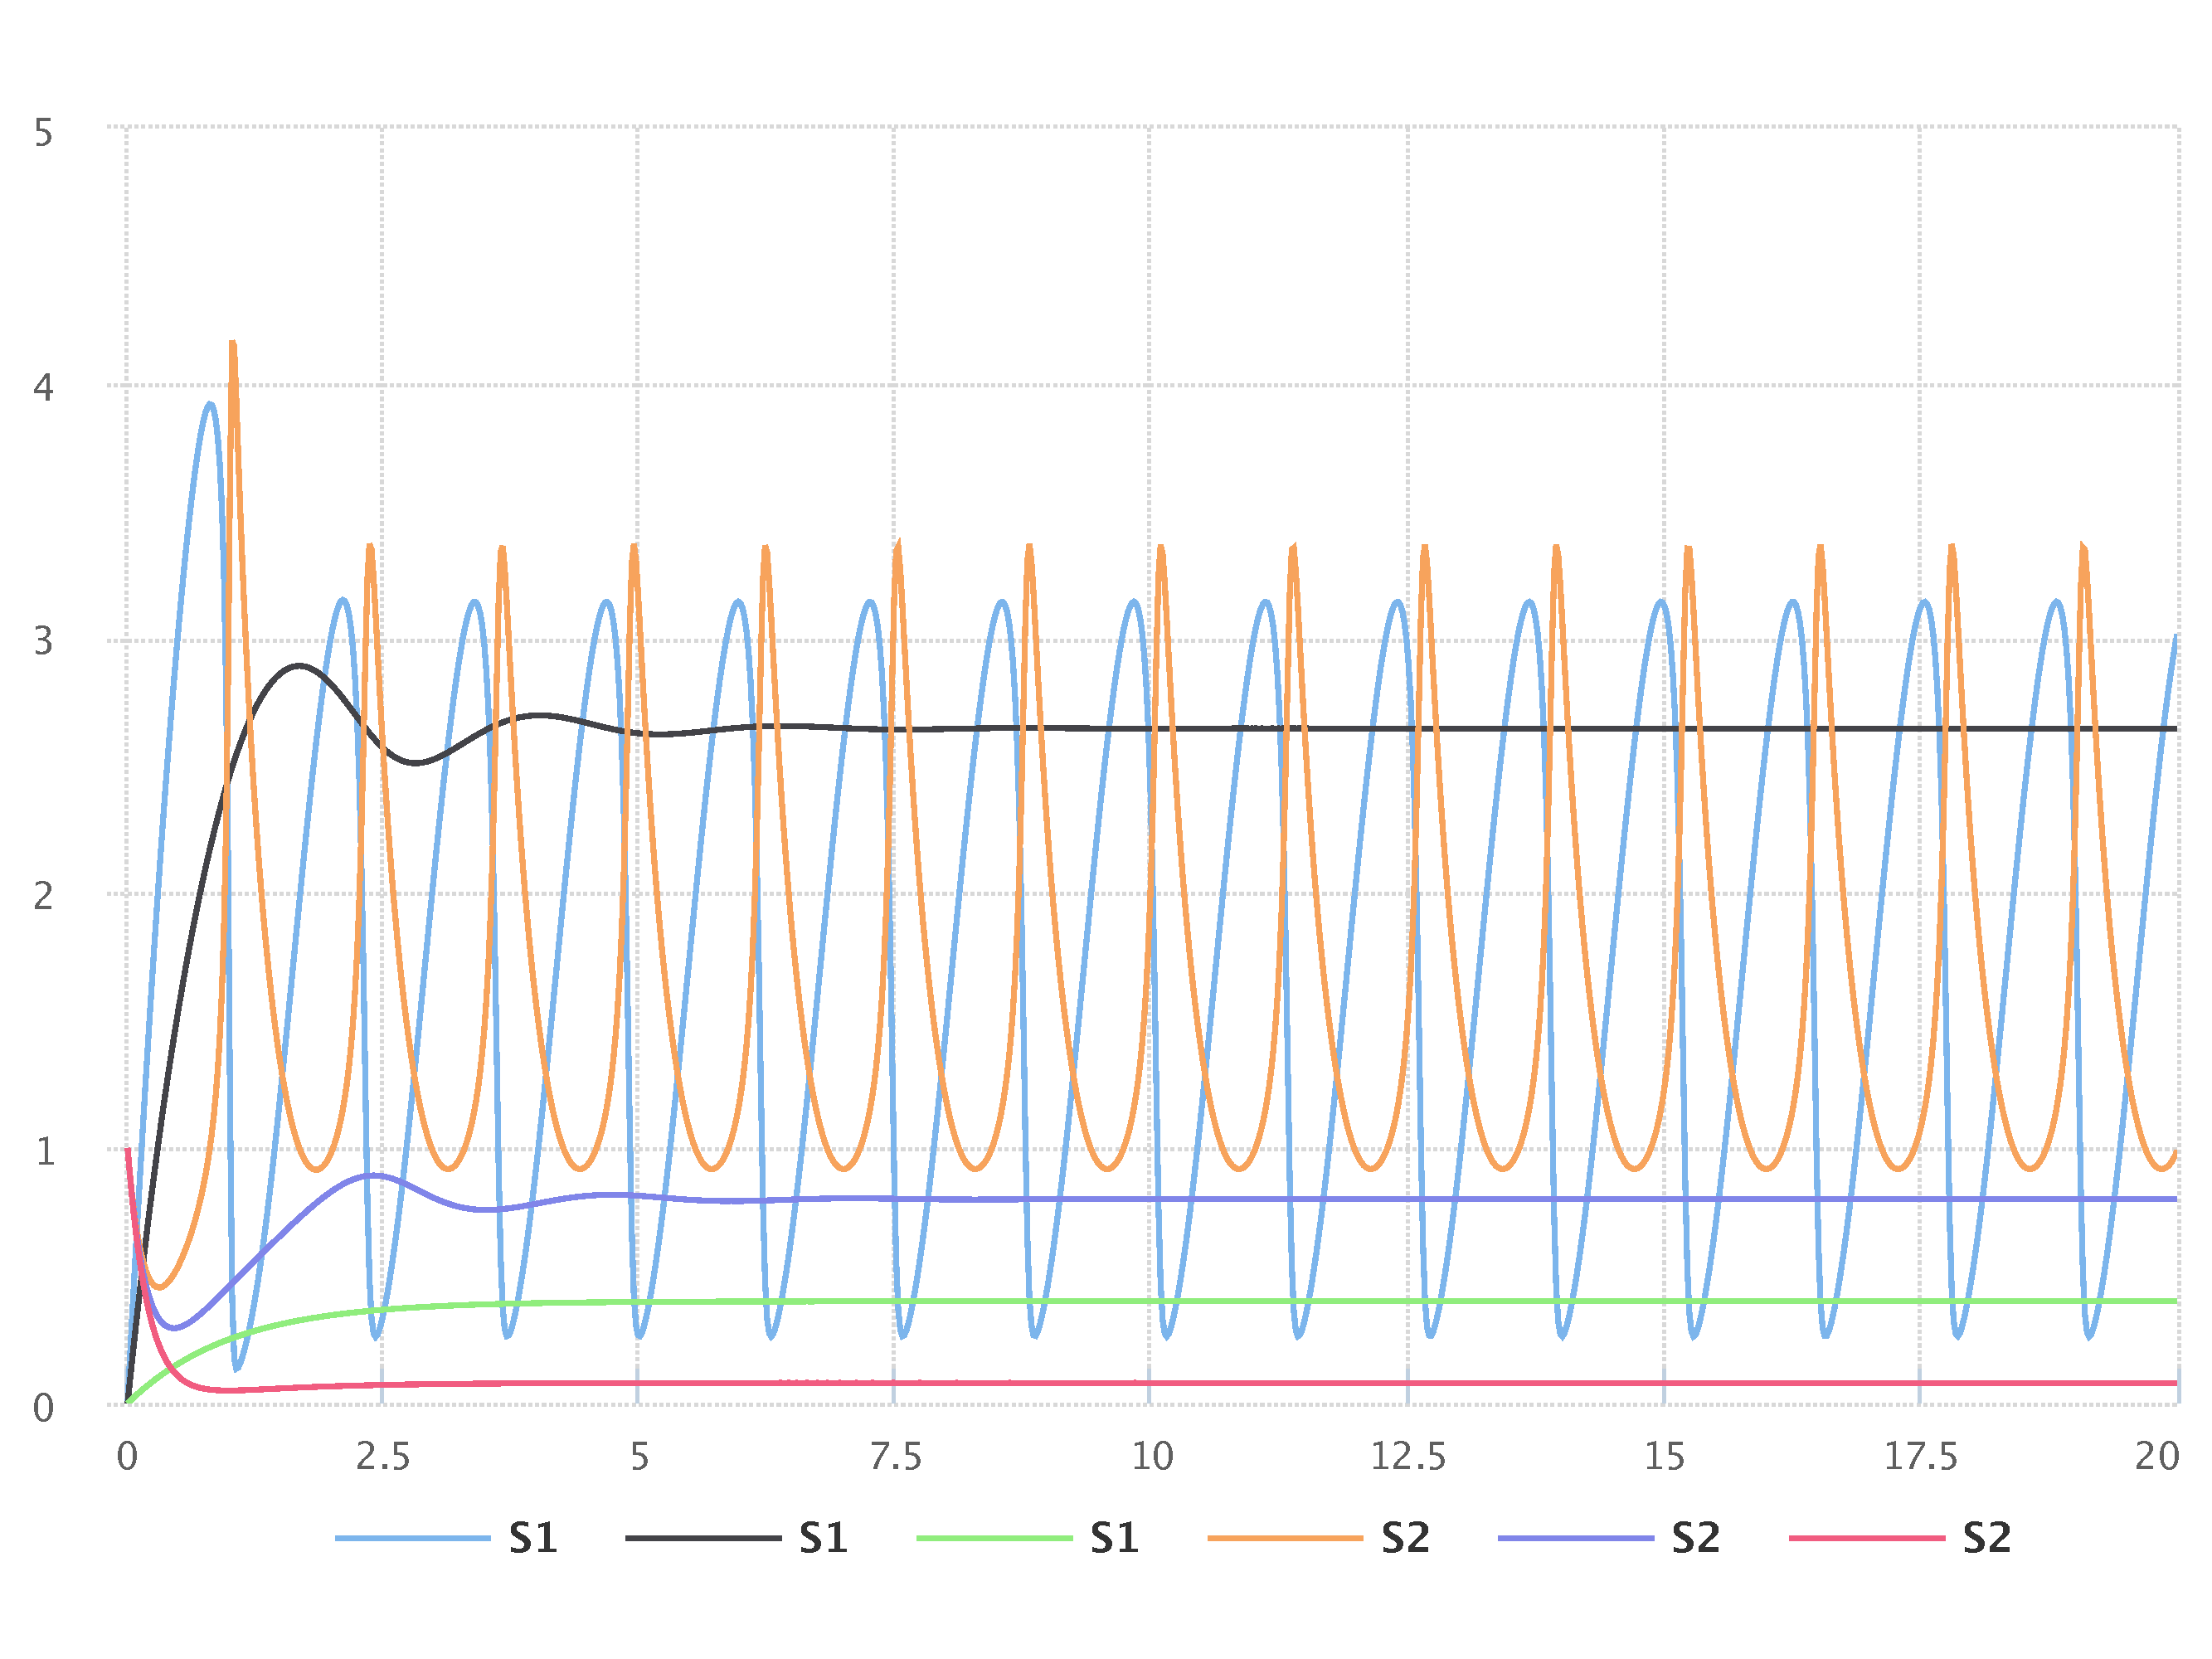
\includegraphics[width=1.0\textwidth]{examples/repeated-scan-oscli/results/sedml_webtools/plot1}
        \caption{The simulation result gained from the simulation description given in \lst{repeated-scan-oscli}. Simulation with SED-ML web tools \citep{bergmann2017sed}.}
    \end{minipage}\hfill
    \begin{minipage}{0.47\textwidth}
        \centering
                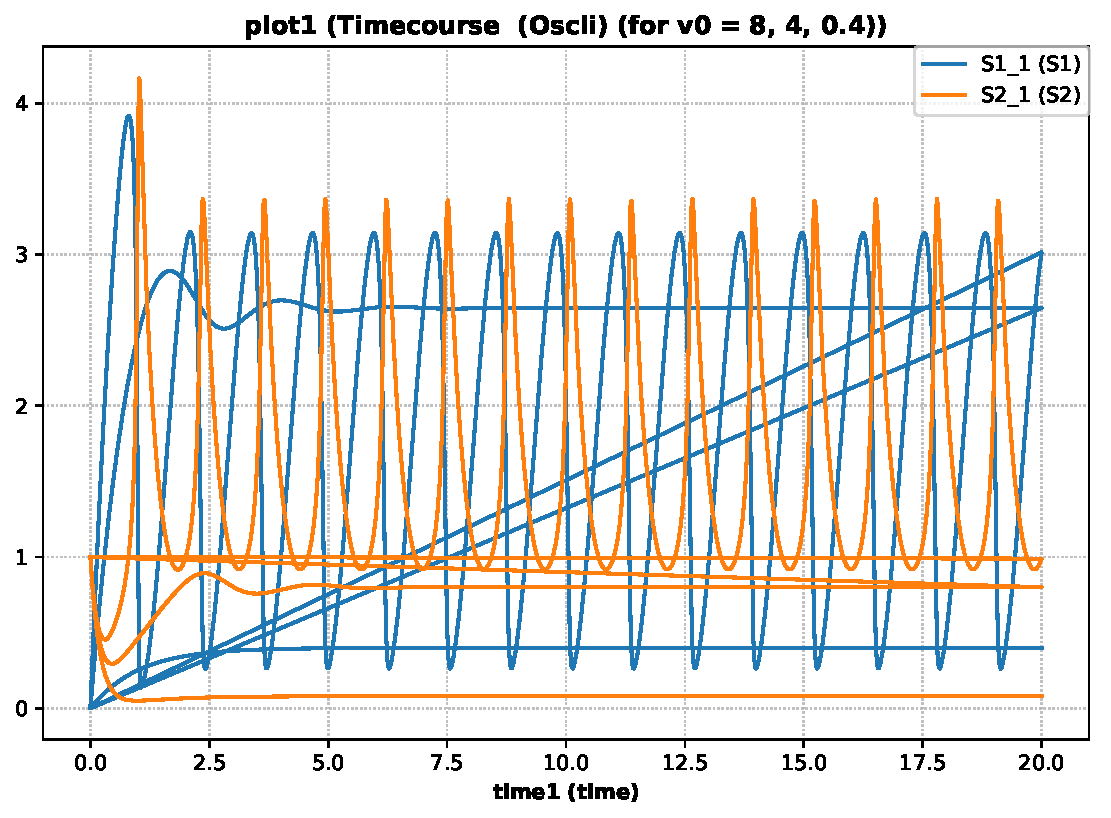
\includegraphics[width=1.0\textwidth]{examples/repeated-scan-oscli/results/tellurium/plot1}
        \caption{Simulation with tellurium \citep{tellurium}.}
    \end{minipage}
    \label{fig:repeated-scan-oscli}
\end{figure}

\myXmlImport{SED-ML document implementing the one dimensional time course parameter scan}
{lst:repeated-scan-oscli}
{examples/repeated-scan-oscli/repeated-scan-oscli.xml}

% ~~~ STEADY STATE PARAMETER SCAN ~~~
\subsection{Steady state parameter scan (\texttt{L1V3\_repeated-steady-scan-oscli.omex})}
In this example a \hyperref[class:repeatedTask]{repeatedTask} is used in combination with a \hyperref[class:steadyState]{steadyState} simulation task (performing a steady state computation). On each repeat a parameter is varied resulting in a steady state parameter scan.  \changed{This document can be found at \url{https://sed-ml.org/examples/L1V3/L1V3_repeated-steady-scan-oscli/repeated-steady-scan-oscli.xml}, and an OMEX version at \url{https://sed-ml.org/examples/L1V3/L1V3_repeated-steady-scan-oscli.omex}.}

\begin{figure}[ht!]
    \centering
    \begin{minipage}{0.47\textwidth}
        \centering
        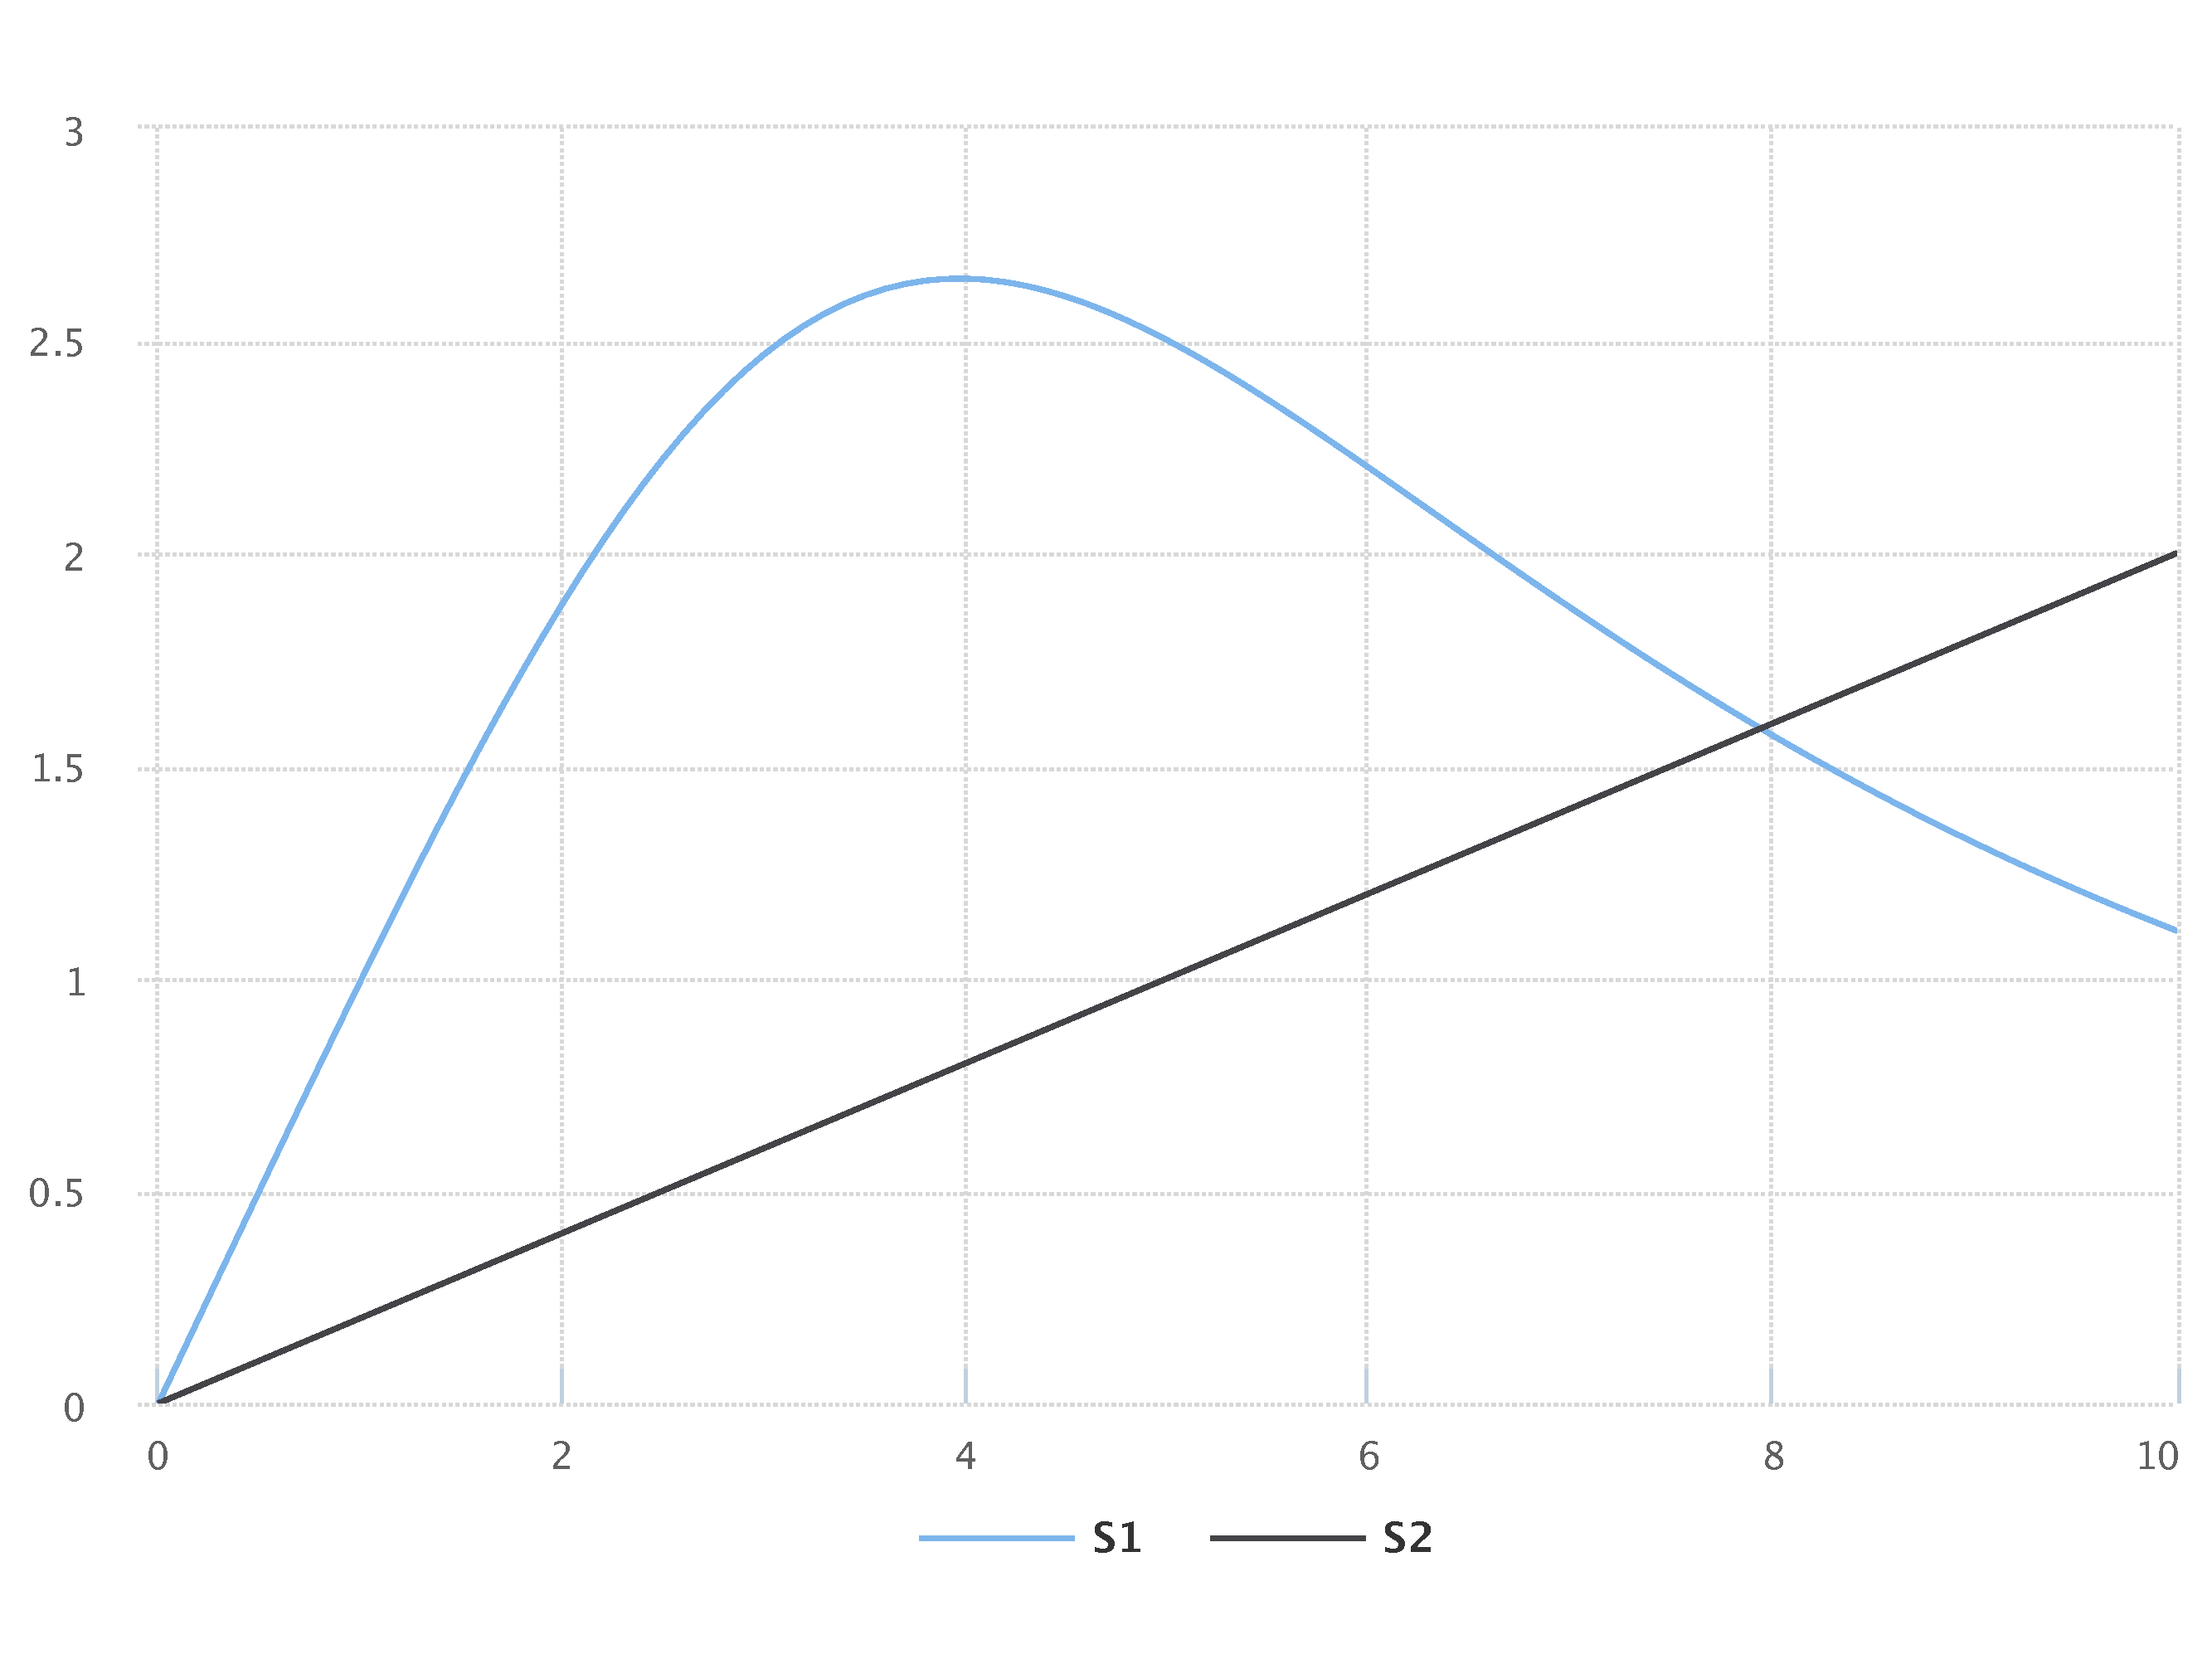
\includegraphics[width=1.0\textwidth]{examples/repeated-steady-scan-oscli/results/sedml_webtools/plot1}
        \caption{The simulation result from the simulation description given in \lst{repeated-steady-scan-oscli}. Simulation with SED-ML web tools \citep{bergmann2017sed}.}
    \end{minipage}\hfill
    \begin{minipage}{0.47\textwidth}
        \centering
        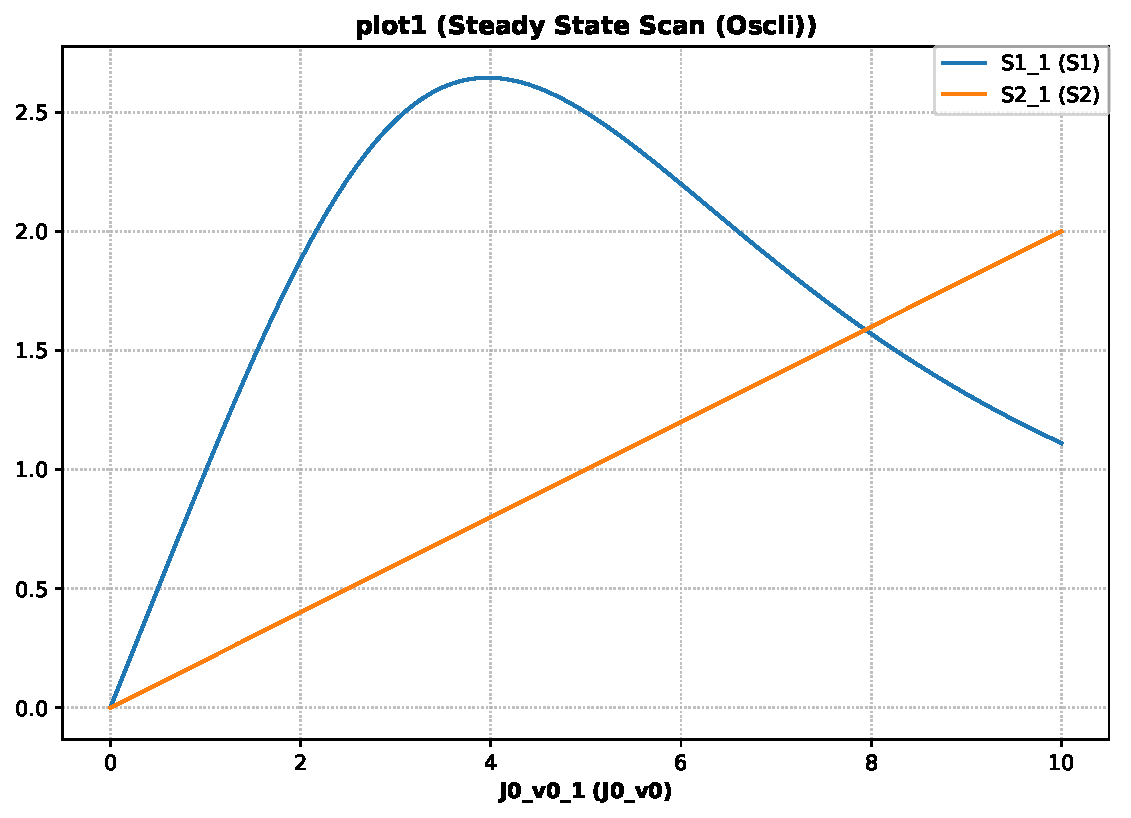
\includegraphics[width=1.0\textwidth]{examples/repeated-steady-scan-oscli/results/tellurium/plot1}
        \caption{Simulation with tellurium \citep{tellurium}.}
    \end{minipage}
    \label{fig:repeated-steady-scan-oscli}
\end{figure}

\myXmlImport{SED-ML document implementing the one dimensional steady state parameter scan}
{lst:repeated-steady-scan-oscli}
{examples/repeated-steady-scan-oscli/repeated-steady-scan-oscli.xml}


% ~~~ STOCHASTIC SIMULATION ~~~
\subsection{Stochastic simulation (\texttt{L1V3\_repeated-stochastic-runs.omex})}
In this example a \hyperref[class:repeatedTask]{repeatedTask} is used to run a stochastic simulation multiple times.
Running just one stochastic trace does not provide a complete picture of the behavior of a system. A large number of such traces is needed. This example demonstrates the basic use case of running ten traces of a simulation by using a \hyperref[class:repeatedTask]{repeatedTask} which runs ten uniform time course simulations (each performing a stochastic simulation run).

NOTE: This example produces three dimensional results (time, species concentration, multiple repeats). SED-ML \currentLV \changed{provides ways to post-process these values with the \element{dimensionTerm} of the \Variable class, but here they are not used, meaning that every individual element in the \element{xDataReference} is plotted vs. every individual element in the \element{yDataReference}, effectively flattening the values by overlaying them onto the desired plot.  The breaks between dimensions should be used as breaks between any connected lines, so that spurious lines from the end of one plot to the beginning of the next are not present.}

\changed{This document can be found at \url{https://sed-ml.org/examples/L1V3/L1V3_repeated-stochastic-runs/repeated-stochastic-runs.xml}, and an OMEX version at \url{https://sed-ml.org/examples/L1V3/L1V3_repeated-stochastic-runs.omex}.}

\begin{figure}[ht]
    \centering
    \begin{minipage}{0.47\textwidth}
        \centering
        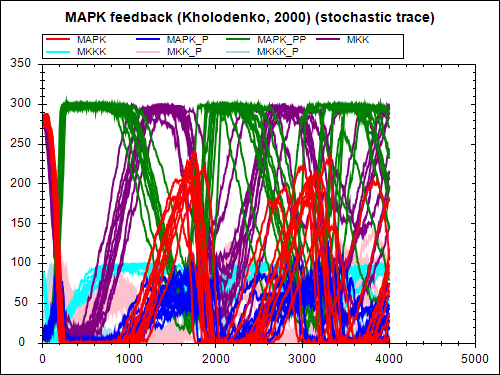
\includegraphics[width=1.0\textwidth]{examples/repeated-stochastic-runs/results/sedml_webtools/plot1}
        \caption{The simulation result from the simulation description given in \lst{repeated-stochastic-runs}. Simulation with SED-ML web tools \citep{bergmann2017sed}.}
    \end{minipage}\hfill
    \begin{minipage}{0.47\textwidth}
        \centering
        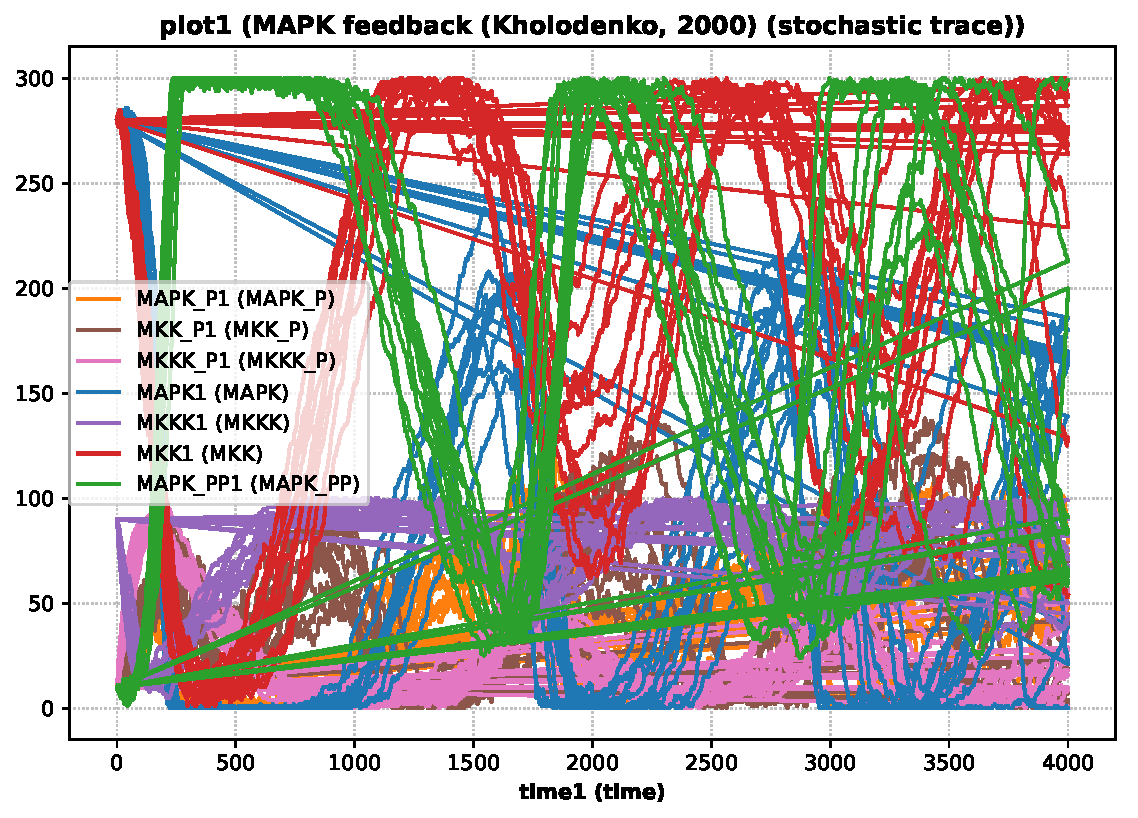
\includegraphics[width=1.0\textwidth]{examples/repeated-stochastic-runs/results/tellurium/plot1}
        \caption{Simulation with tellurium \citep{tellurium}.}
    \end{minipage}
    \label{fig:repeated-stochastic-runs}
\end{figure}

\myXmlImport{SED-ML document implementing repeated stochastic runs}
{lst:repeated-stochastic-runs}
{examples/repeated-stochastic-runs/repeated-stochastic-runs.xml}


% ~~~ SIMULATION PERTURBATION ~~~
\subsection{Simulation perturbation (\texttt{L1V3\_oscli-nested-pulse.omex})}
Often it is interesting to see how the dynamic behavior of a model changes when some perturbations are applied to the model. In this example a \hyperref[class:repeatedTask]{repeatedTask} is used iterating a \hyperref[class:oneStep]{oneStep} task (that advances an ODE integration to the next output step). During the steps a single parameter is modified effectively causing the oscillations of a model to stop. Once the value is reset the oscillations recover. 

Note: In the example a \hyperref[class:functionalRange]{functionalRange} is used, although the same result could also be achieved using the \hyperref[class:setValue]{setValue} element directly.

\changed{This document can be found at the URL \url{https://sed-ml.org/examples/L1V3/L1V3_oscli-nested-pulse/oscli-nested-pulse.xml}, and an OMEX version at the URL \url{https://sed-ml.org/examples/L1V3/L1V3_oscli-nested-pulse.omex}.}

\begin{figure}[ht]
    \centering
    \begin{minipage}{0.47\textwidth}
        \centering
        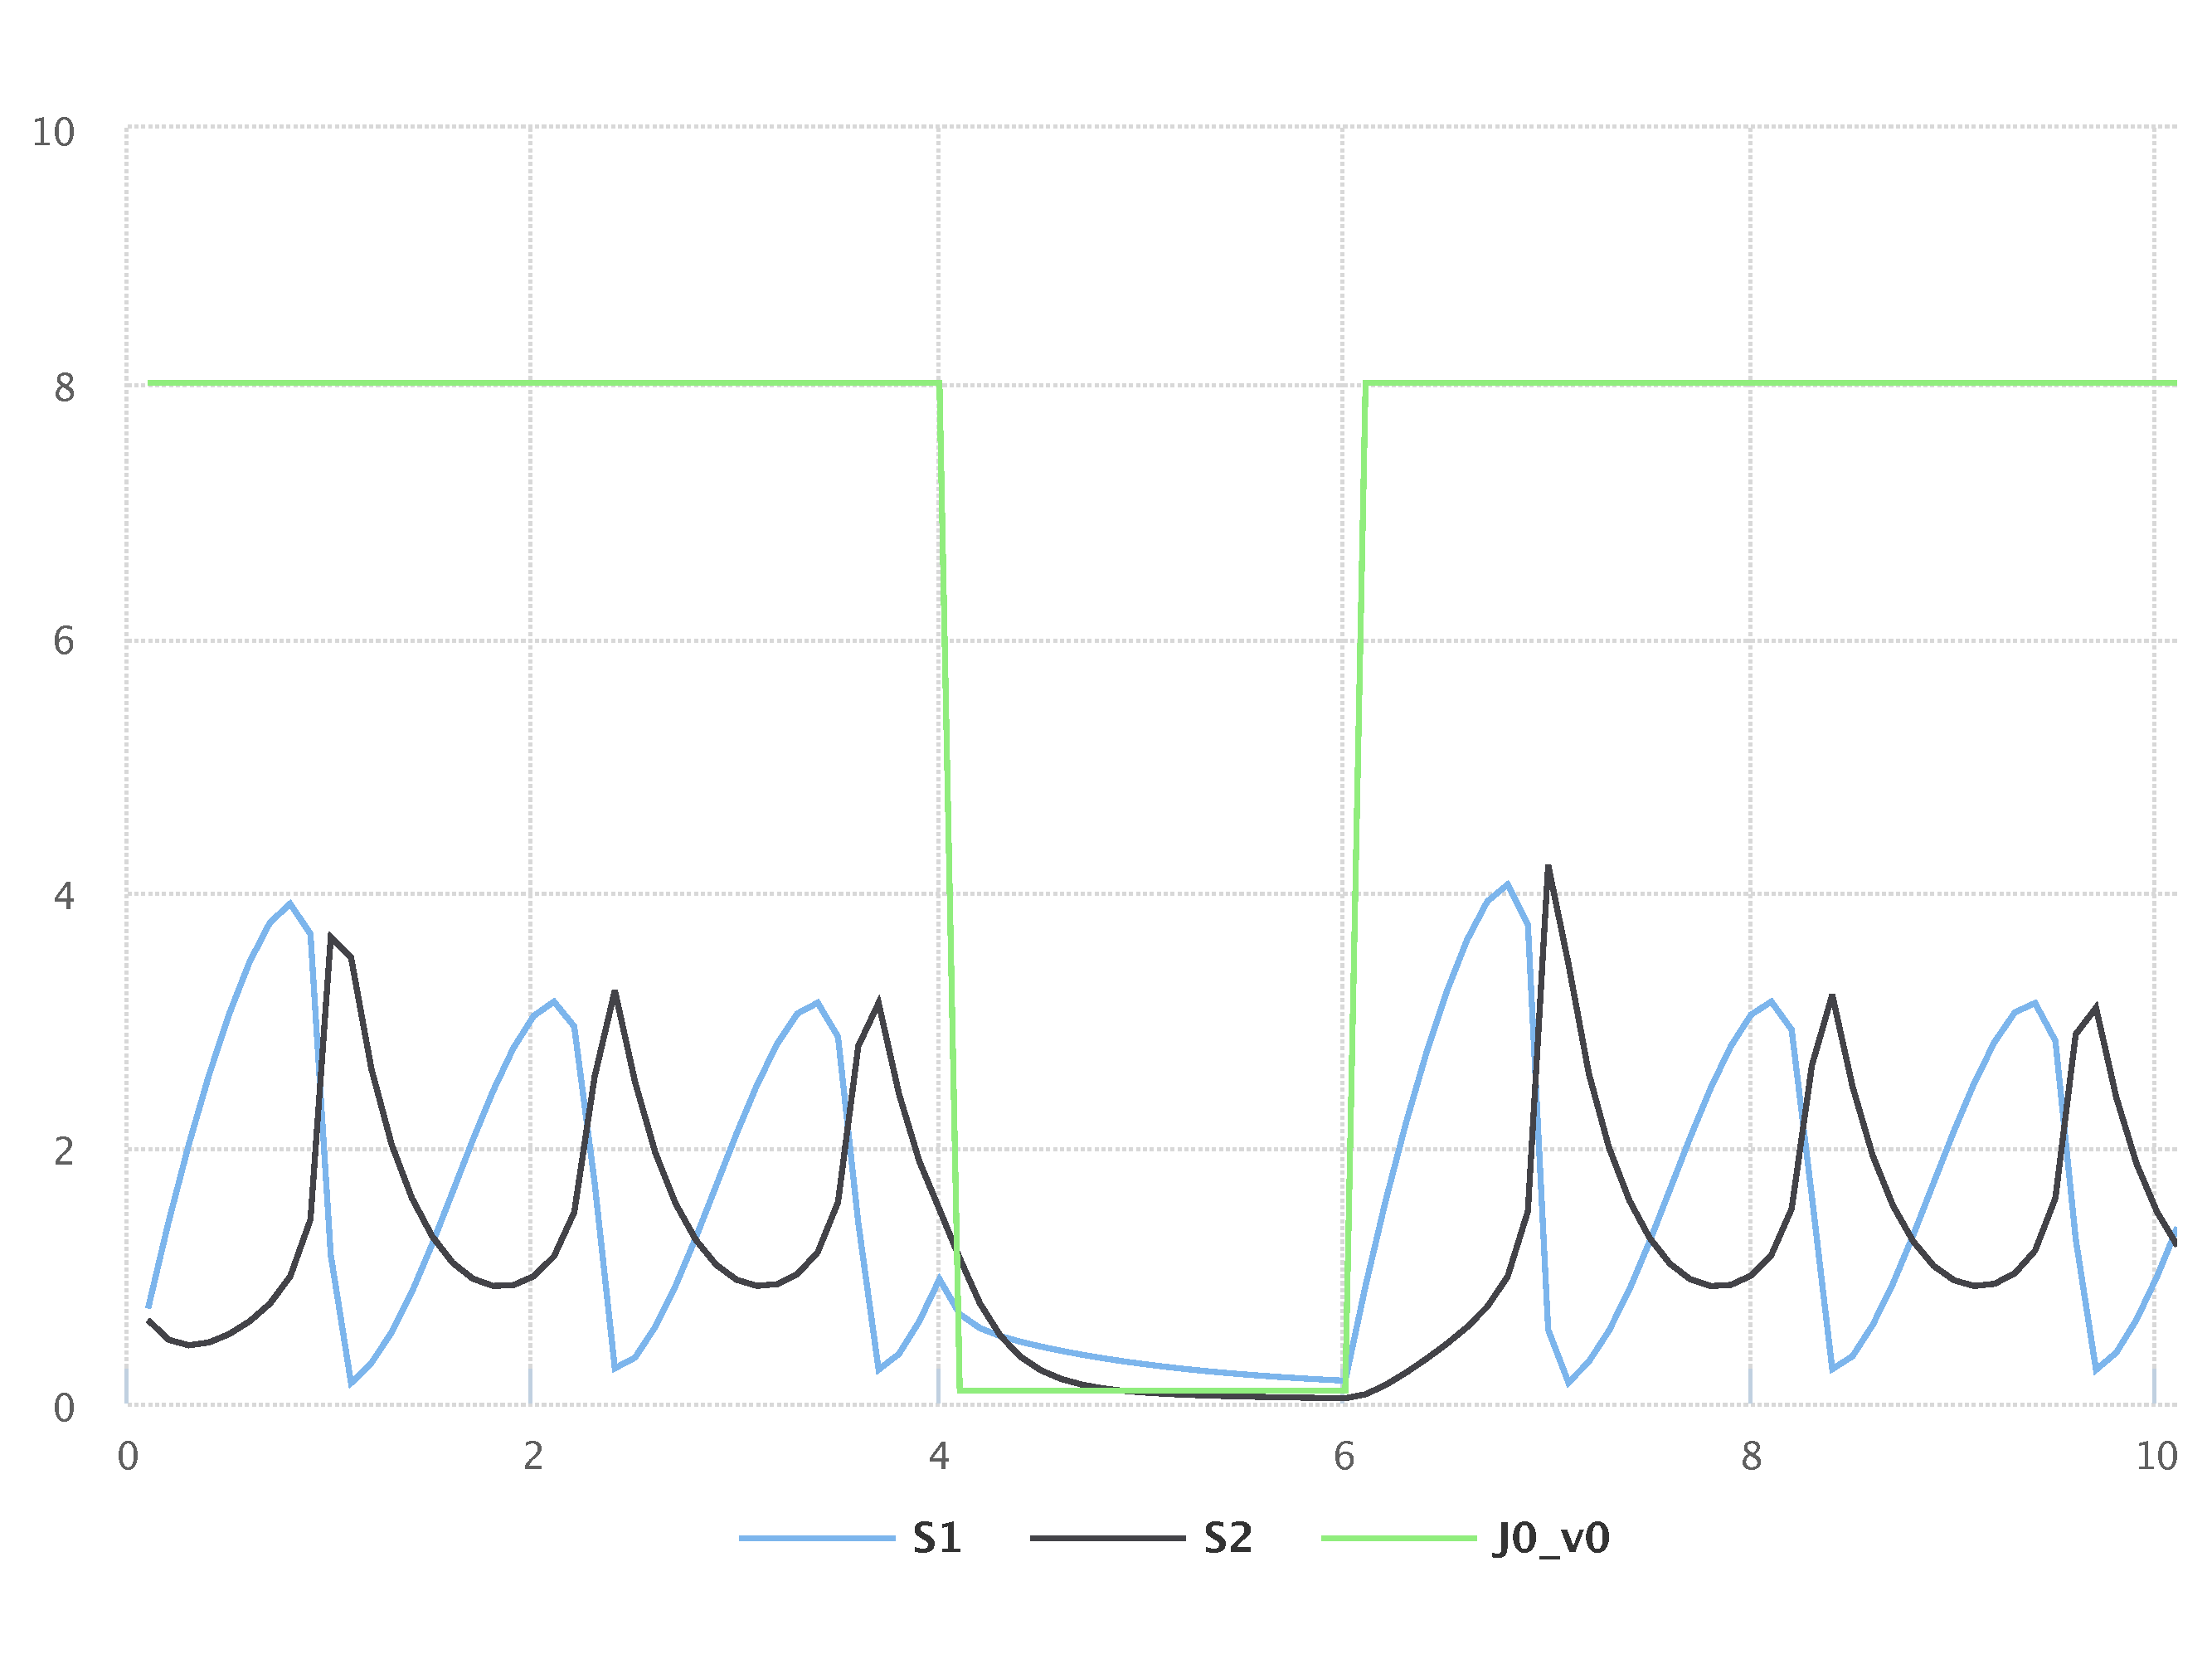
\includegraphics[width=1.0\textwidth]{examples/oscli-nested-pulse/results/sedml_webtools/plot1}
        \caption{The simulation result from the simulation description given in \lst{oscli-nested-pulse}. Simulation with SED-ML web tools \citep{bergmann2017sed}.}
    \end{minipage}\hfill
    \begin{minipage}{0.47\textwidth}
        \centering
        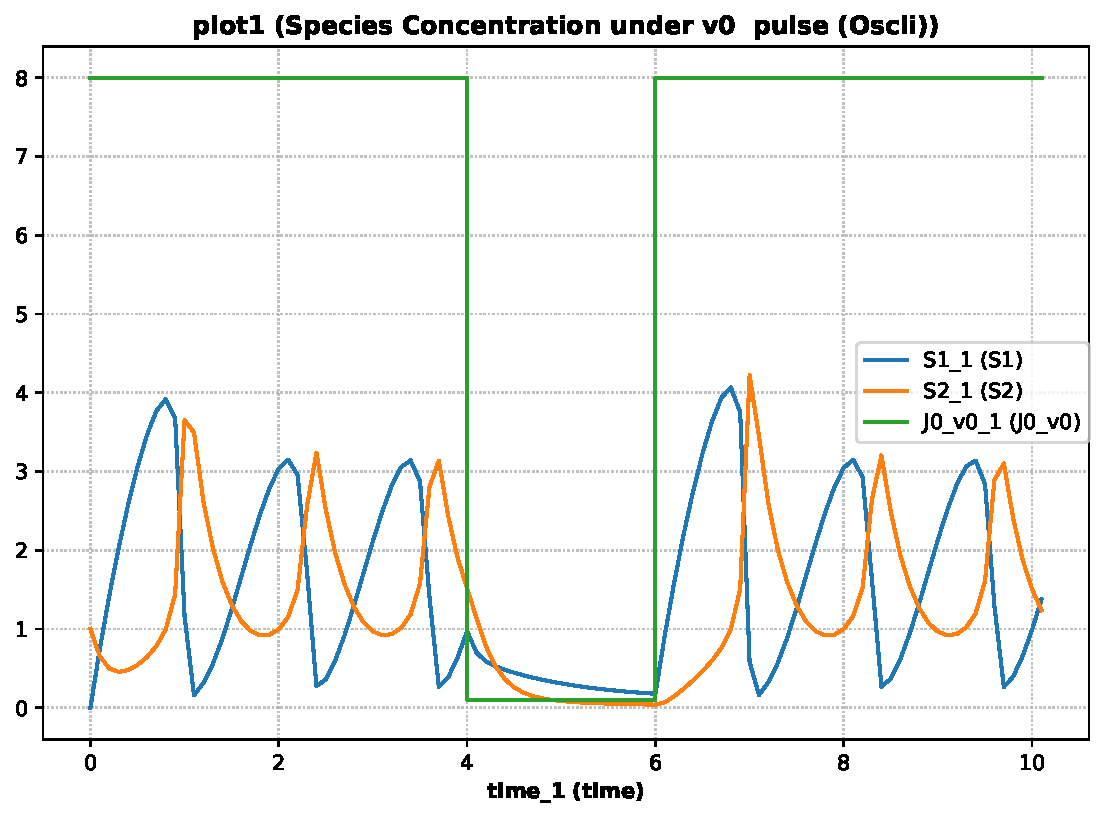
\includegraphics[width=1.0\textwidth]{examples/oscli-nested-pulse/results/tellurium/plot1}
        \caption{Simulation with tellurium \citep{tellurium}.}
    \end{minipage}
    \label{fig:oscli-nested-pulse}
\end{figure}

\myXmlImport{SED-ML document implementing the perturbation experiment}
{lst:oscli-nested-pulse}
{examples/oscli-nested-pulse/oscli-nested-pulse.xml}


% ~~~ 2D STEADY STATE PARAMETER SCAN ~~~
\subsection{2D steady state parameter scan (\texttt{L1V3\_parameter-scan-2d.omex})}
This example uses a \hyperref[class:repeatedTask]{repeatedTask} which runs over another \hyperref[class:repeatedTask]{repeatedTask} which performs a steady state computation. Each repeated simulation task modifies a different parameter.

NOTE: This example produces three dimensional results (time, species concentration, multiple repeats). SED-ML \currentLV \changed{provides ways to post-process these values with the \element{dimensionTerm} attribute of the \Variable class, but here they are not used, meaning that every individual element in the \element{xDataReference} is plotted vs. every individual element in the \element{yDataReference}, effectively flattening the values by overlaying them onto the desired plot.  The breaks between dimensions should be used as breaks between any connected lines, so that spurious lines from the end of one plot to the beginning of the next are not present.}

\changed{This document can be found at the URL \url{https://sed-ml.org/examples/L1V3/L1V3_parameter-scan-2d/parameter-scan-2d.xml}, and an OMEX version at the URL \url{https://sed-ml.org/examples/L1V3/L1V3_parameter-scan-2d.omex}.}

\begin{figure}[ht]
    \centering
    \begin{minipage}{0.47\textwidth}
        \centering
        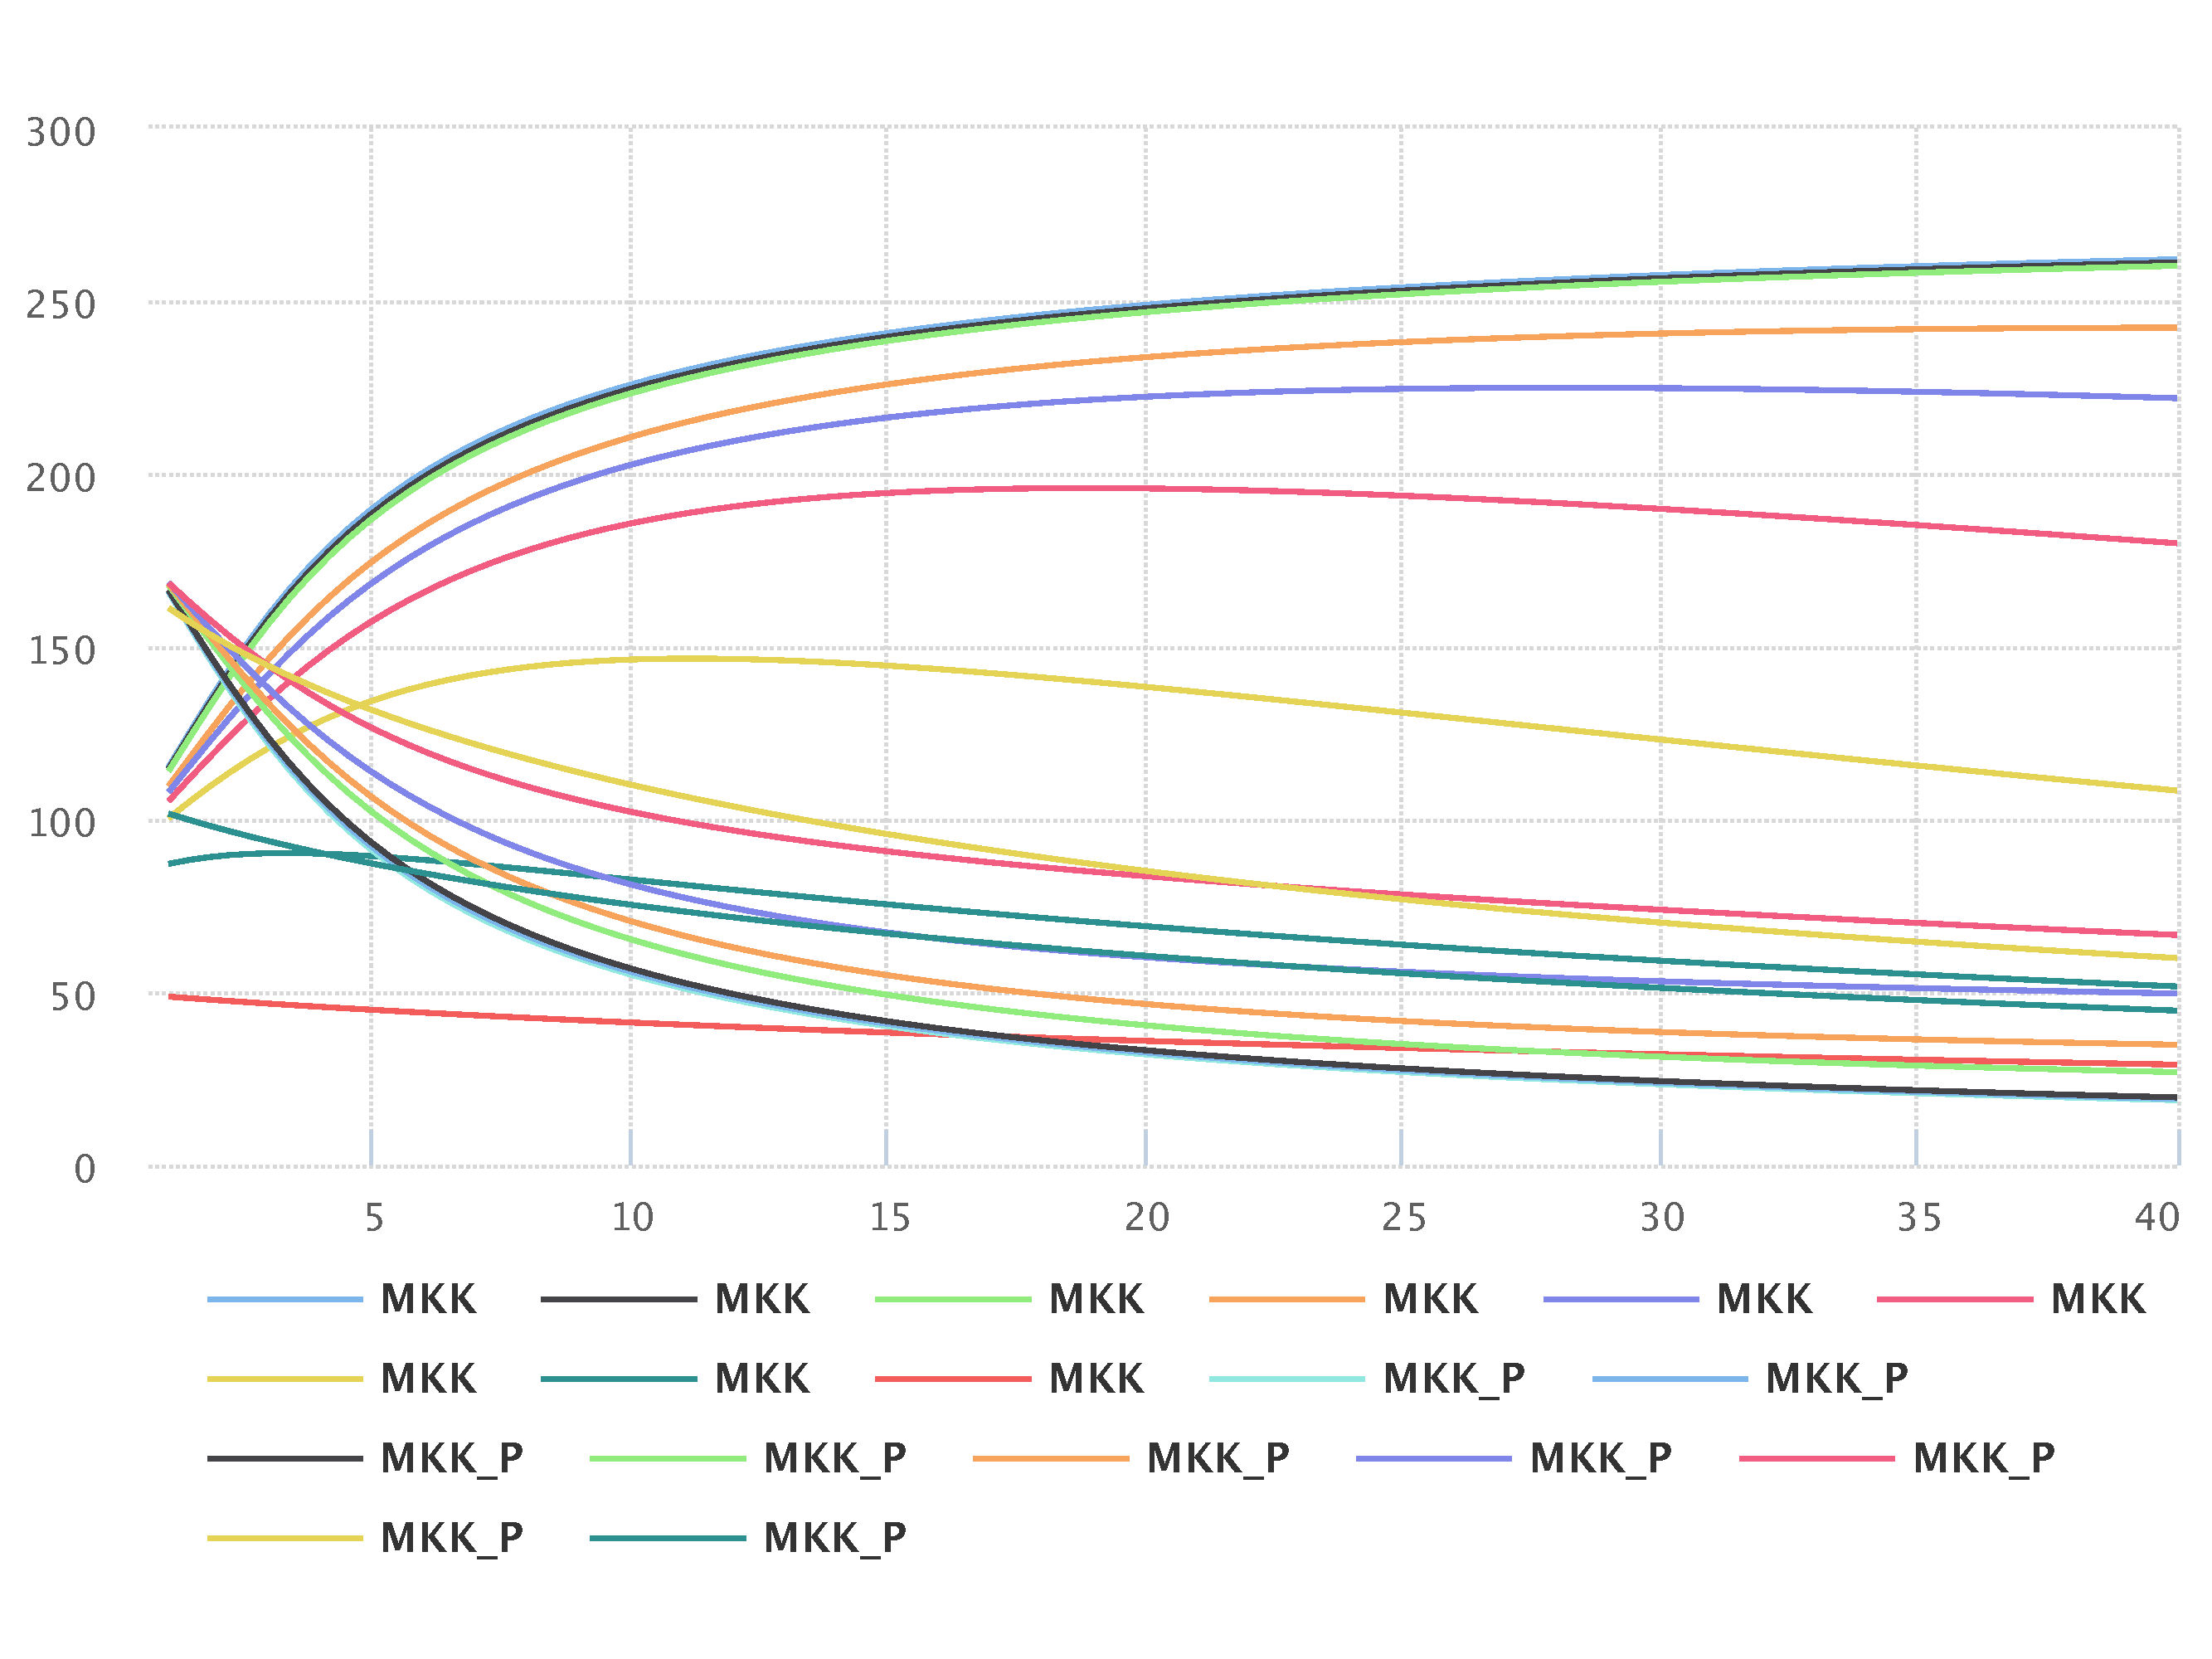
\includegraphics[width=1.0\textwidth]{examples/parameter-scan-2d/results/sedml_webtools/plot1}
        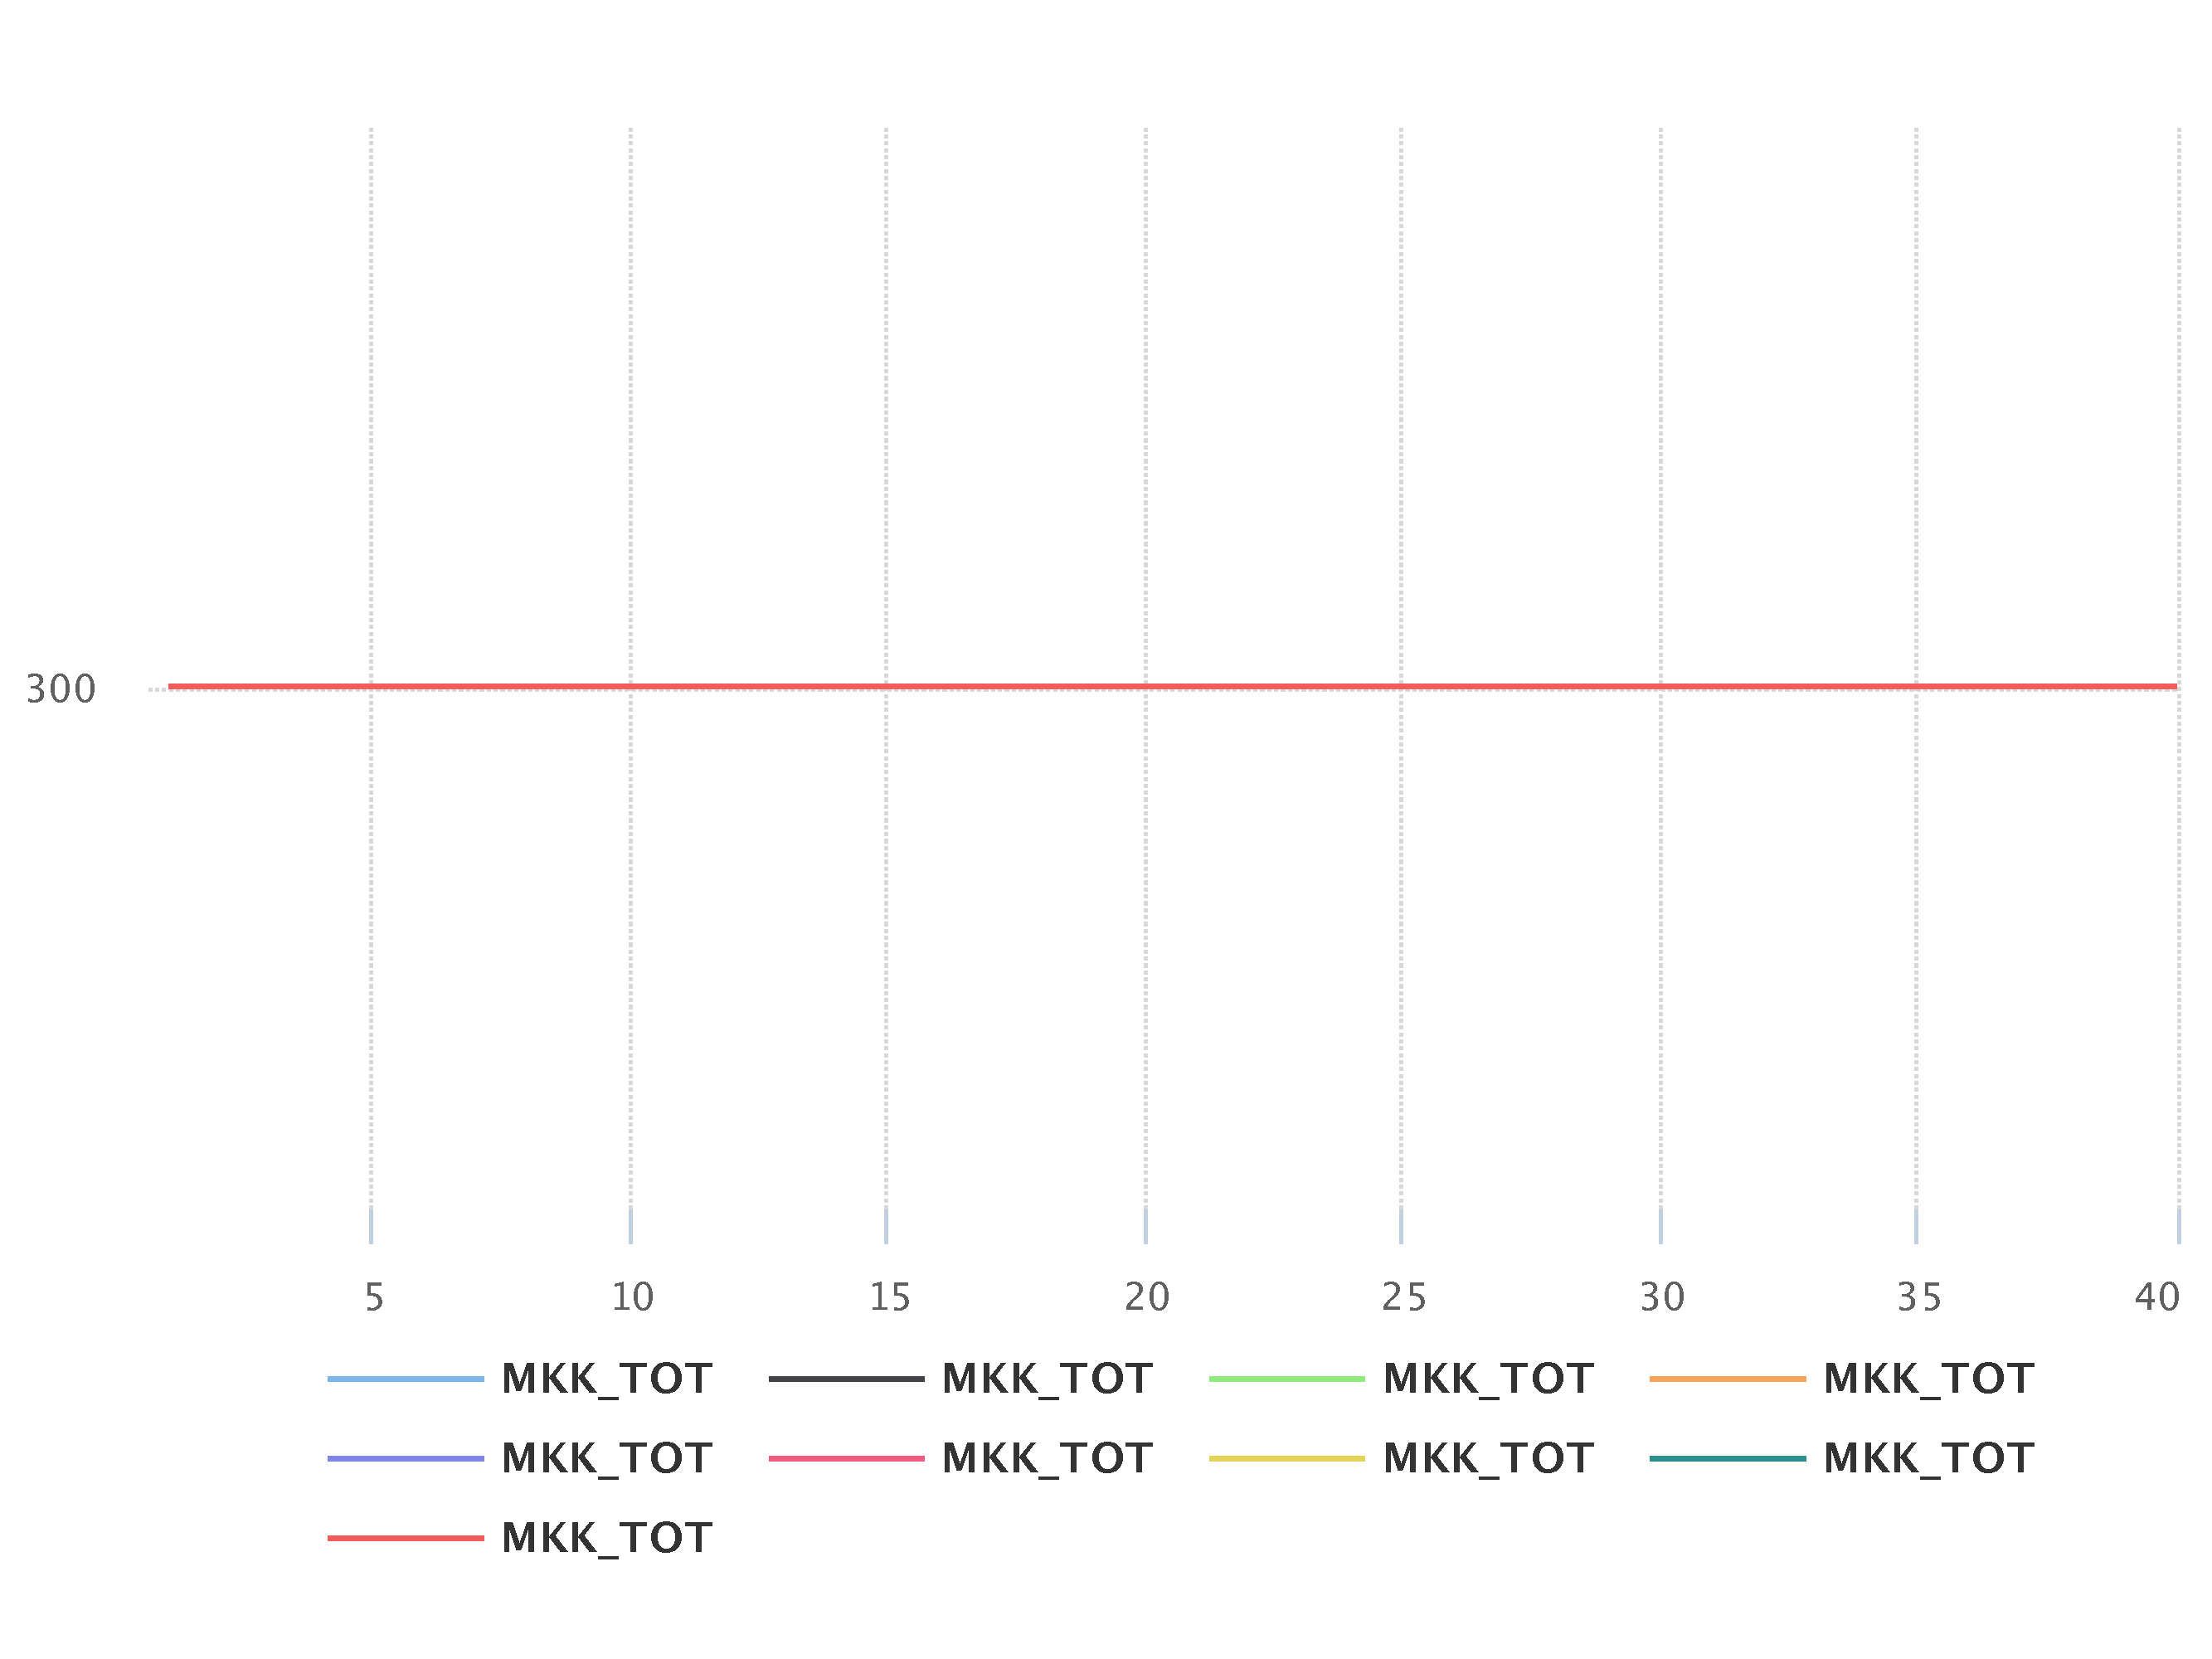
\includegraphics[width=1.0\textwidth]{examples/parameter-scan-2d/results/sedml_webtools/plot2}
        \caption{The simulation result gained from the simulation description given in \lst{parameter-scan-2d}. Simulation with SED-ML web tools \citep{bergmann2017sed}.}
    \end{minipage}\hfill
    \begin{minipage}{0.47\textwidth}
        \centering
        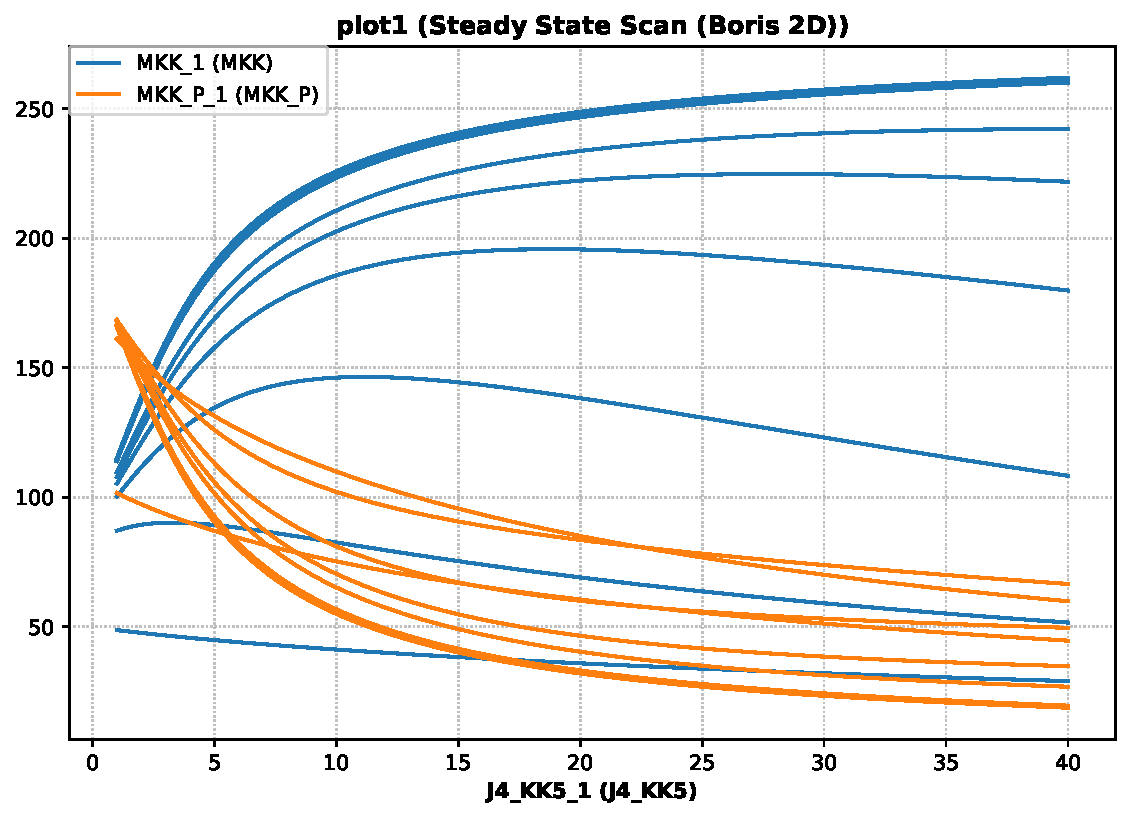
\includegraphics[width=1.0\textwidth]{examples/parameter-scan-2d/results/tellurium/plot1}
		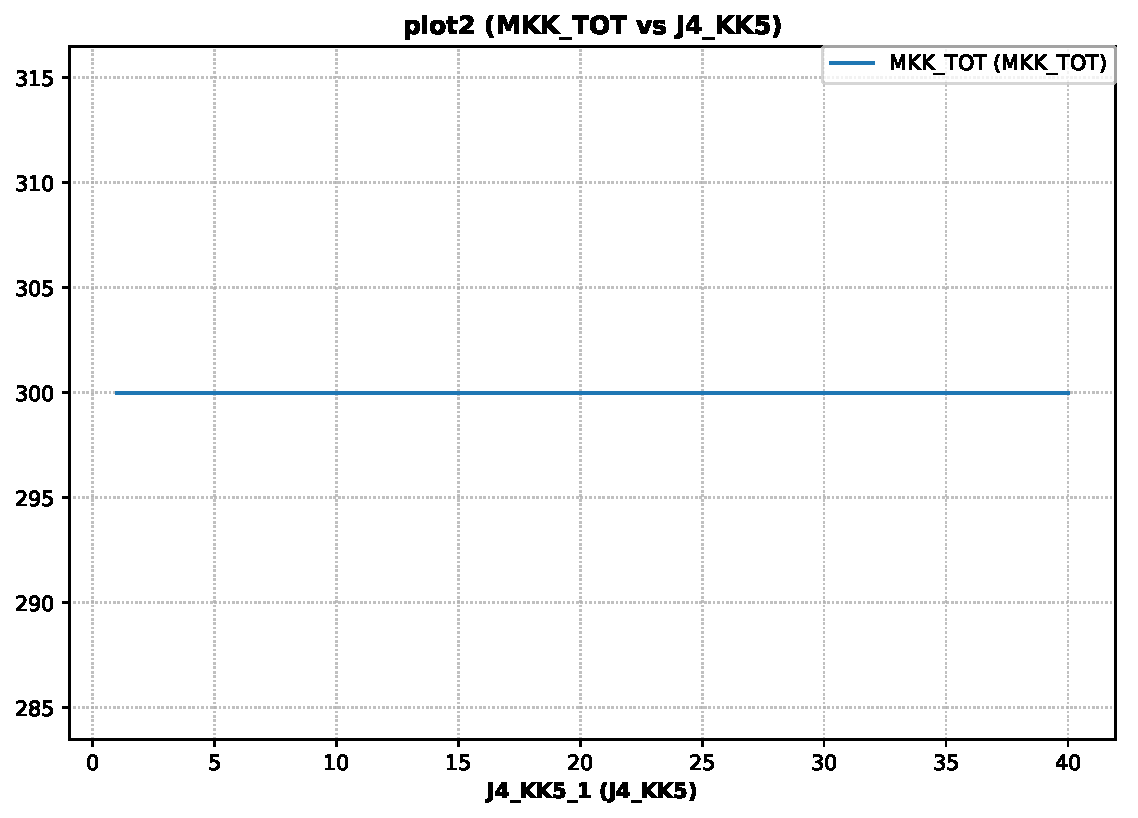
\includegraphics[width=1.0\textwidth]{examples/parameter-scan-2d/results/tellurium/plot2}
        \caption{Simulation with tellurium \citep{tellurium}.}
    \end{minipage}
    \label{fig:parameter-scan-2d}
\end{figure}

\myXmlImport{SED-ML document implementing the two dimensional steady state parameter scan}
{lst:parameter-scan-2d}
{examples/parameter-scan-2d/parameter-scan-2d.xml}

\pagebreak
% ~~~~~~~~~~~~~~~~~~~~~~~~~~~~~~~~~~~~
% DIFFERENT MODEL LANGUAGES
% ~~~~~~~~~~~~~~~~~~~~~~~~~~~~~~~~~~~~
\section{Simulation experiments with different model languages}
SED-ML allows to specify models in various languages, e.g., SBML \citep{Hucka:2003} and CellML \citep{cuellar:2003} (see Section~\ref{sec:languageURN} for more information). This section demonstrates the same simulation experiment with the model either in SBML (Appendix~\ref{example:vanderpol_sbml}) or in CellML (Appendix~\ref{example:vanderpol_cellml}).

\subsection{Van der Pol oscillator in SBML (\texttt{L1V3\_vanderpol-sbml.omex})}
\label{example:vanderpol_sbml}
The following example provides a SED-ML description for the simulation of the Van der Pol oscillator in SBML \citep{Hucka:2003}. The time-course and the behavior in the phase plane are plotted. The mathematical model and the performed simulation experiment are identical to Appendix~\ref{example:vanderpol_cellml}.  \changed{This document can be found at \url{https://sed-ml.org/examples/L1V3/L1V3_vanderpol-sbml/vanderpol.xml}, and an OMEX version at \url{https://sed-ml.org/examples/L1V3/L1V3_vanderpol-sbml.omex}.}

\begin{figure}[ht]
    \centering
    \begin{minipage}{0.47\textwidth}
        \centering
        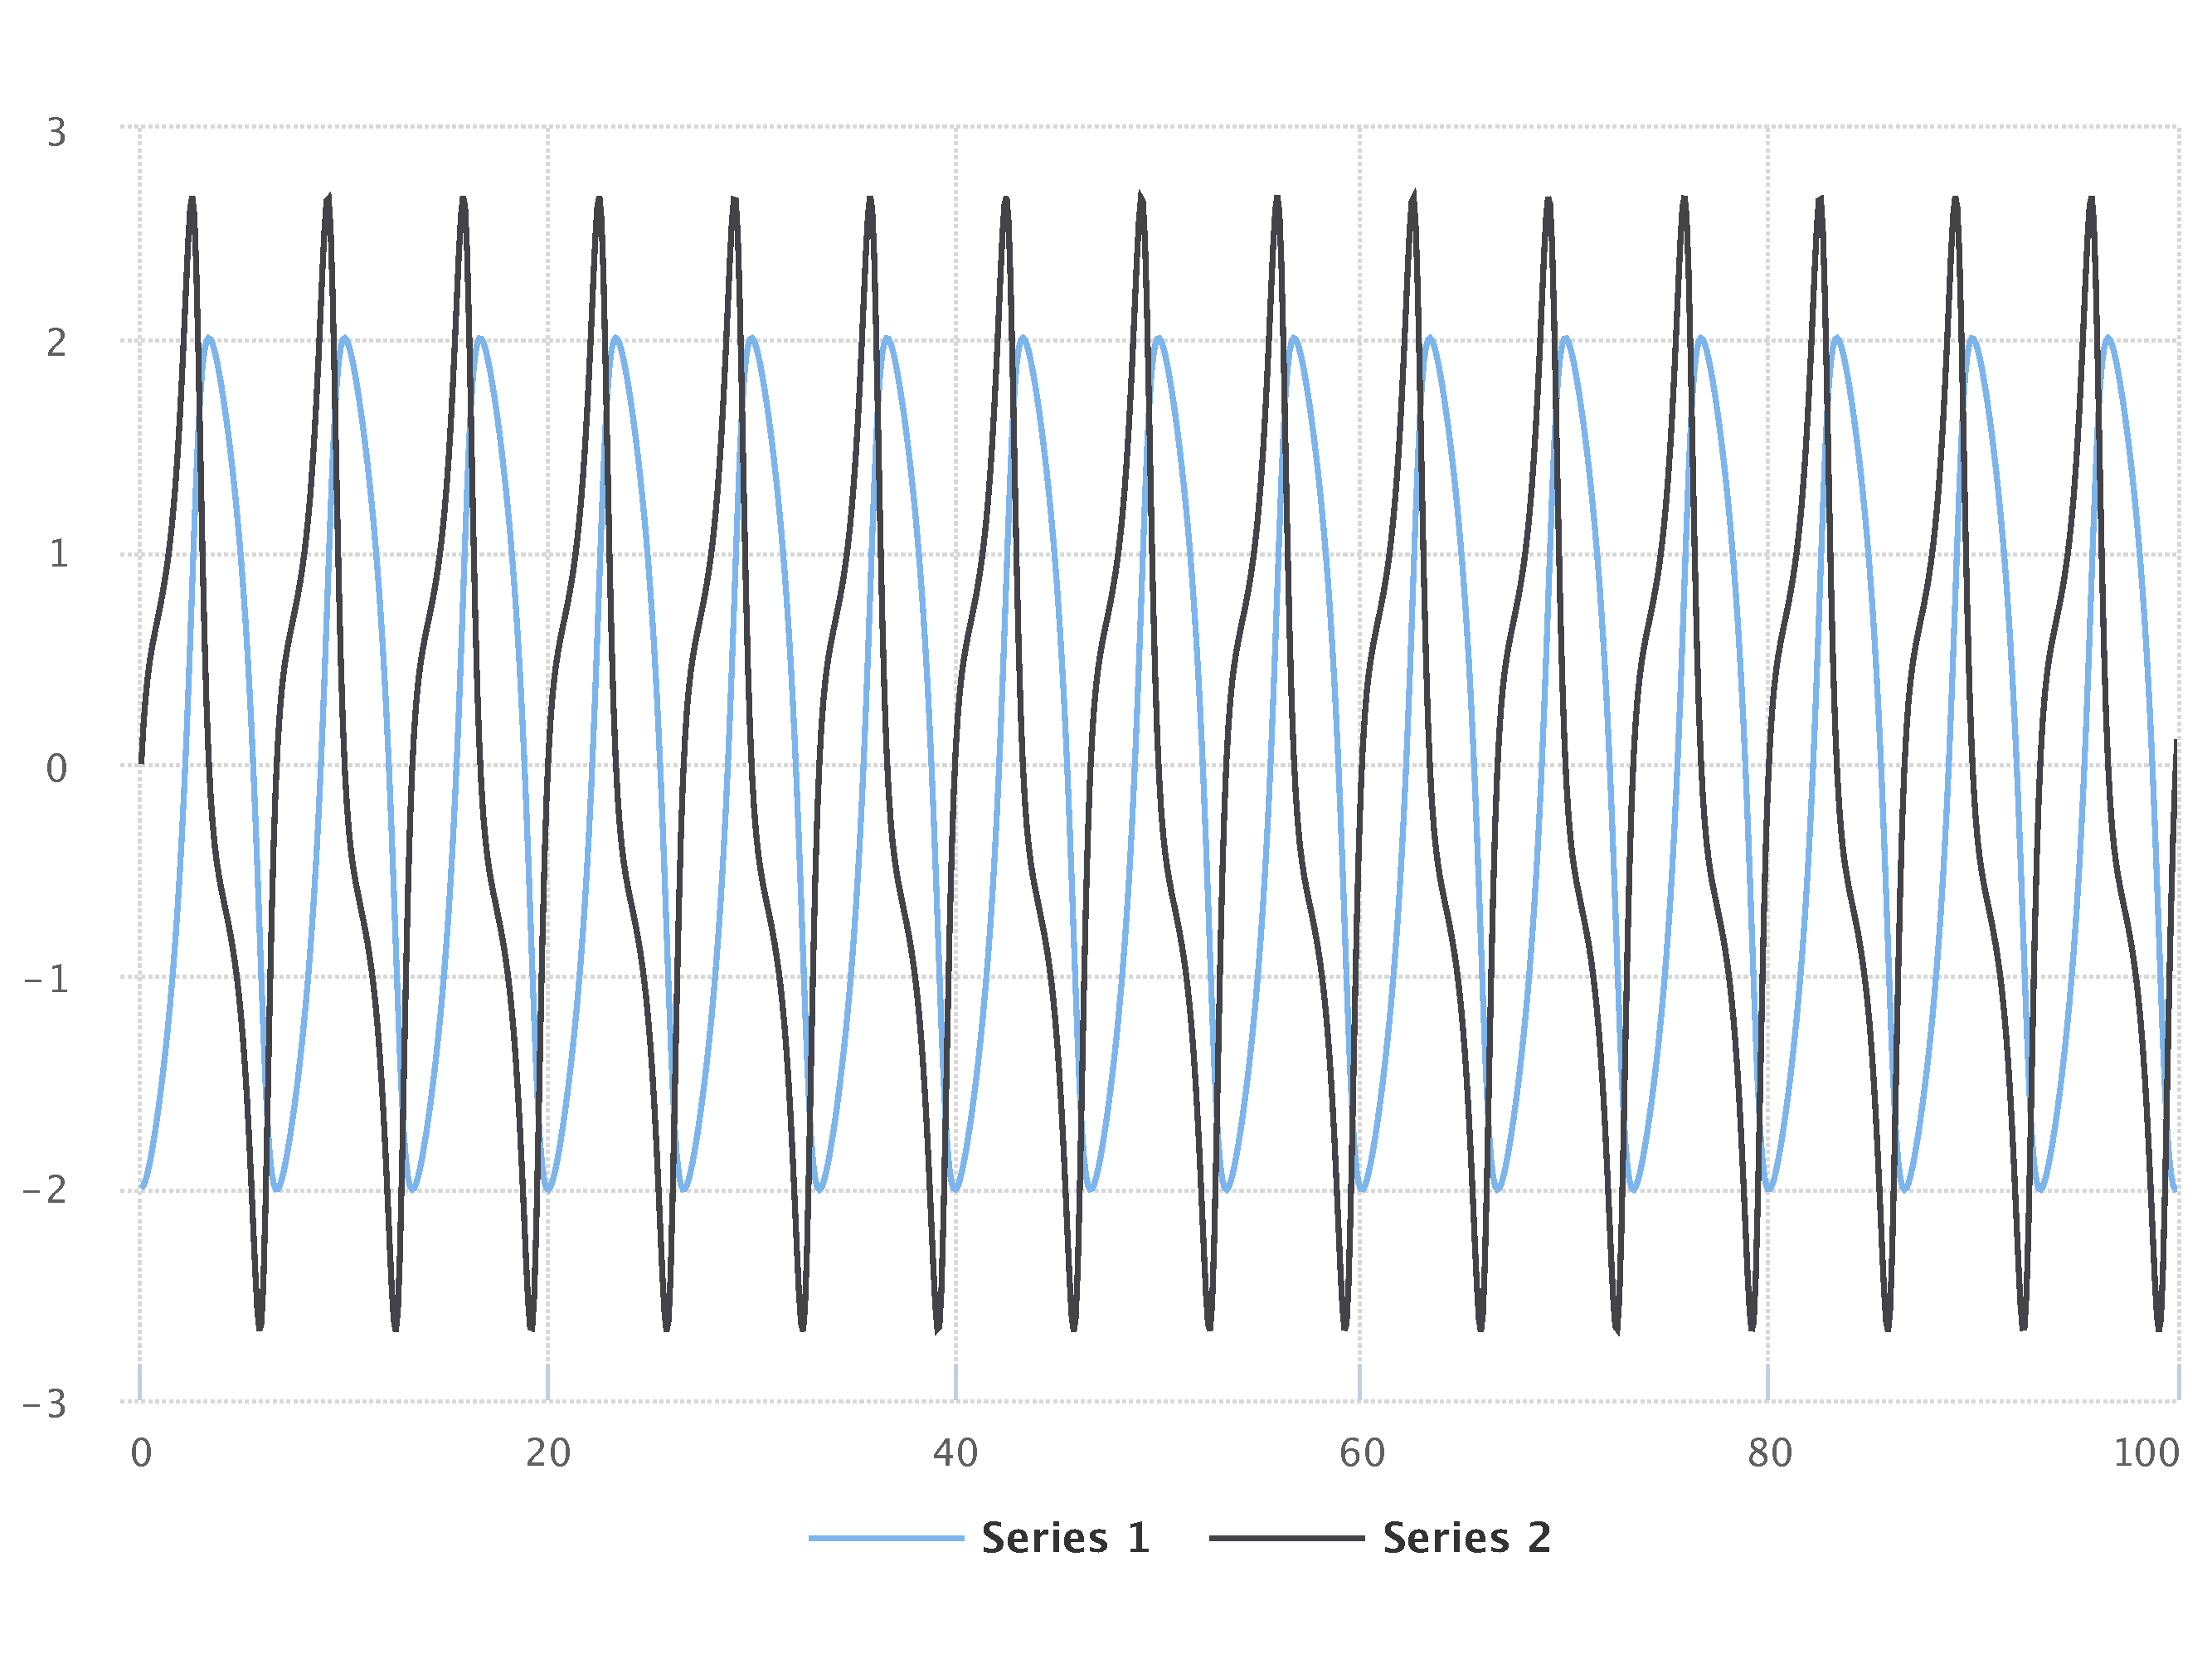
\includegraphics[width=1.0\textwidth]{examples/vanderpol-sbml/results/sedml_webtools/plot1}
        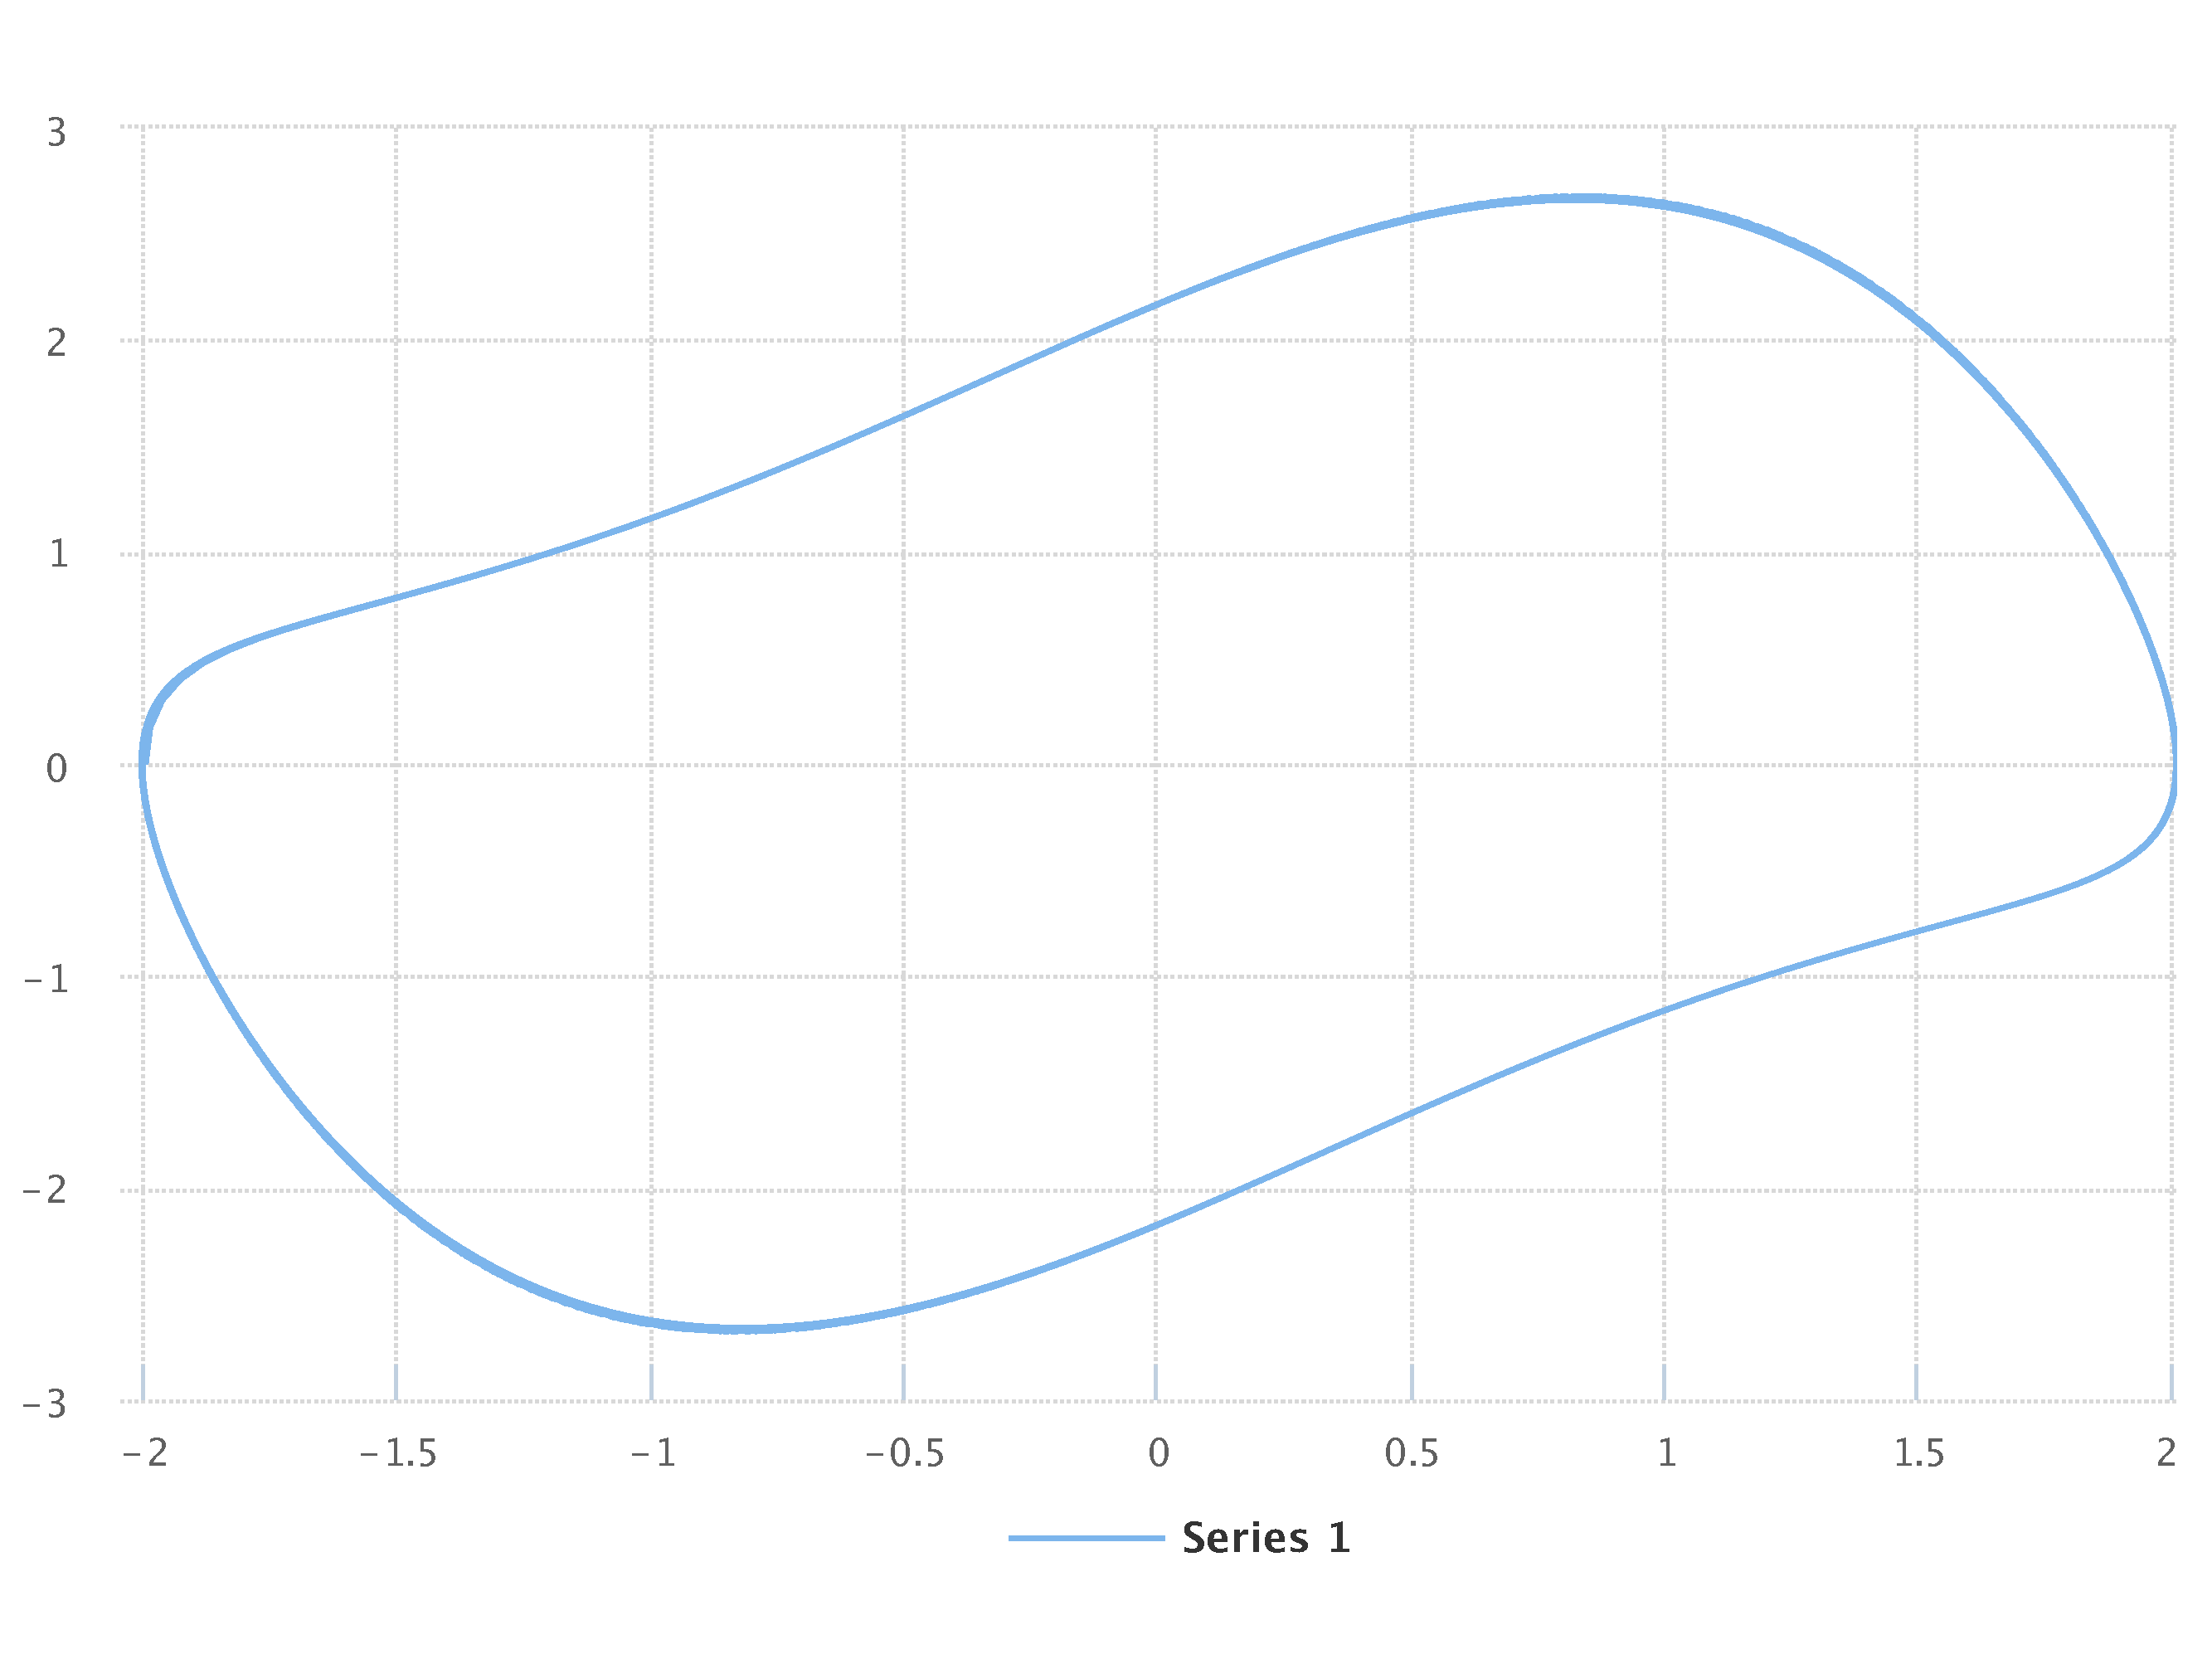
\includegraphics[width=1.0\textwidth]{examples/vanderpol-sbml/results/sedml_webtools/plot2}
        \caption{The simulation result gained from the simulation description given in \lst{vanderpol-sbml}. Simulation with SED-ML web tools \citep{bergmann2017sed}.}
    \end{minipage}\hfill
    \begin{minipage}{0.47\textwidth}
        \centering
        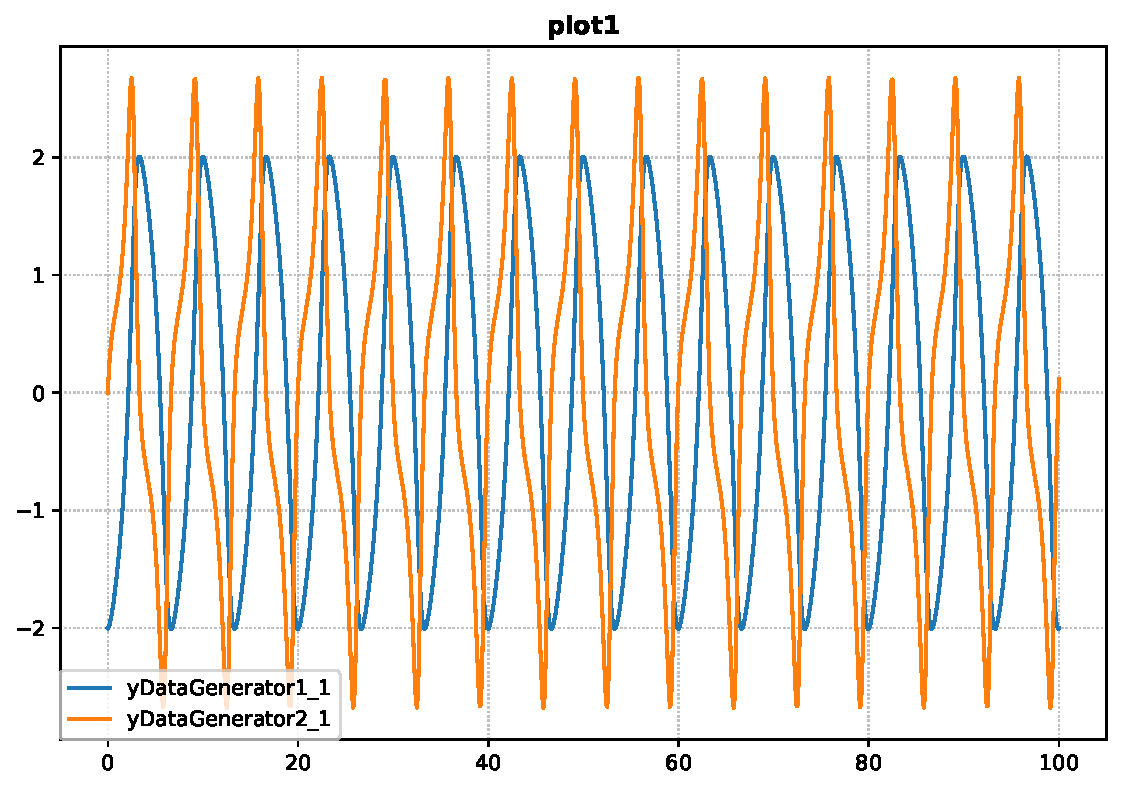
\includegraphics[width=1.0\textwidth]{examples/vanderpol-sbml/results/tellurium/plot1}
        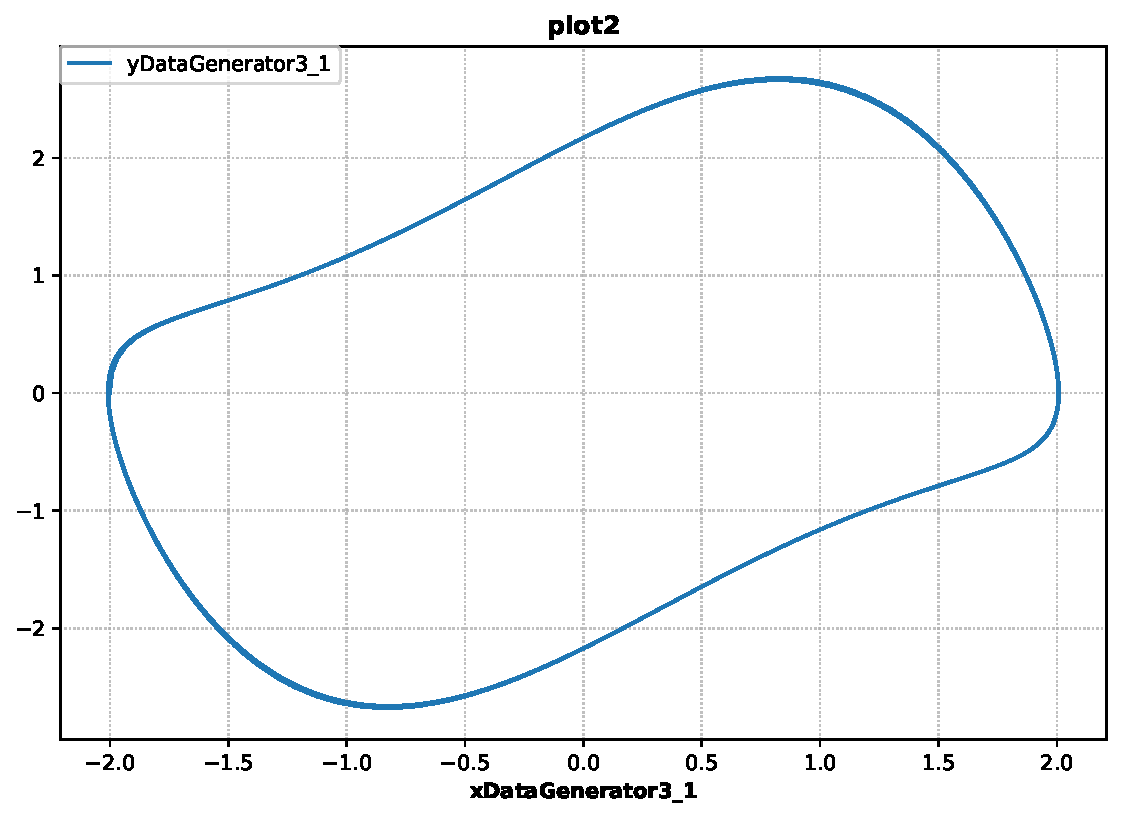
\includegraphics[width=1.0\textwidth]{examples/vanderpol-sbml/results/tellurium/plot2}
        \caption{Simulation with tellurium \citep{tellurium}.}
    \end{minipage}
    \label{fig:lorenz-sbml}
\end{figure}

\myXmlImport{Van der Pol Model (SBML) Simulation Description in SED-ML}{lst:vanderpol-sbml}{examples/vanderpol-sbml/vanderpol.xml}

\subsection{Van der Pol oscillator in CellML (\texttt{L1V3\_vanderpol-cellml.omex})}
\label{example:vanderpol_cellml}
The following example provides a SED-ML description for the simulation of the Van der Pol model in CellML \citep{cuellar:2003}. The time-course and the behavior in the phase plane are plotted. The mathematical model and the performed simulation experiment are identical to Appendix~\ref{example:vanderpol_sbml}.  \changed{This document can be found at \url{https://sed-ml.org/examples/L1V3/L1V3_vanderpol-cellml/vanderpol.xml}, and an OMEX version at \url{https://sed-ml.org/examples/L1V3/L1V3_vanderpol-cellml.omex}.}

\begin{figure}[ht]
    \centering
    \begin{minipage}{0.47\textwidth}
        \centering
        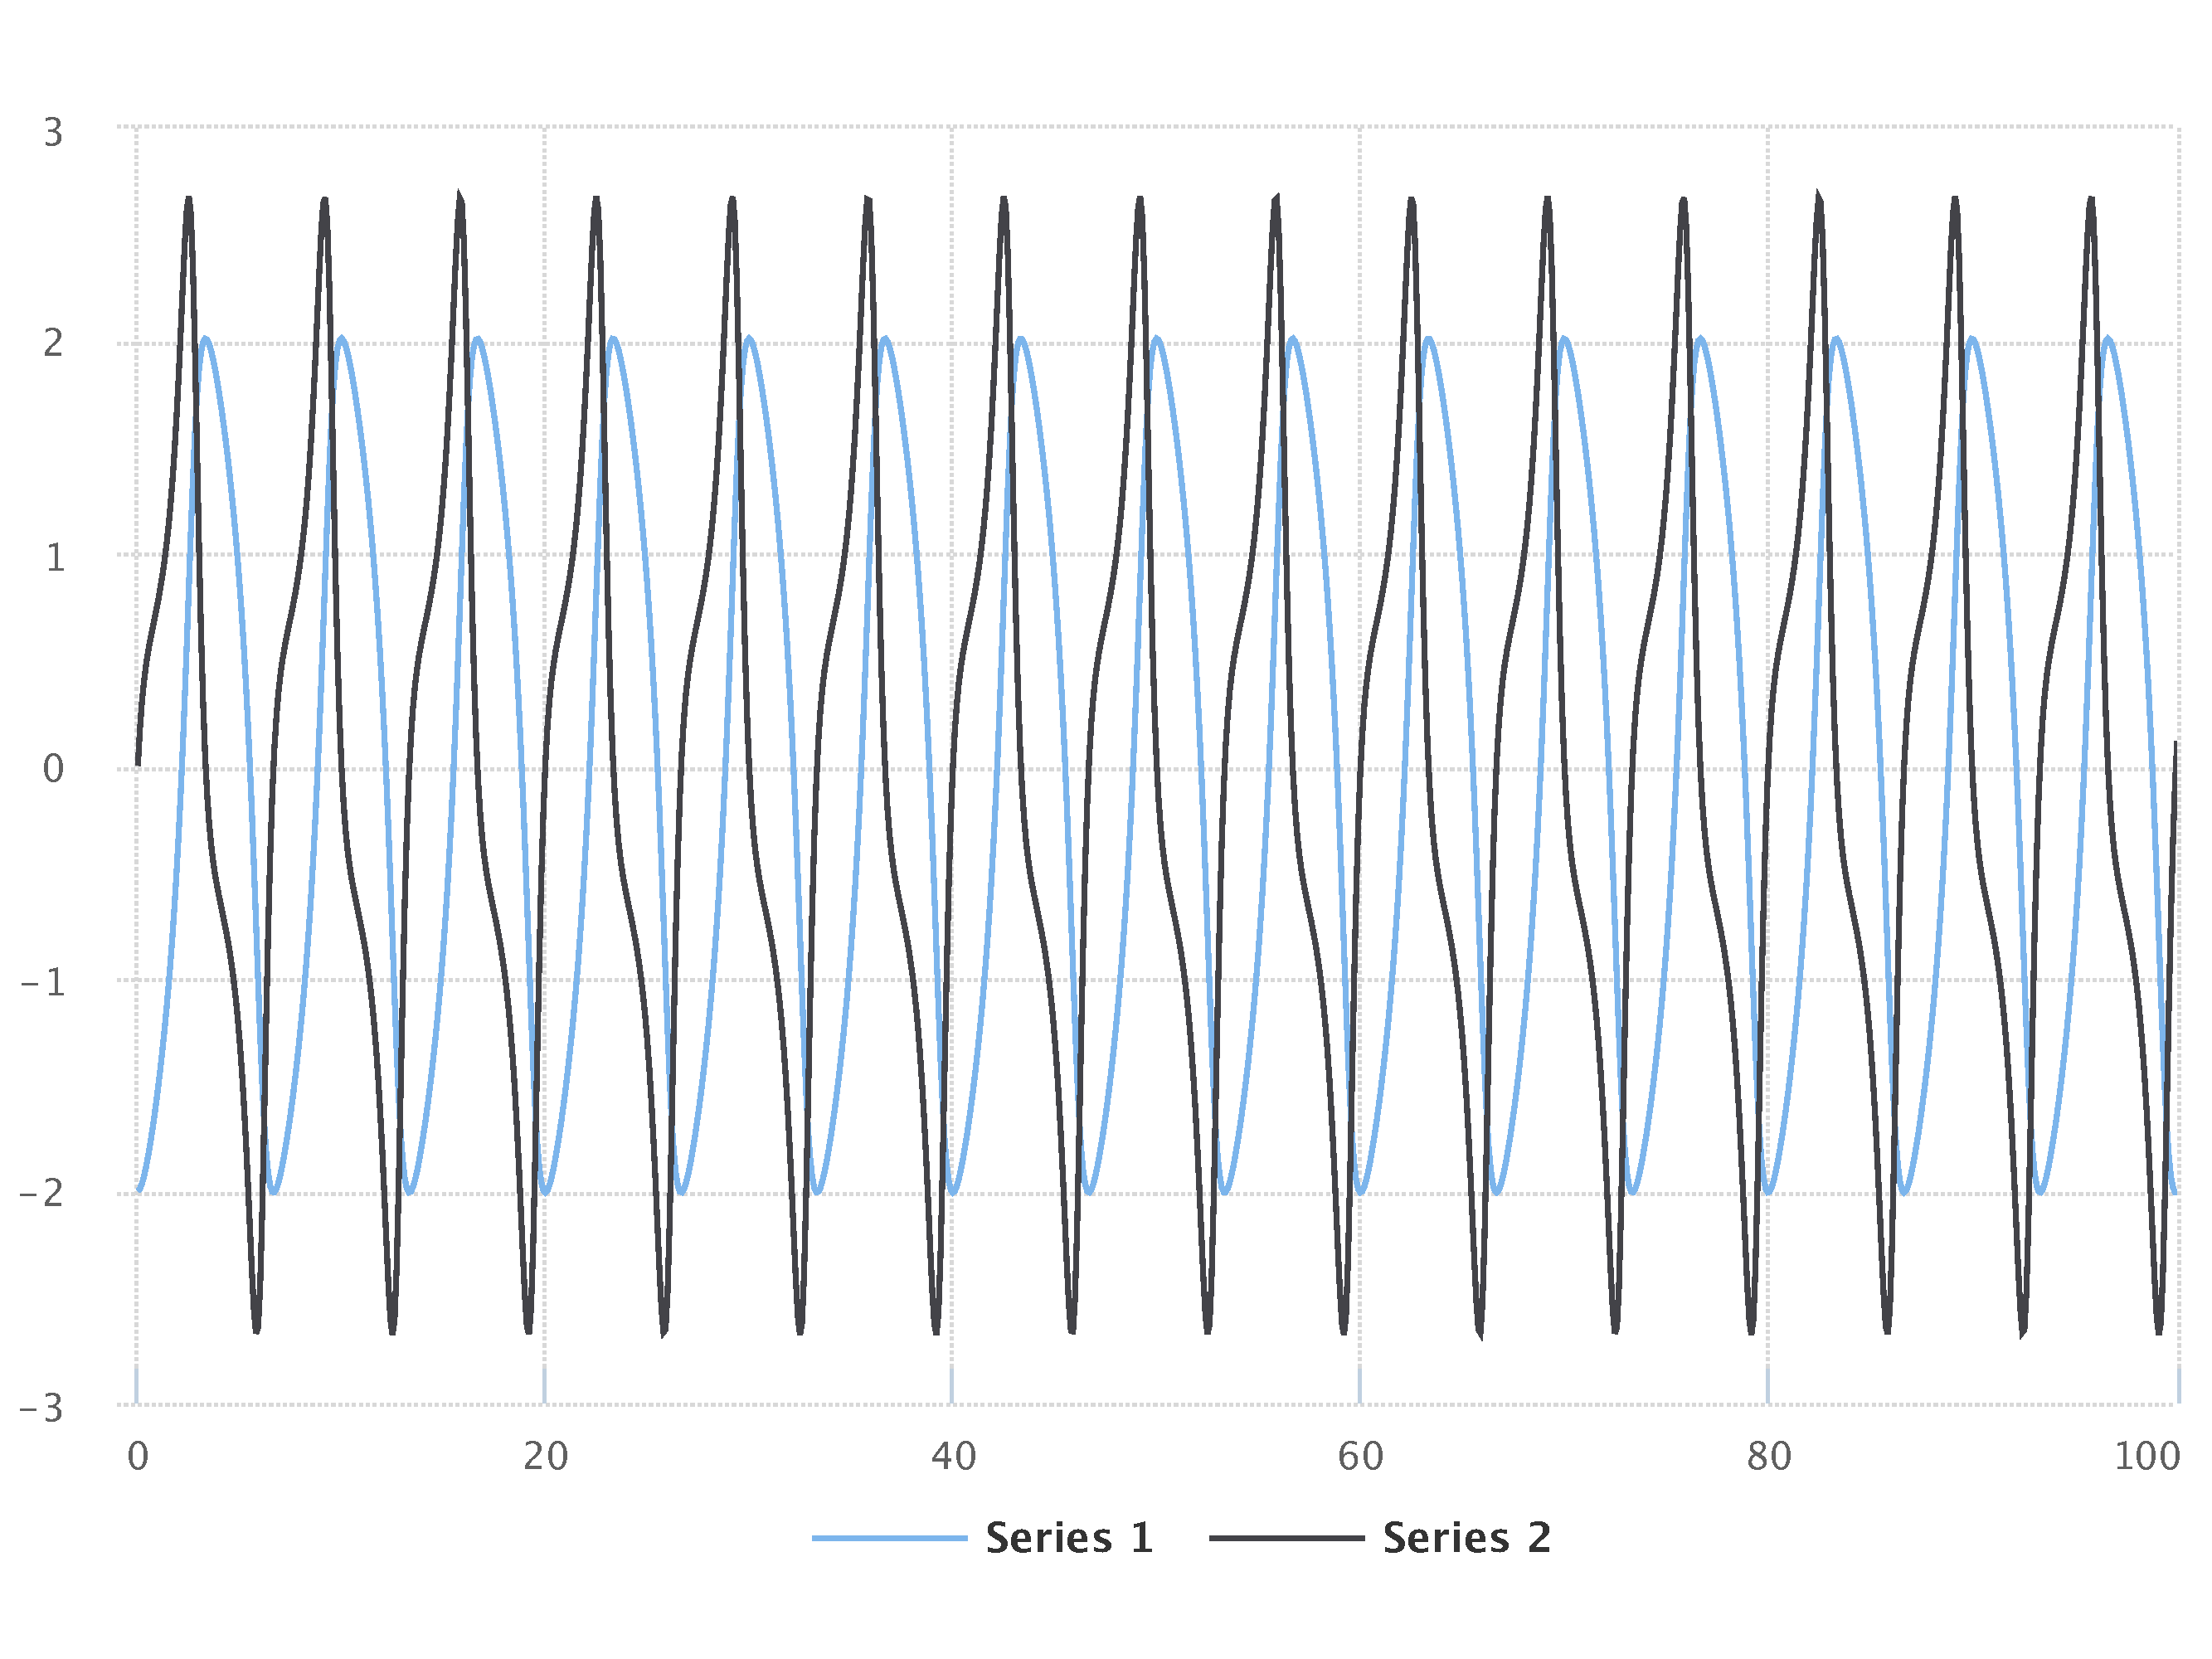
\includegraphics[width=1.0\textwidth]{examples/vanderpol-cellml/results/sedml_webtools/plot1}
        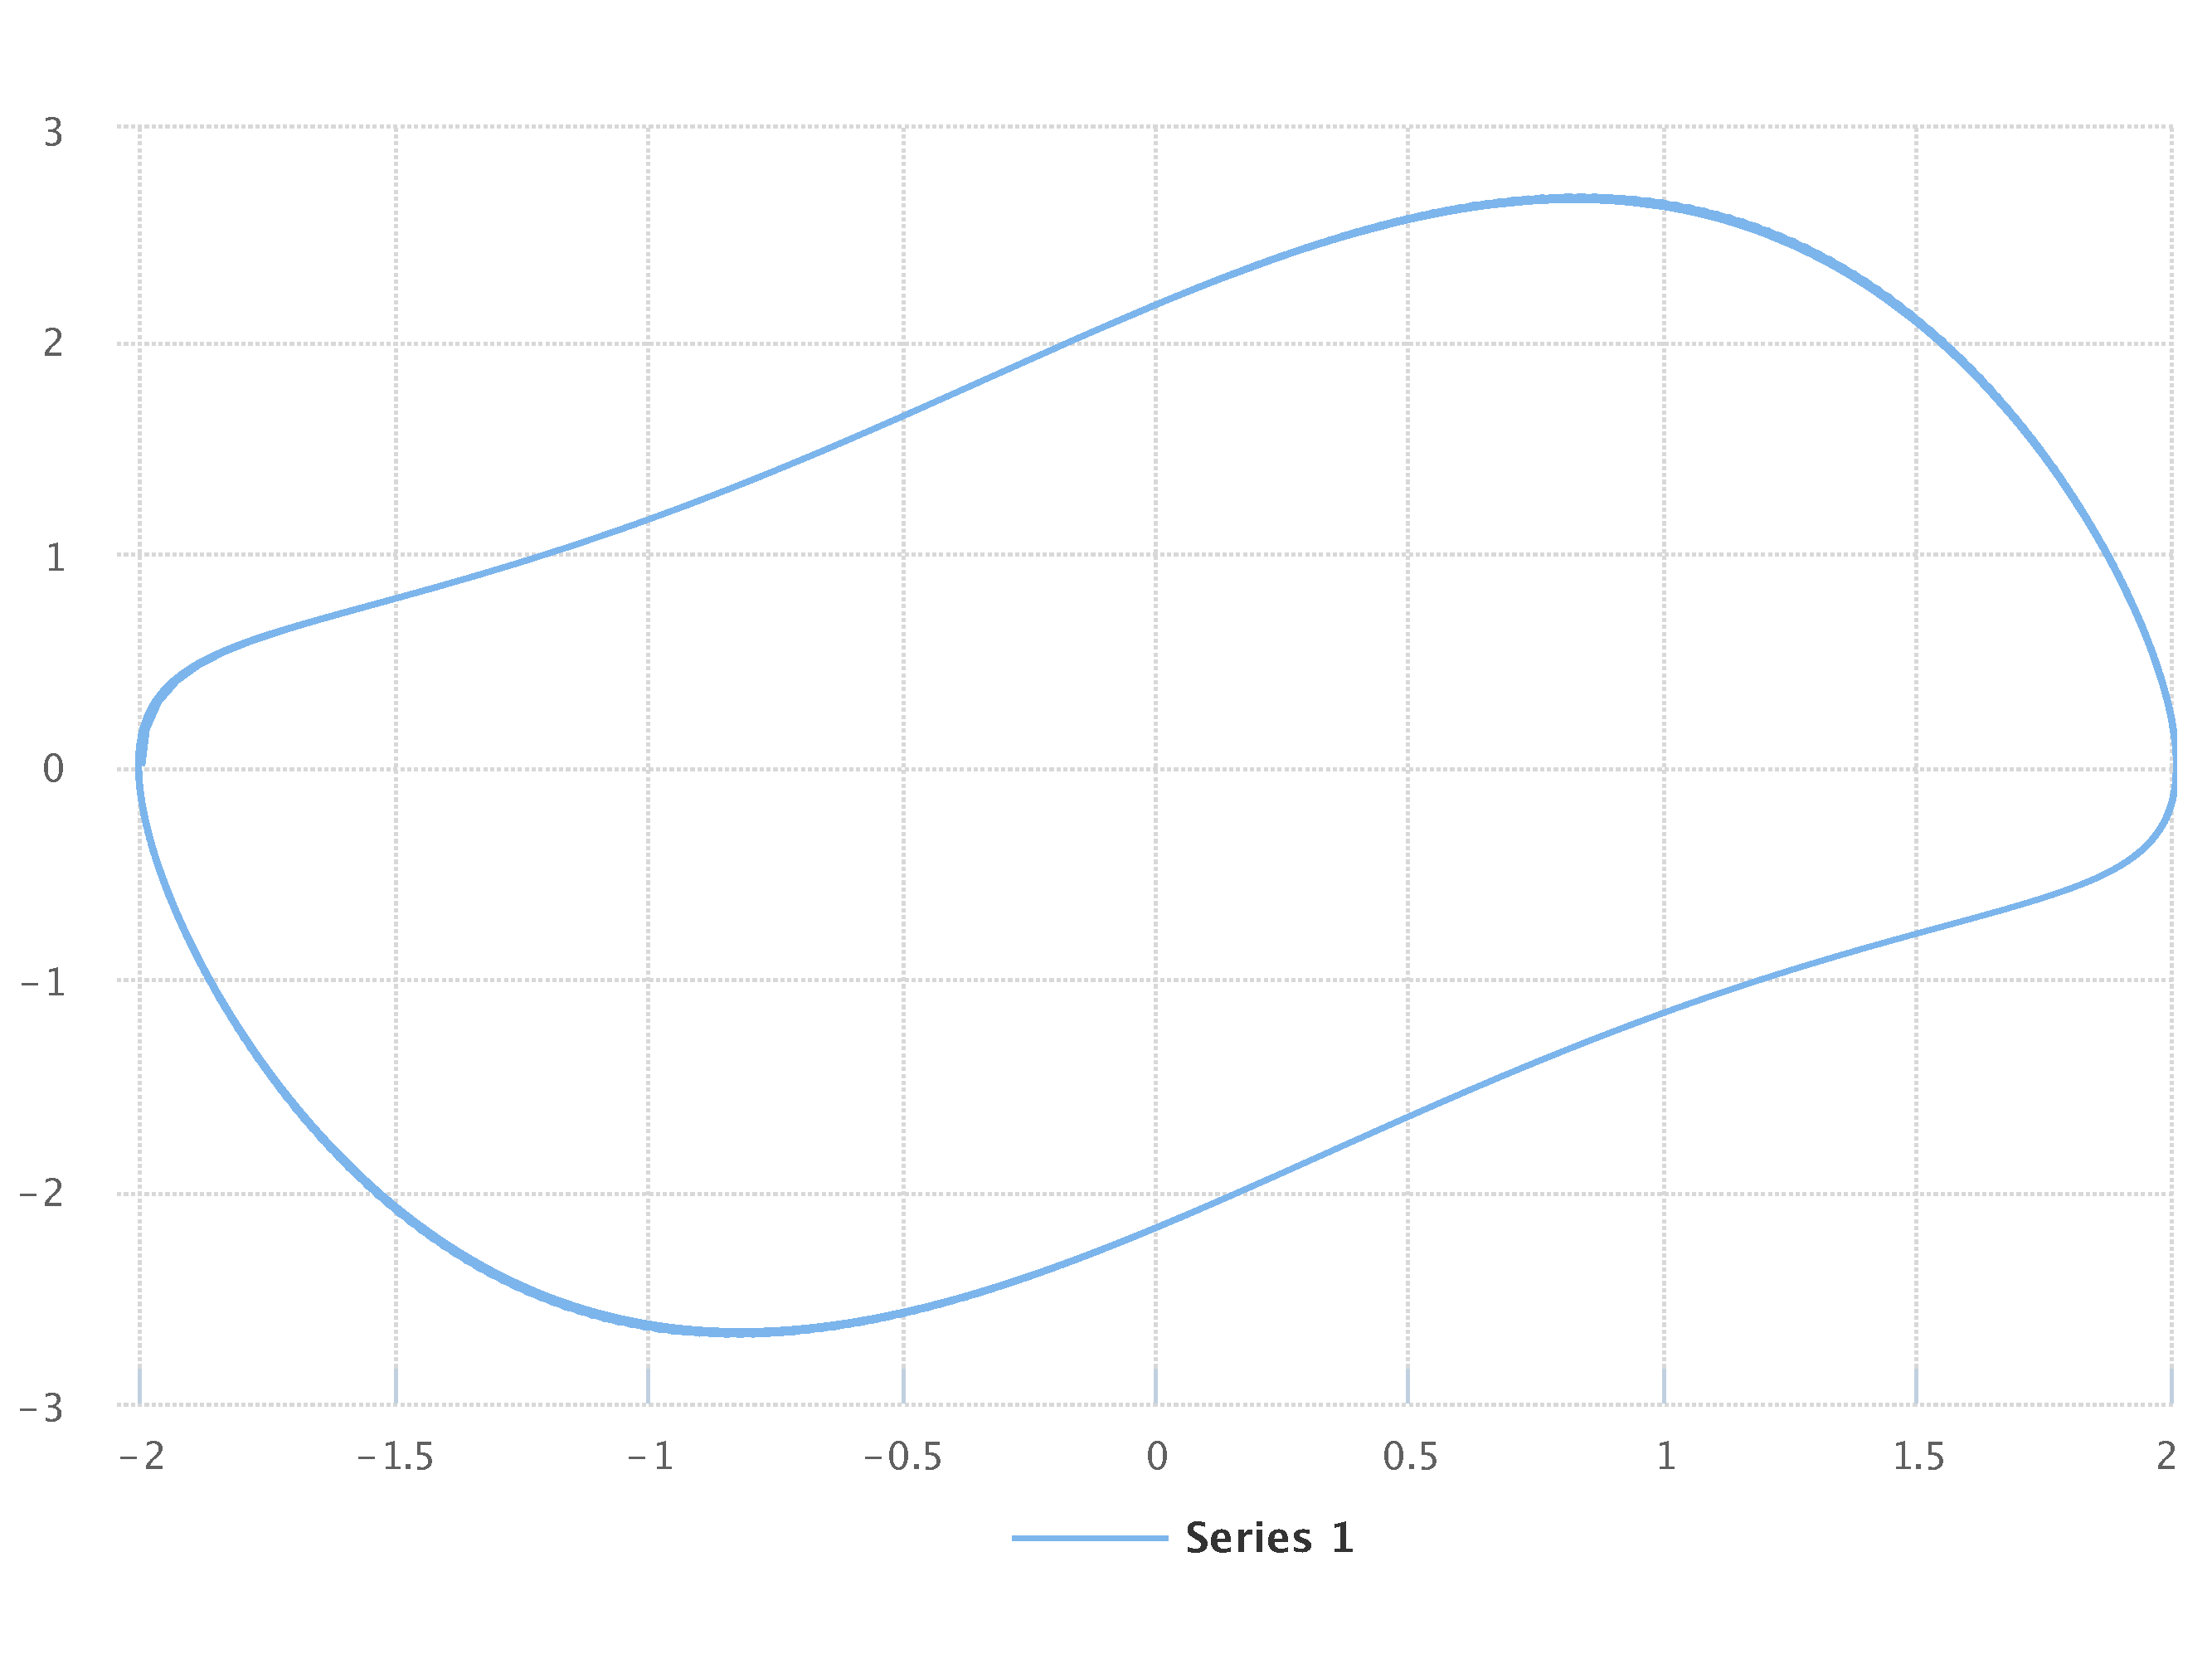
\includegraphics[width=1.0\textwidth]{examples/vanderpol-cellml/results/sedml_webtools/plot2}
        \caption{The simulation result gained from the simulation description given in \lst{vanderpol-cellml}. Simulation with SED-ML web tools \citep{bergmann2017sed}.}
    \end{minipage}\hfill
    \begin{minipage}{0.5\textwidth}
        \centering
        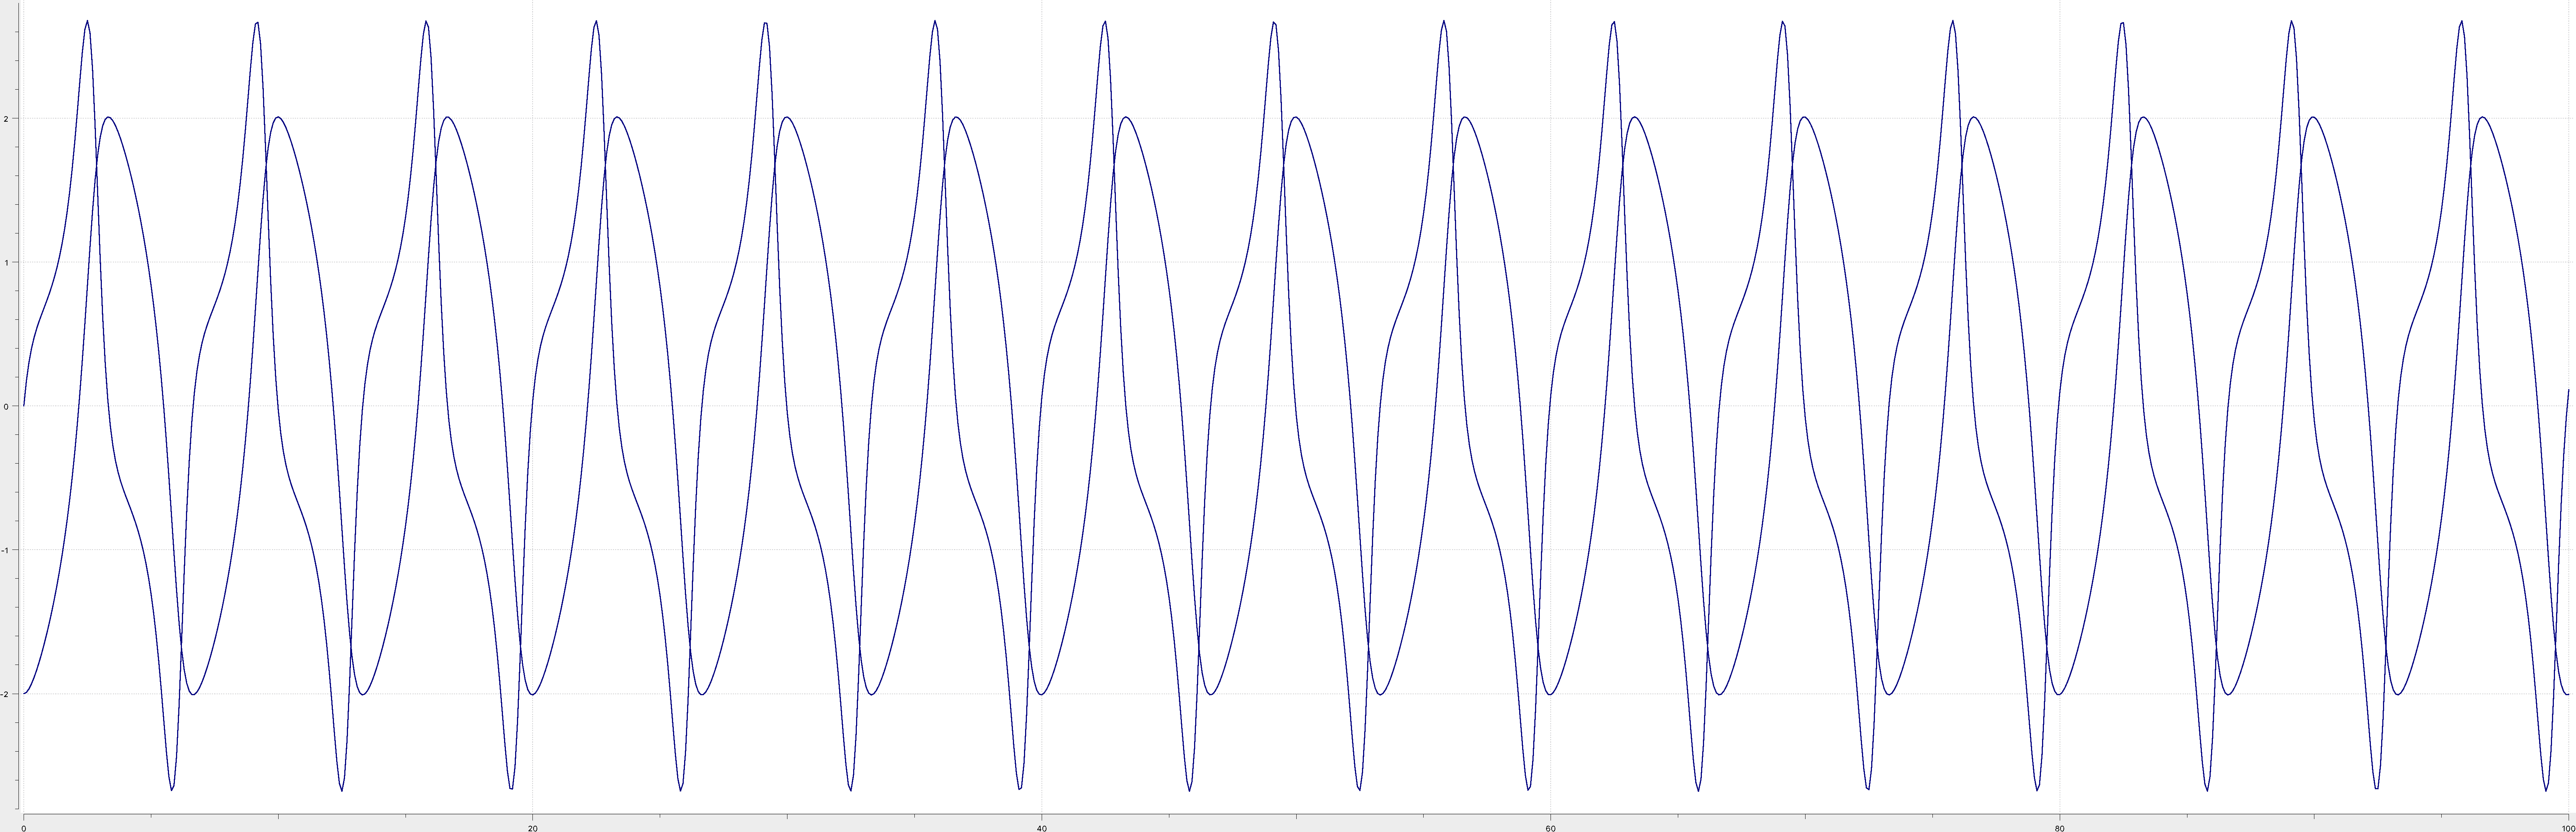
\includegraphics[width=1.0\textwidth]{examples/vanderpol-cellml/results/opencor/plot1}
        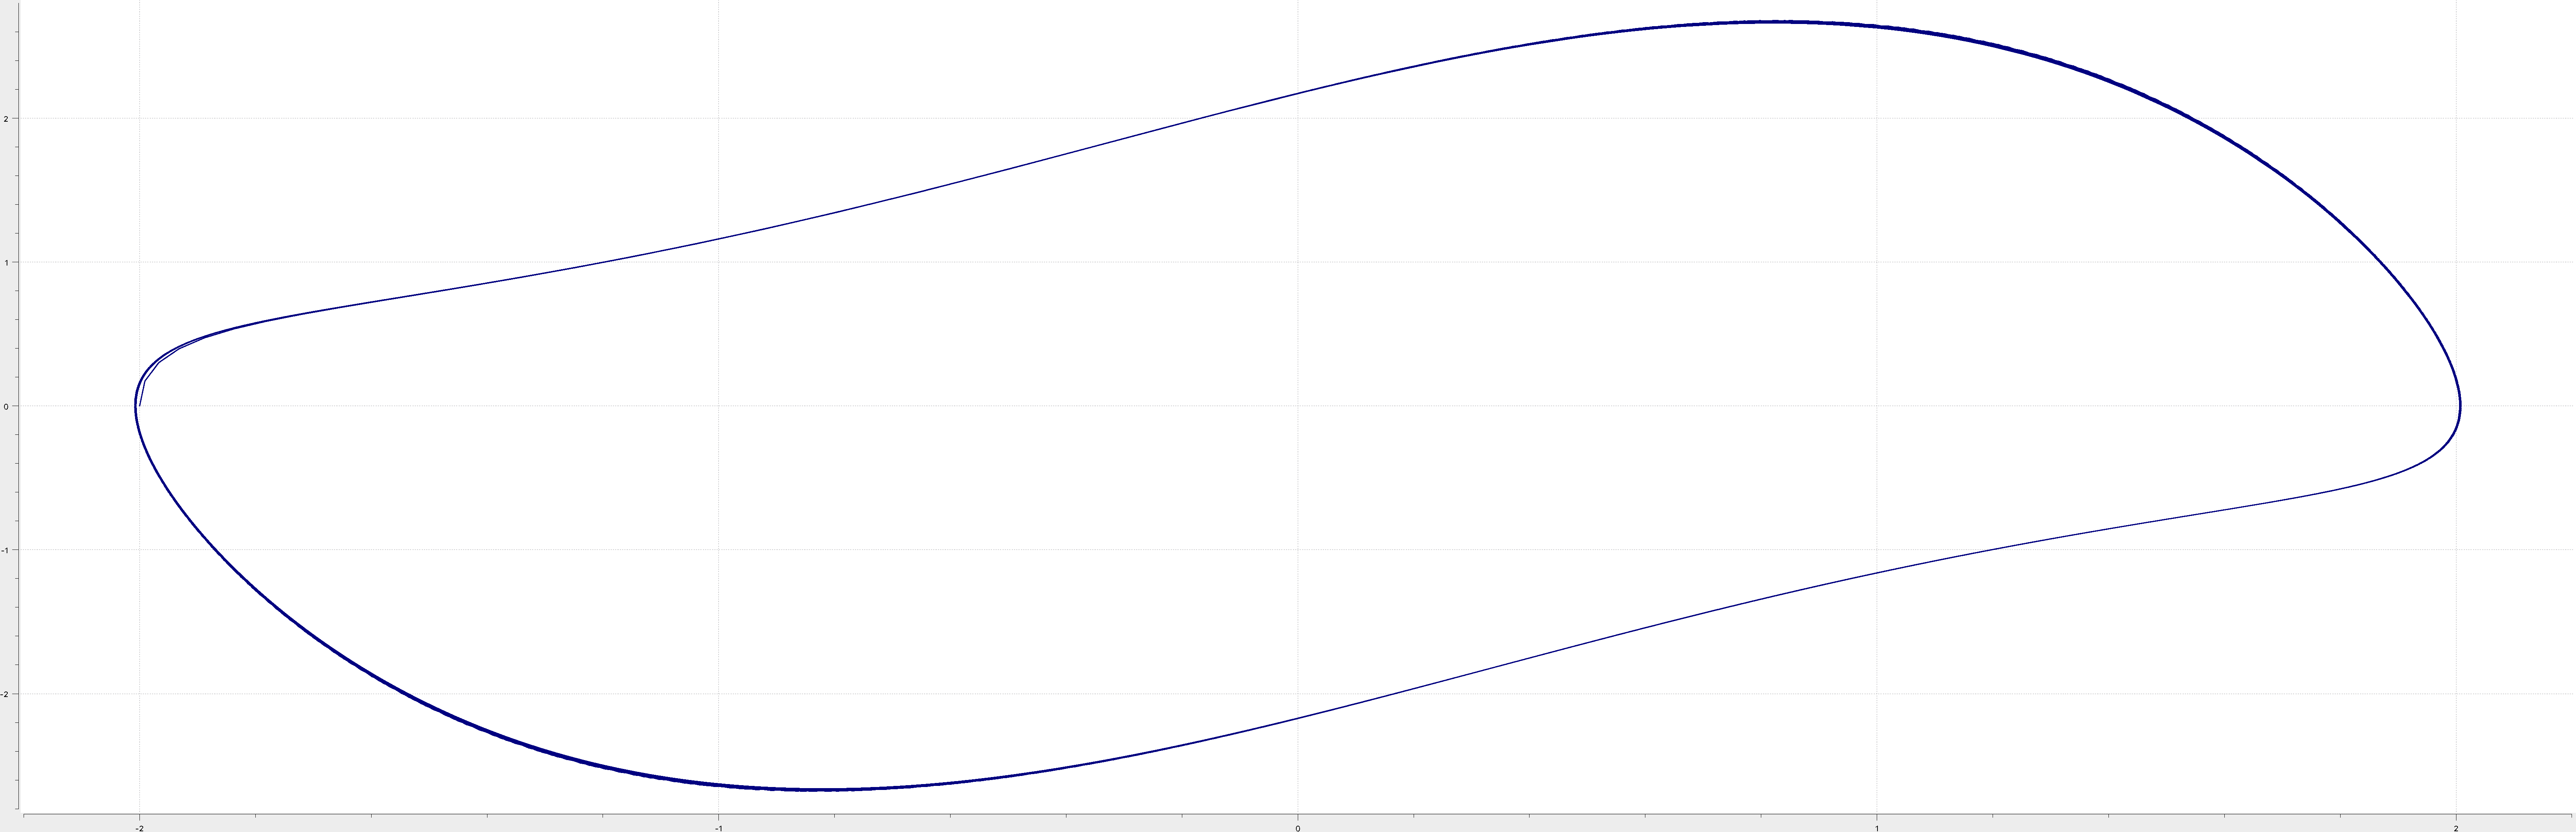
\includegraphics[width=1.0\textwidth]{examples/vanderpol-cellml/results/opencor/plot2}
        \caption{Simulation with OpenCOR \citep{garny2015opencor}.}
    \end{minipage}
    \label{fig:lorenz-cellml}
\end{figure}

\myXmlImport{Van der Pol Model (CellML) Simulation Description in SED-ML}{lst:vanderpol-cellml}{examples/vanderpol-cellml/vanderpol.xml}

% LORENZ EXAMPLES - DETERMINISTIC CHAOS
%\subsection{Lorenz Model SBML (\code{lorenz-sbml.omex})}
%\label{example:lorenz_sbml}
%The following example provides a SED-ML description for the simulation of the Lorenz model in SBML.
%
%\begin{figure}[ht]
%    \centering
%    \begin{minipage}{0.47\textwidth}
%        \centering
%        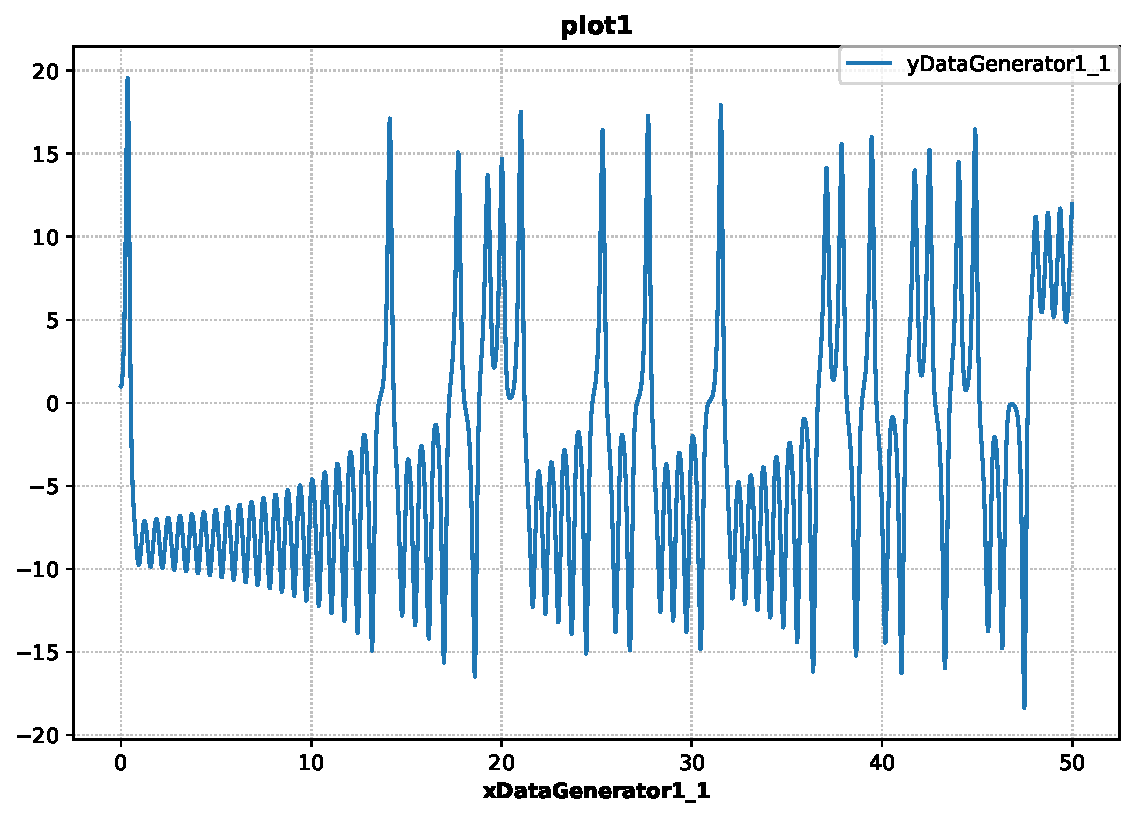
\includegraphics[width=1.0\textwidth]{examples/lorenz-sbml/results/sedml_webtools/plot1}
%        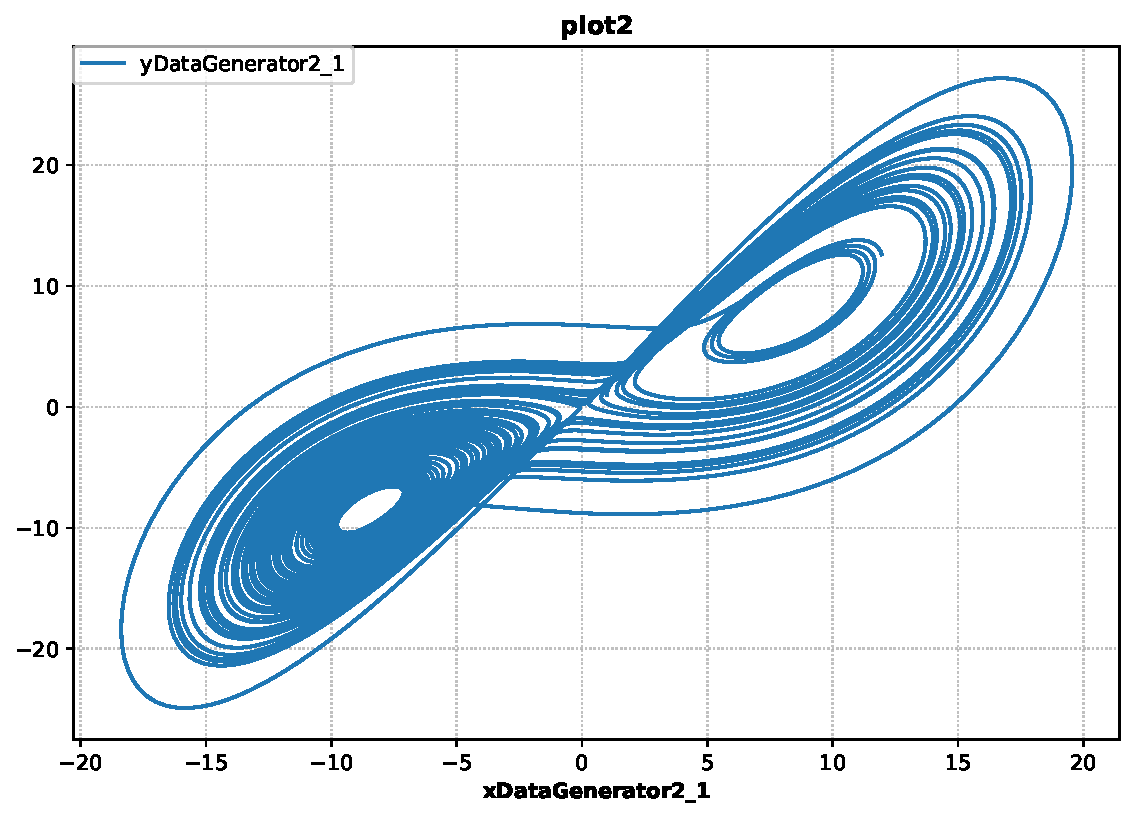
\includegraphics[width=1.0\textwidth]{examples/lorenz-sbml/results/sedml_webtools/plot2}
%		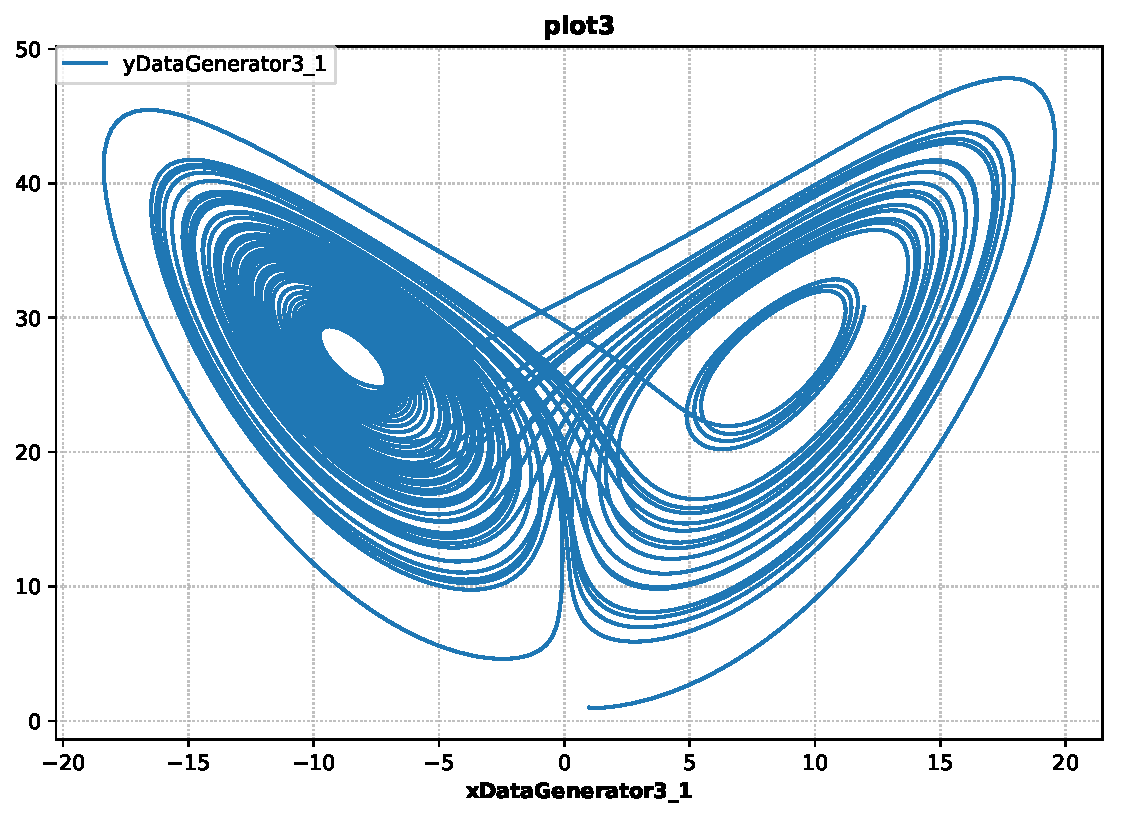
\includegraphics[width=1.0\textwidth]{examples/lorenz-sbml/results/sedml_webtools/plot3}
%        \caption{The simulation result gained from the simulation description given in \lst{lorenz-sbml}. Simulation with SED-ML web tools \citep{bergmann2017sed}.}
%    \end{minipage}\hfill
%    \begin{minipage}{0.47\textwidth}
%        \centering
%        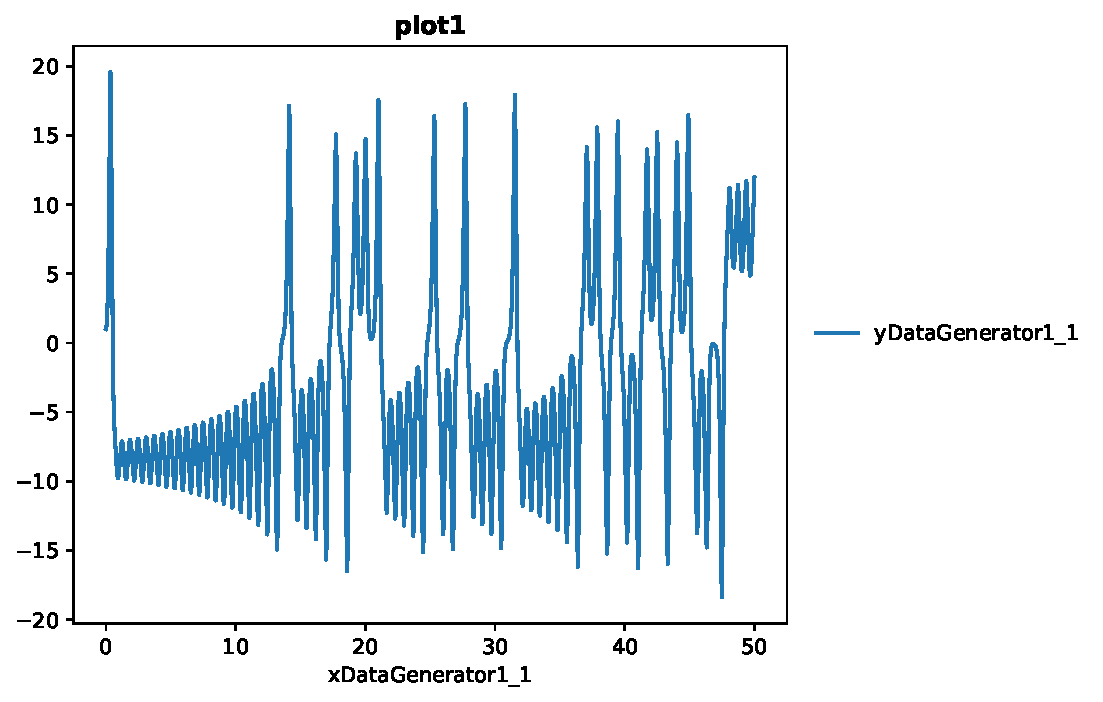
\includegraphics[width=1.0\textwidth]{examples/lorenz-sbml/results/tellurium/plot1}
%        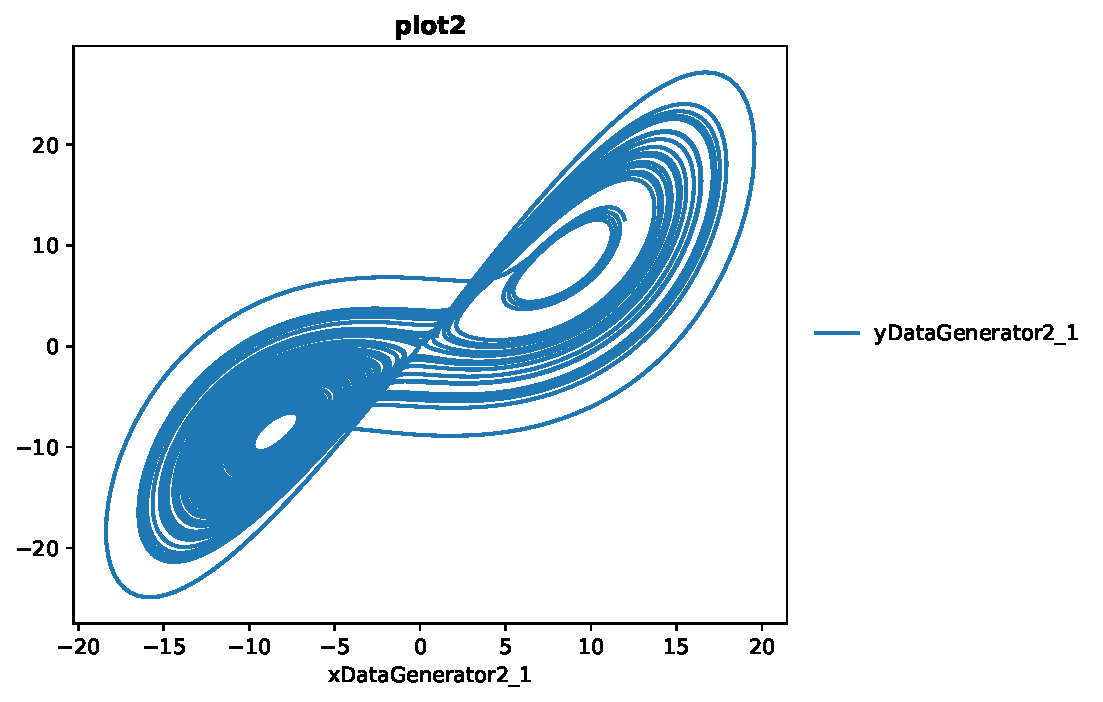
\includegraphics[width=1.0\textwidth]{examples/lorenz-sbml/results/tellurium/plot2}
%		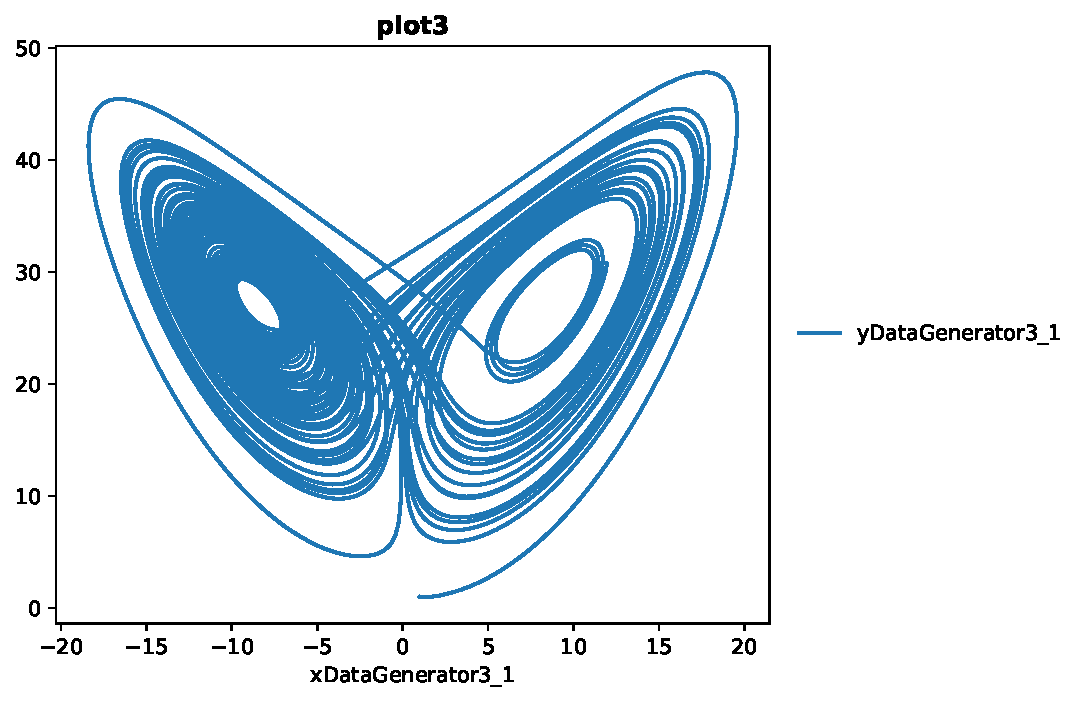
\includegraphics[width=1.0\textwidth]{examples/lorenz-sbml/results/tellurium/plot3}
%        \caption{Simulation with tellurium \citep{tellurium}.}
%    \end{minipage}
%    \label{fig:lorenz-sbml}
%\end{figure}
%
%\myXmlImport{LeLoup Model Simulation Description in SED-ML}{lst:lorenz-sbml}{examples/lorenz-sbml/lorenz.xml}
%
%\subsection{Lorenz Model CellML (\code{lorenz-cellml.omex})}
%\label{example:lorenz_cellml}
%The following example provides a SED-ML description for the simulation of the Lorenz model in CellML.
%
%\begin{figure}[ht]
%    \centering
%    \begin{minipage}{0.47\textwidth}
%        \centering
%        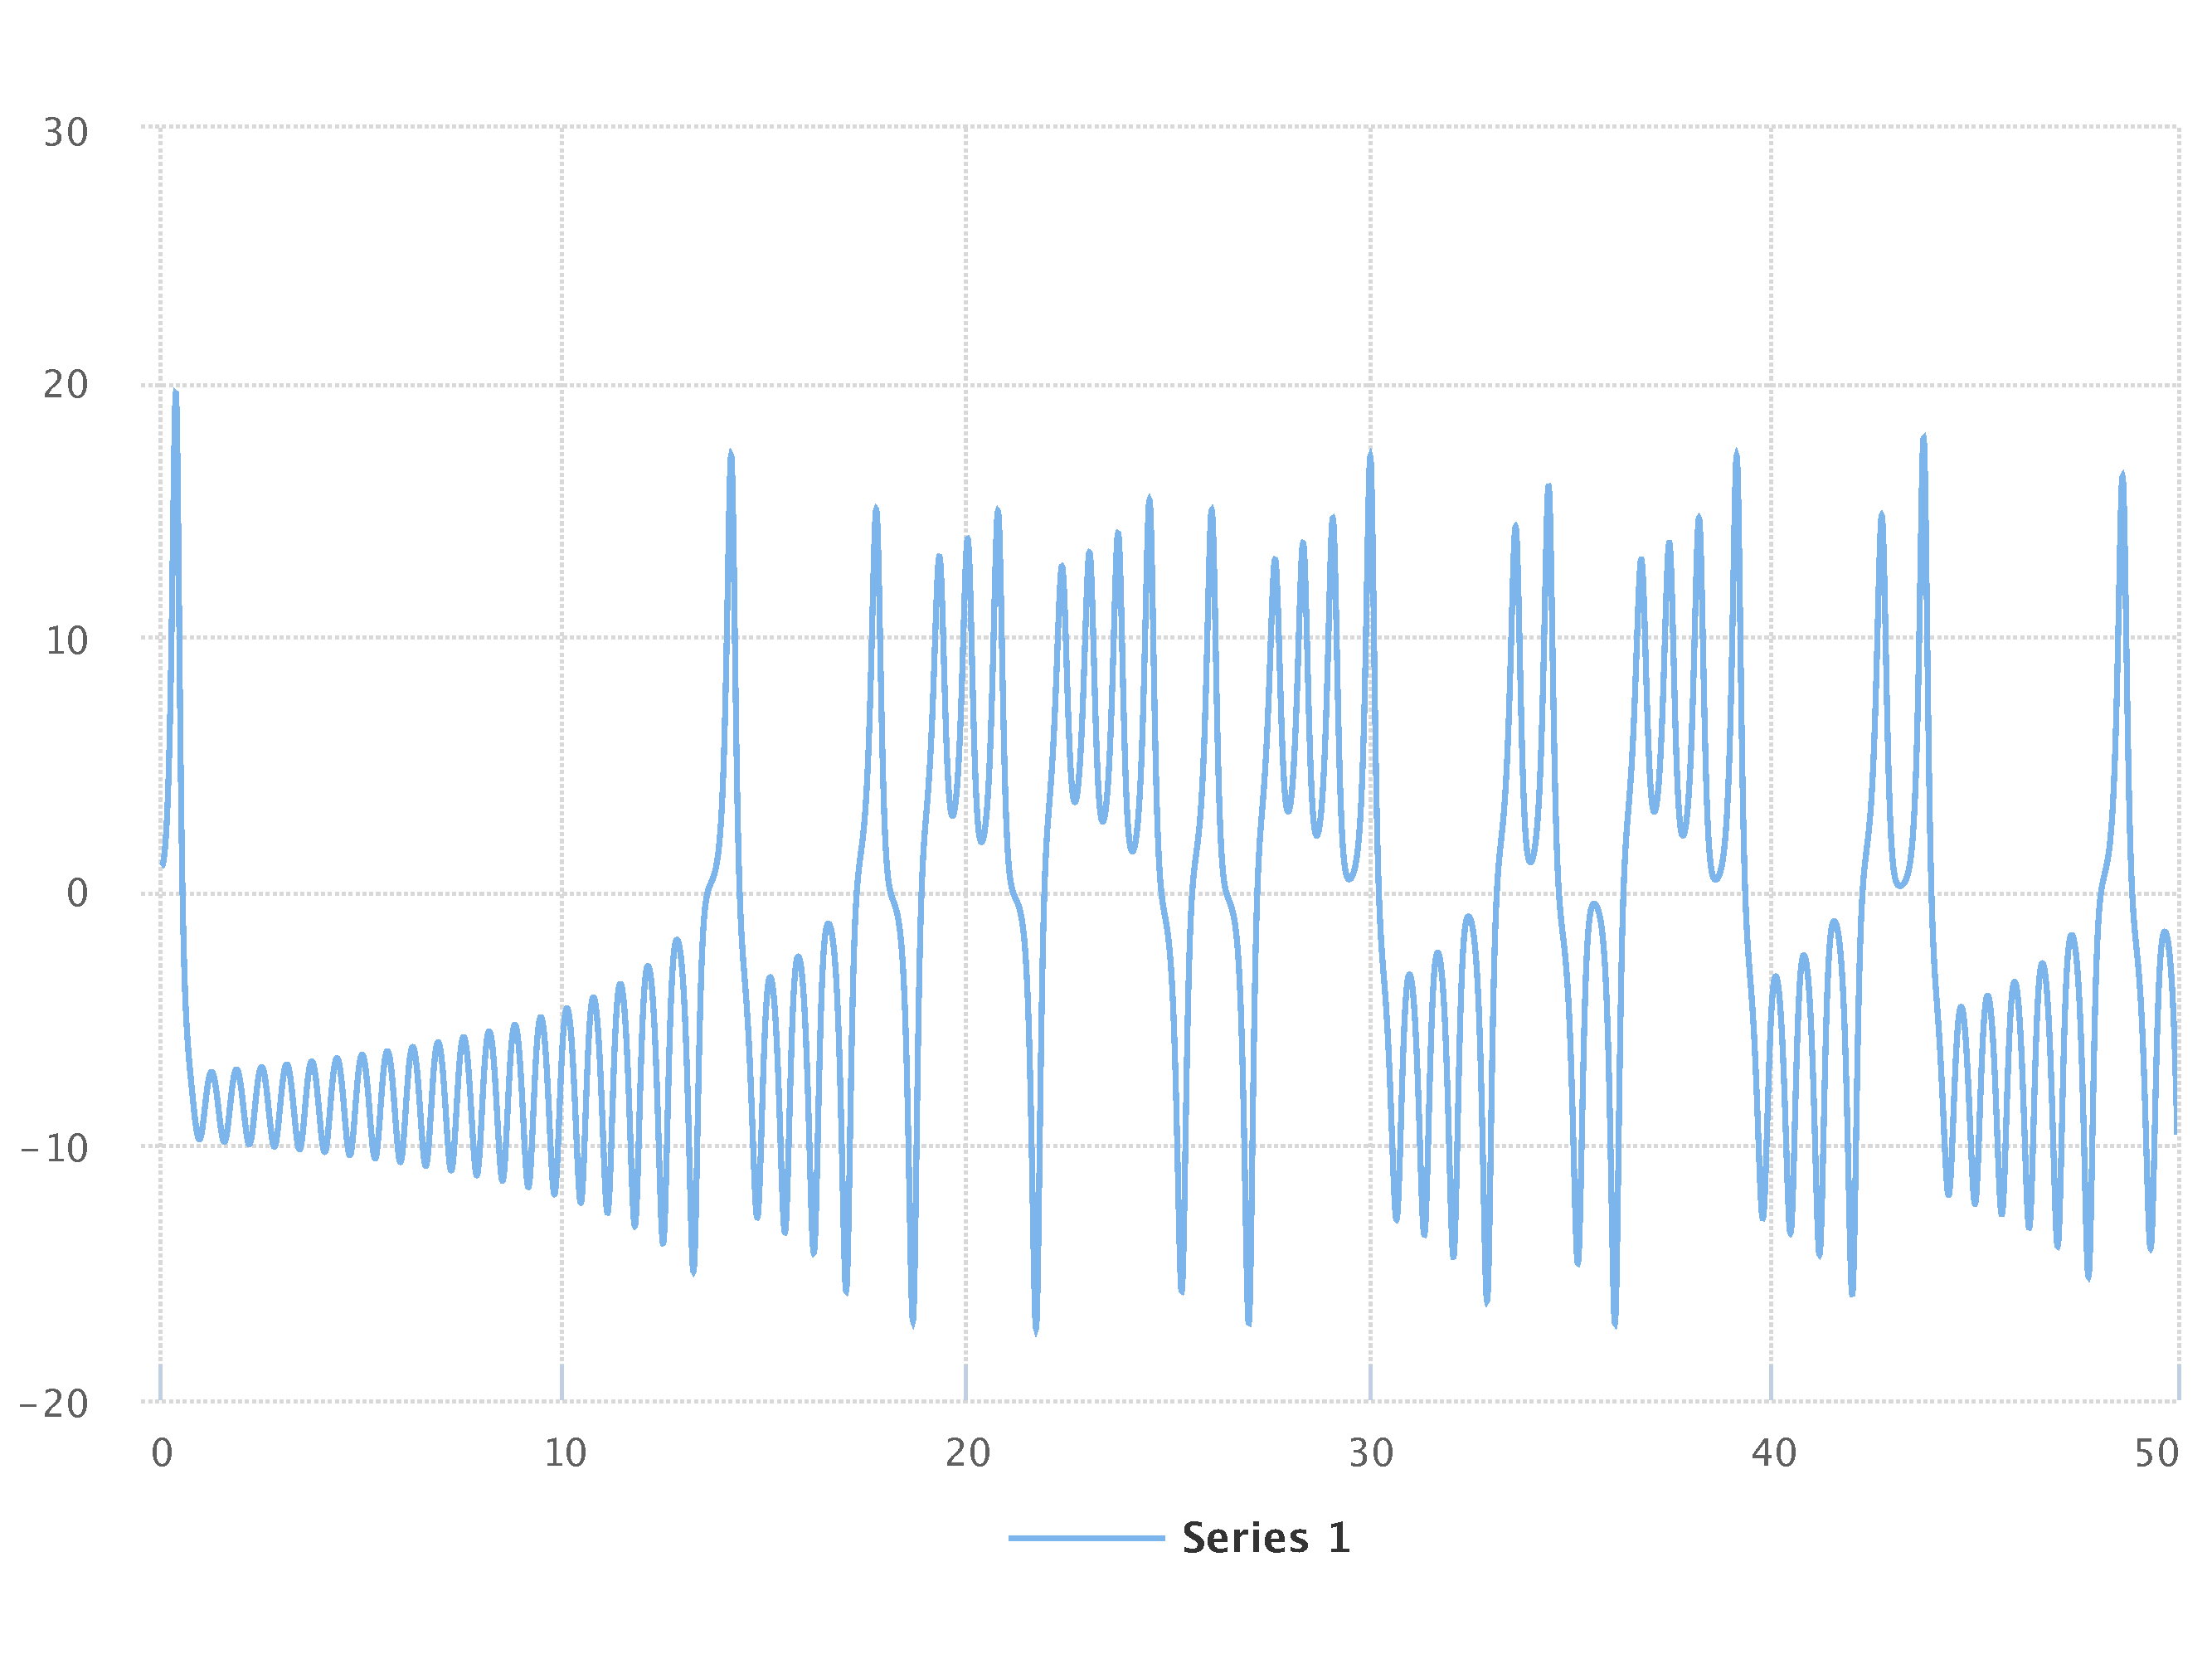
\includegraphics[width=1.0\textwidth]{examples/lorenz-cellml/results/sedml_webtools/plot1}
%        \caption{The simulation result gained from the simulation description given in \lst{lorenz-cellml}. Simulation with SED-ML web tools \citep{bergmann2017sed}.}
%    \end{minipage}\hfill
%    \begin{minipage}{0.47\textwidth}
%        \centering
%        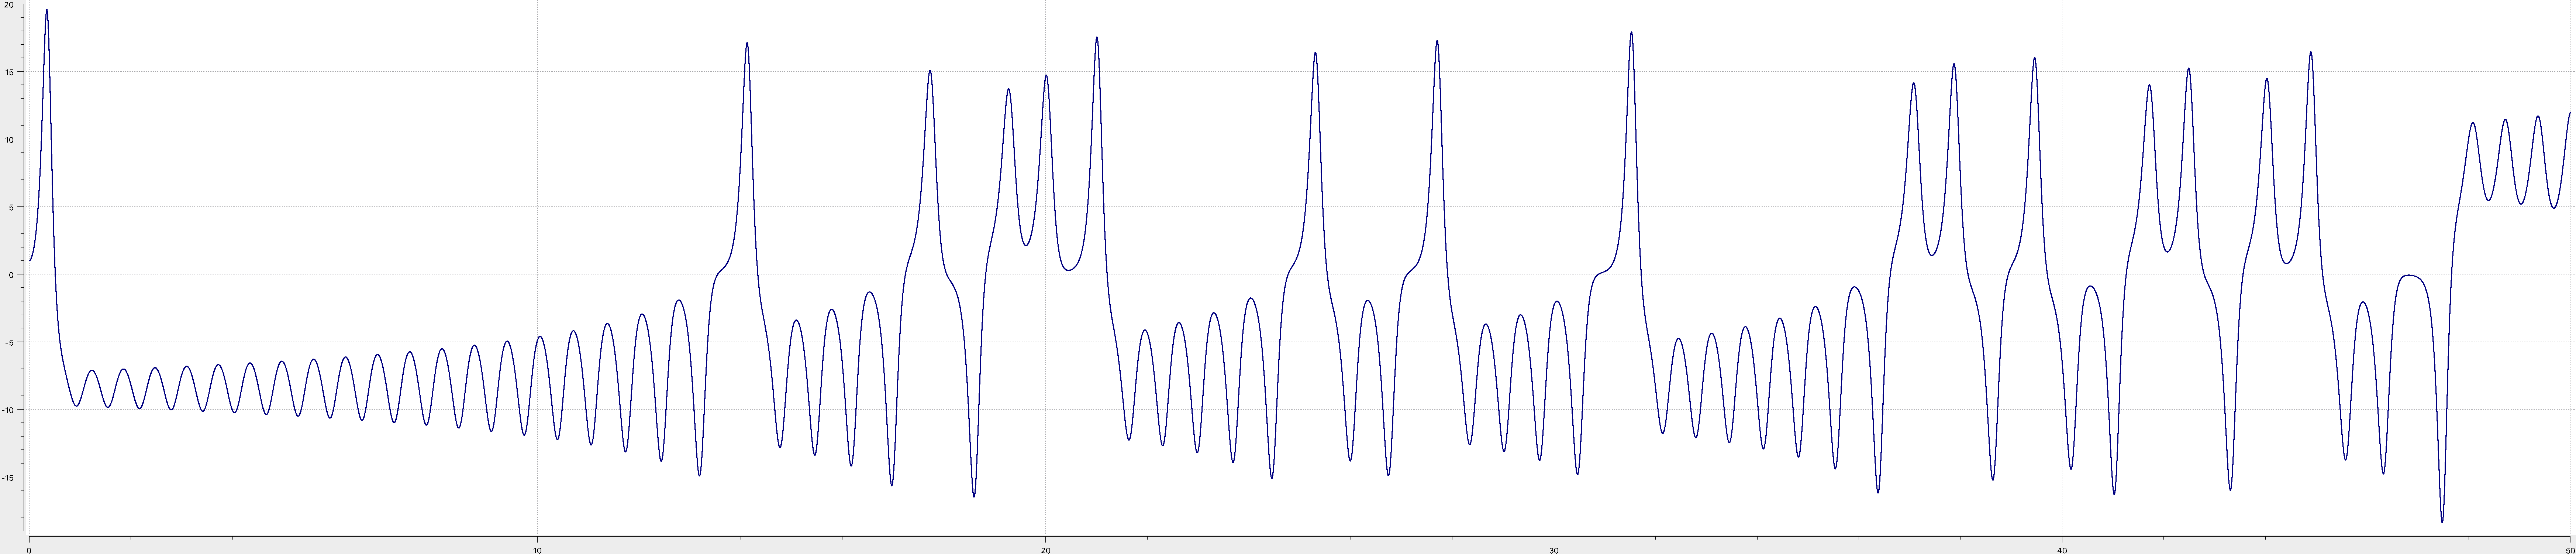
\includegraphics[width=1.0\textwidth]{examples/lorenz-cellml/results/opencor/plot1}
%        \caption{Simulation with OpenCOR \citep{garny2015opencor}.}
%    \end{minipage}
%    \label{fig:lorenz-cellml}
%\end{figure}
%
%\myXmlImport{LeLoup Model Simulation Description in SED-ML}{lst:lorenz-cellml}{examples/lorenz-cellml/lorenz.xml}

\pagebreak
% ~~~~~~~~~~~~~~~~~~~~~~~~~~~~~~~~~~~~
% REPRODUCING PUBLICATION RESULTS
% ~~~~~~~~~~~~~~~~~~~~~~~~~~~~~~~~~~~~
\section{Reproducing publication results}
SED-ML allows to describe simulation experiments from publications in a reproducible manner. This section provides such examples.

% ~~~ LE LOUP (SBML) ~~~
\subsection{Le Loup model (\texttt{L1V3\_leloup-sbml.omex})}
\label{example:leloup_sbml}
The following example provides a SED-ML description for the simulation of the model based on the publication \cite{LeLoup1999}.

The model is referenced by its SED-ML \hyperref[sec:id]{\element{id}} \code{model1} and refers to the model with the URL \url{https://www.ebi.ac.uk/biomodels/model/download/BIOMD0000000012.2?filename=BIOMD0000000012_url.xml}. A second model is defined in the example, using \code{model1} as a source and applying additional changes to it, in this case updating two model parameters.

One simulation setup is defined in the \code{listOfSimulations}. It is a \code{uniformTimeCourse} over 380 time units, providing 1000 output points. The algorithm used is the CVODE solver, as denoted by the KiSAO ID \code{KiSAO:0000019}.

A number of \hyperref[class:dataGenerator]{dataGenerators} are defined, which are the prerequisite for defining the simulation \hyperref[class:output]{output}. The first \hyperref[class:dataGenerator]{dataGenerator} with \hyperref[sec:id]{\element{id}} \code{time} collects the simulation time. \code{tim1} maps on the \code{Mt} entity in the model that is used in \code{task1} which in the model \code{model1}. The dataGenerator named \code{\texttt{per\_tim1}} maps on the \code{Cn} entity in \code{model1}. Finally  the fourth and fifth dataGenerators map on the \code{Mt} and \code{\texttt{per\_tim}} entity respectively in the updated model with ID \code{model2}.

The \hyperref[class:output]{output} defined in the experiment consists of three \hyperref[class:plot2D]{2D plots}. The first plot has two \hyperref[class:curve]{curves} and provides the time course of the simulation using the tim mRNA concentrations from both tasks. The second plot shows the \code{\texttt{per\_tim}} concentration against the \code{tim} concentration for the oscillating model. The third plot shows the same plot for the chaotic model. The resulting three plots are depicted in Figure \ref{fig:leloup-sbml1} and \ref{fig:leloup-sbml2}.  \changed{This document can be found at \url{https://sed-ml.org/examples/L1V3/L1V3_leloup-sbml/leloup-sbml.xml}, and an OMEX version at \url{https://sed-ml.org/examples/L1V3/L1V3_leloup-sbml.omex}.}

\begin{figure}[ht]
    \centering
    \begin{minipage}{0.47\textwidth}
        \centering
        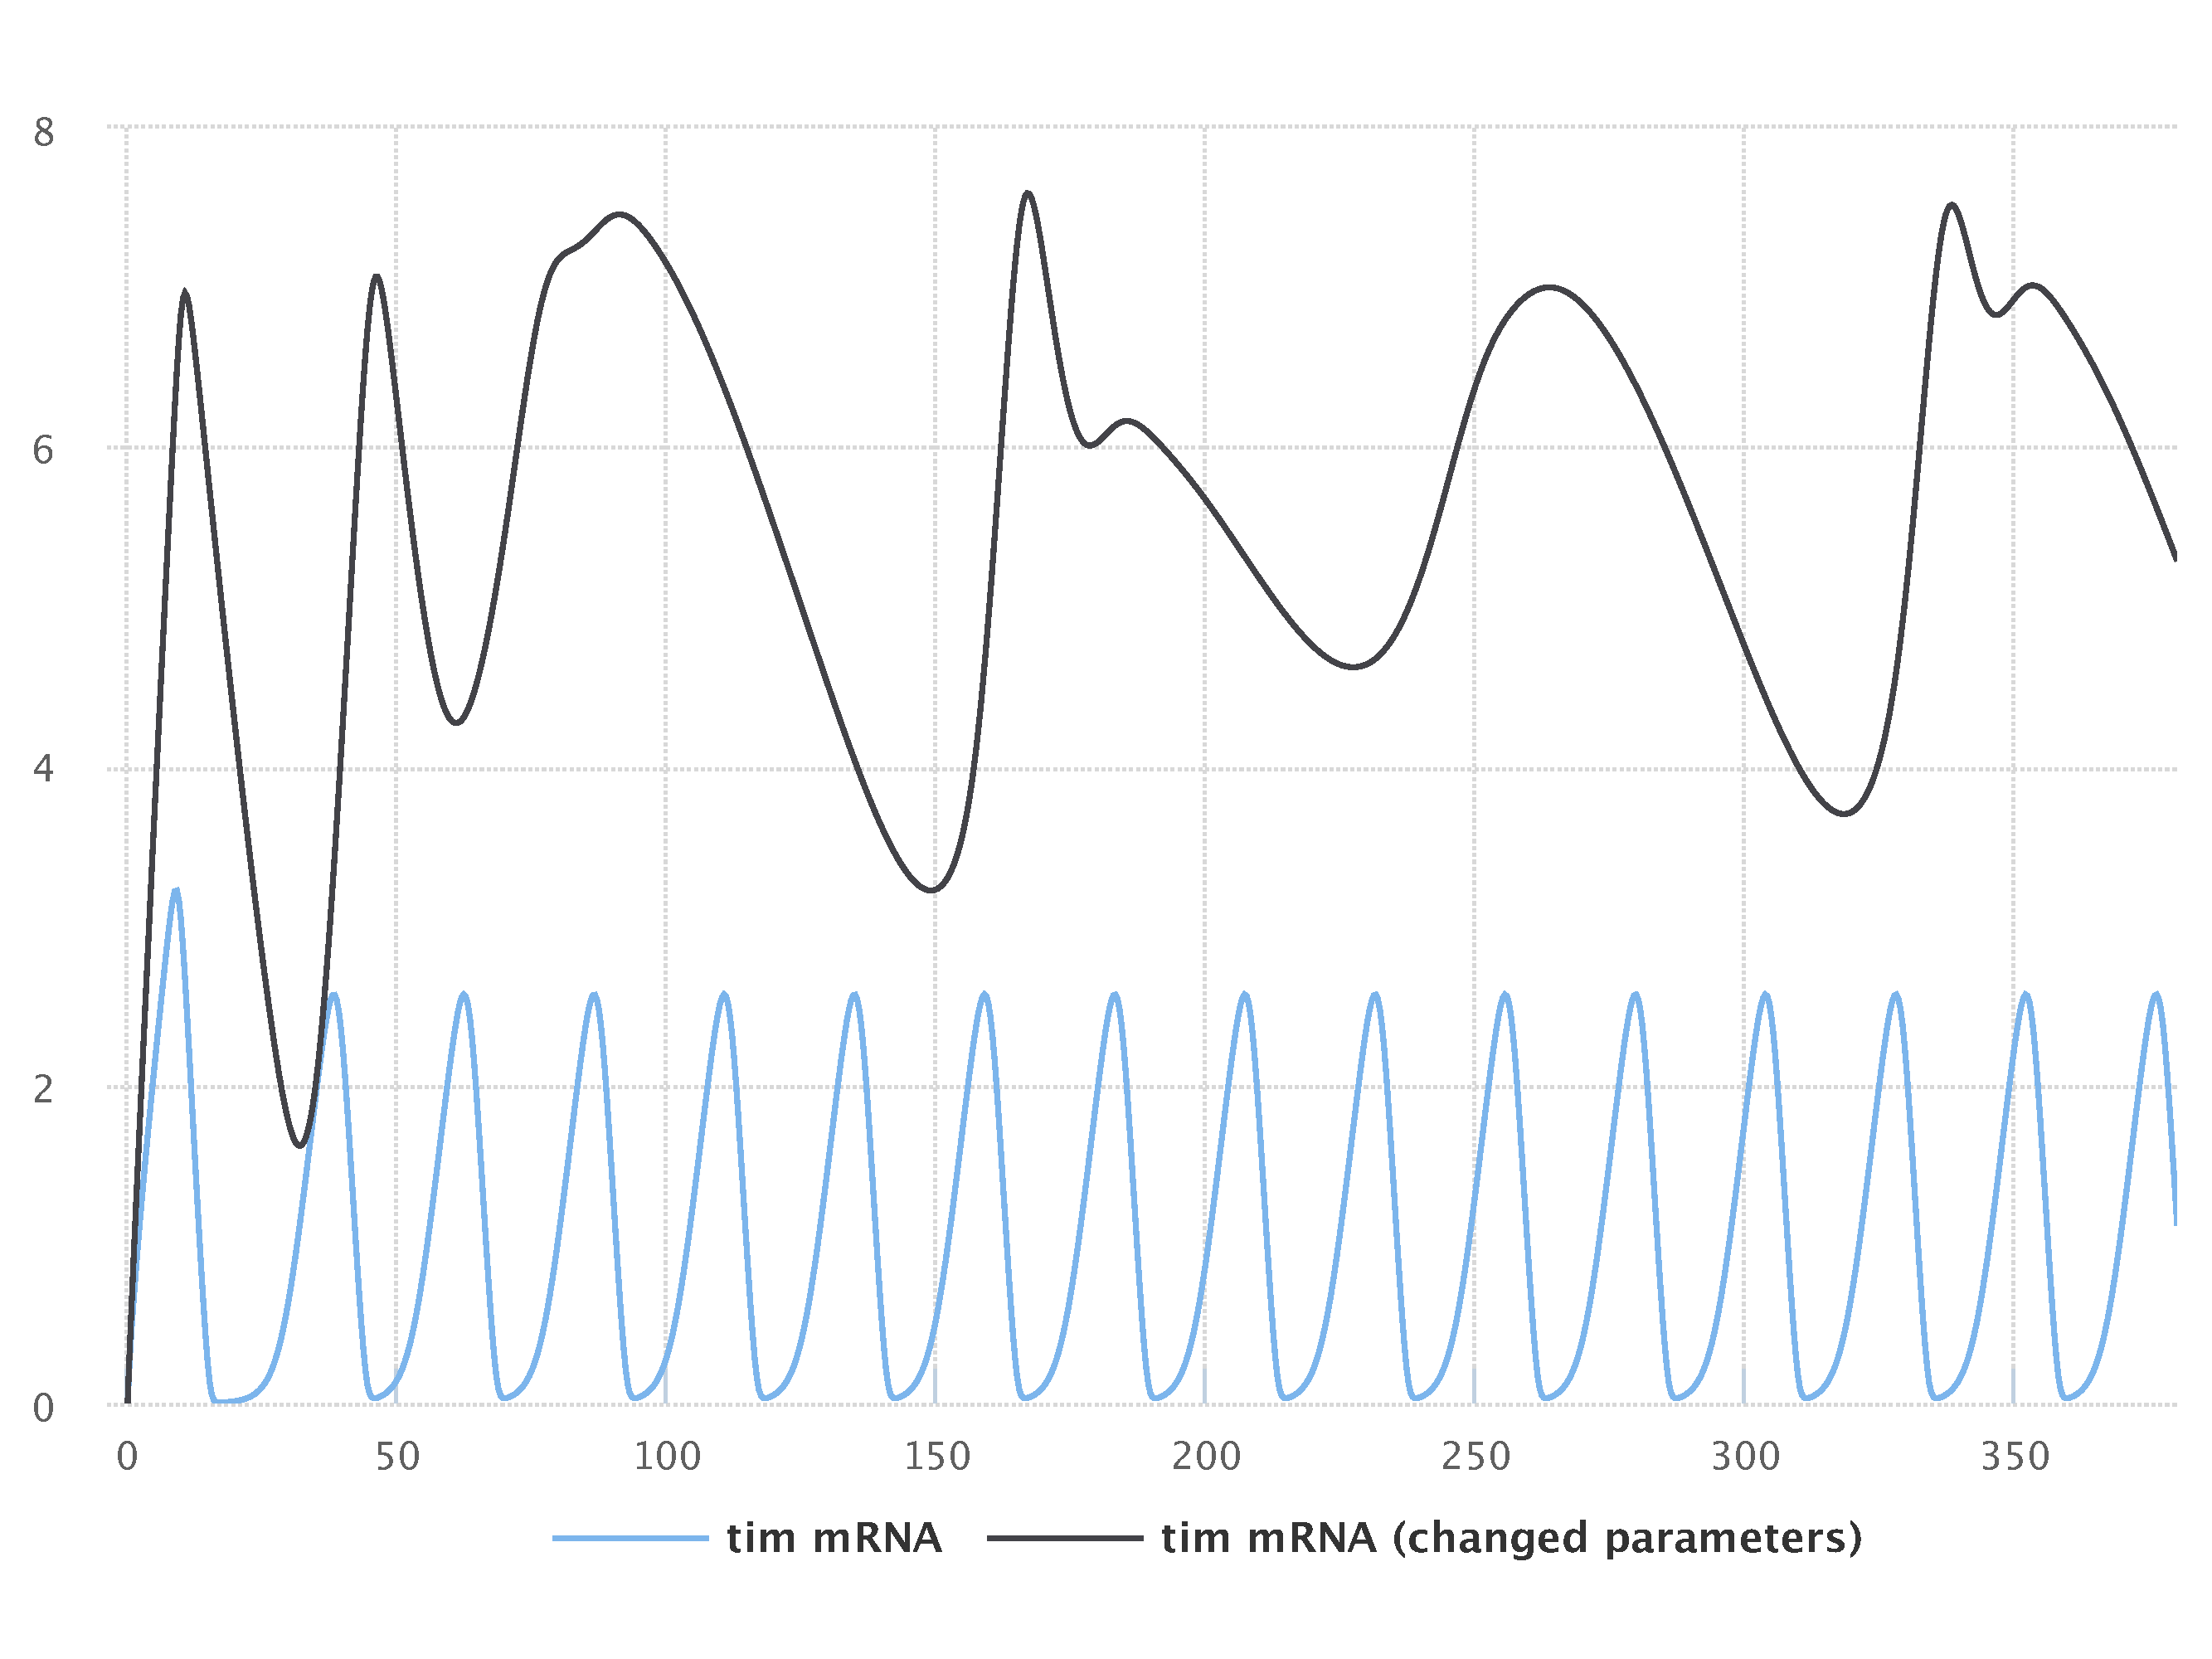
\includegraphics[width=1.0\textwidth]{examples/leloup-sbml/results/sedml_webtools/plot1}
		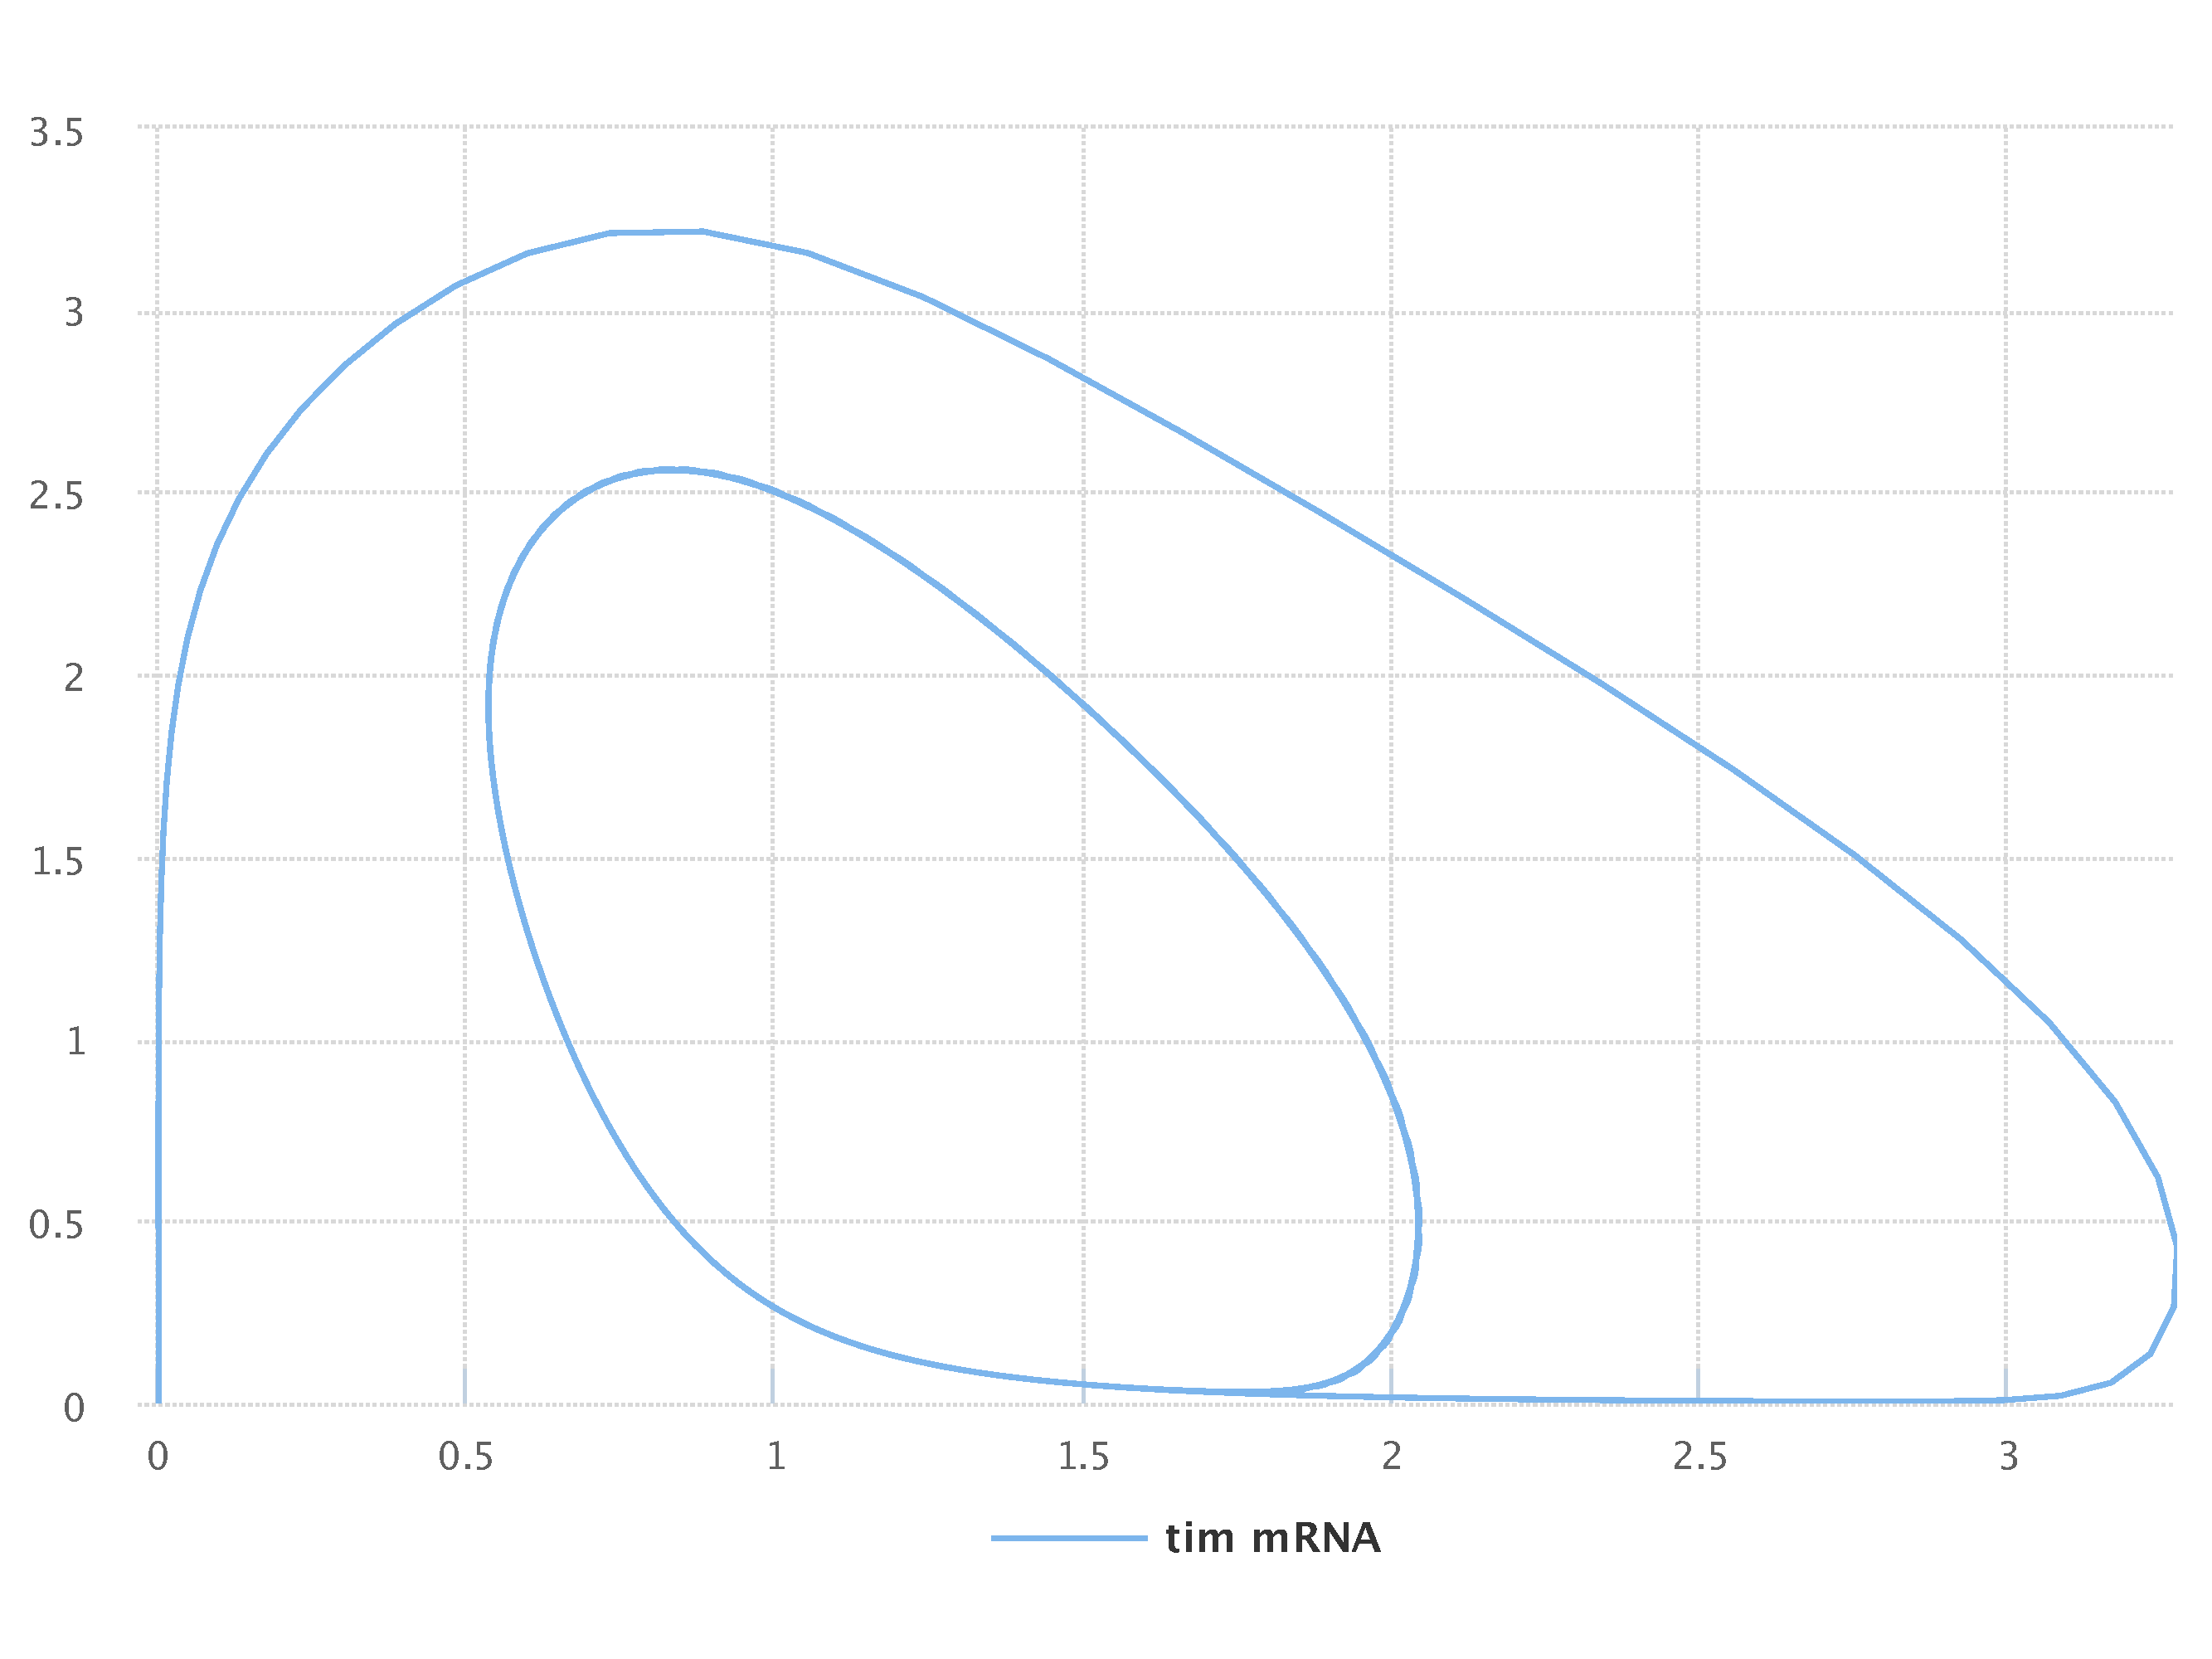
\includegraphics[width=1.0\textwidth]{examples/leloup-sbml/results/sedml_webtools/plot2}
		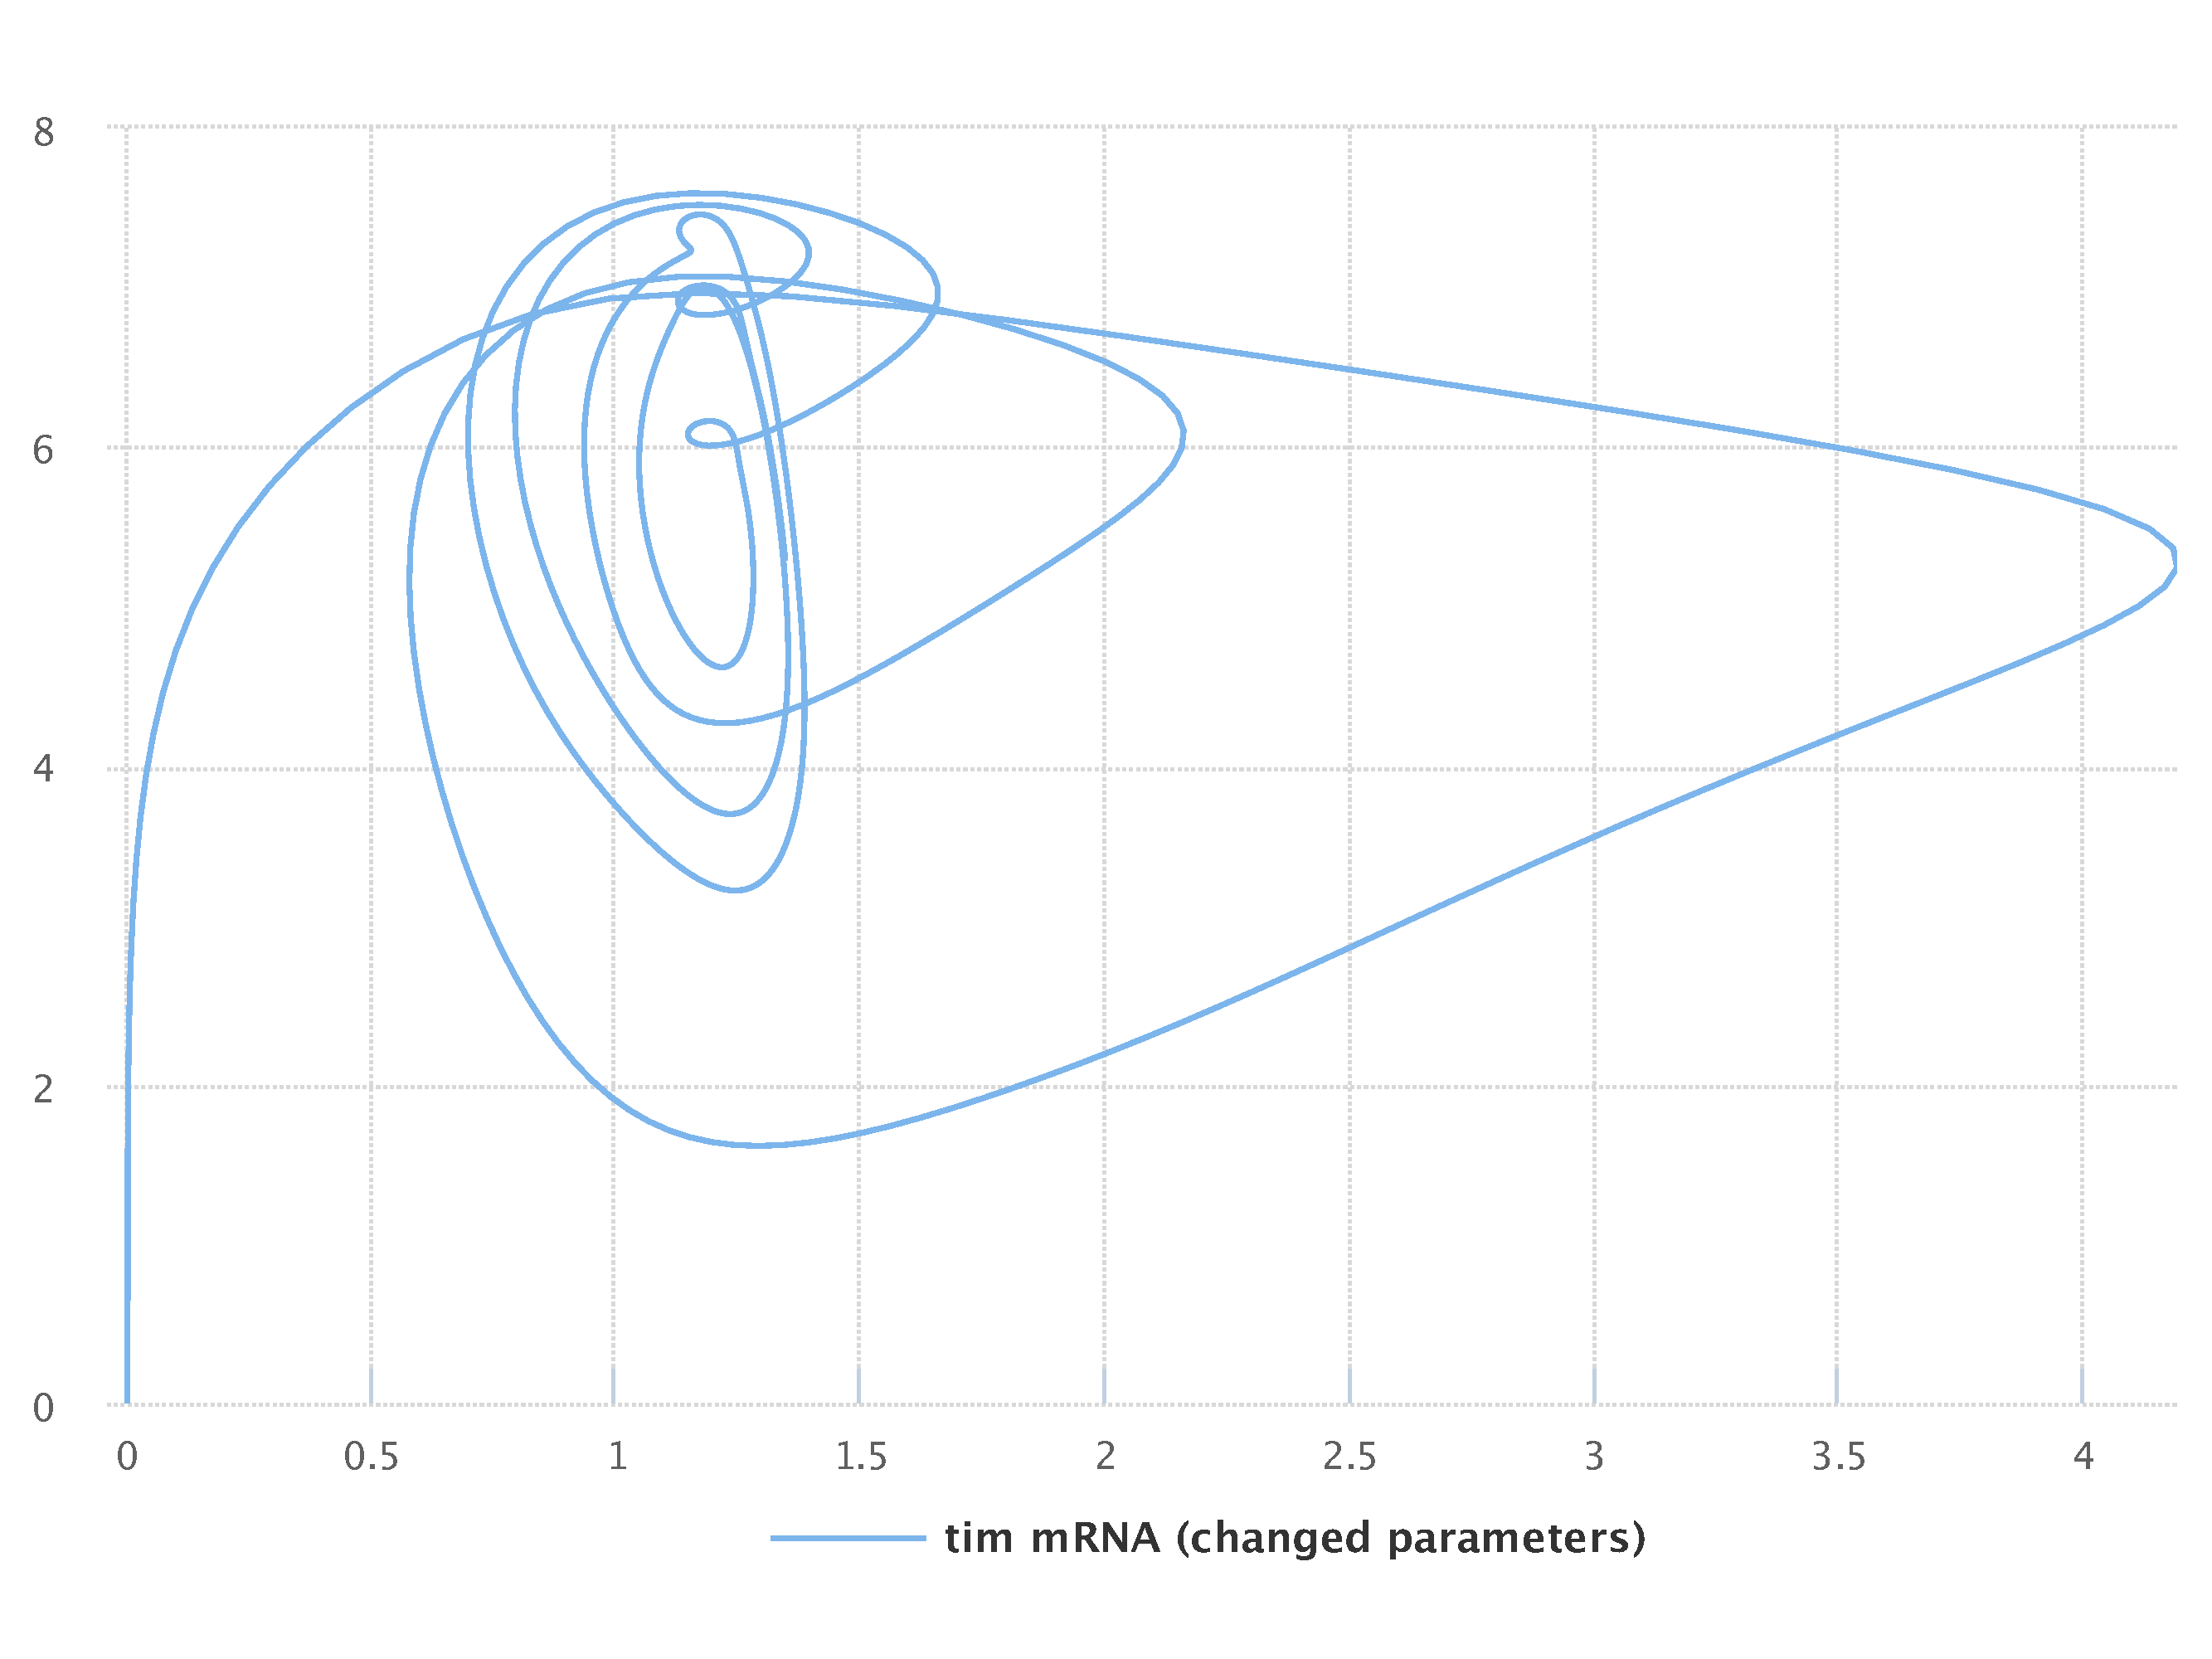
\includegraphics[width=1.0\textwidth]{examples/leloup-sbml/results/sedml_webtools/plot3}
        \caption{The simulation result gained from the simulation description given in \lst{leloup-sbml}. Simulation with SED-ML web tools \citep{bergmann2017sed}.}
        \label{fig:leloup-sbml1}
    \end{minipage}\hfill
    \begin{minipage}{0.47\textwidth}
        \centering
         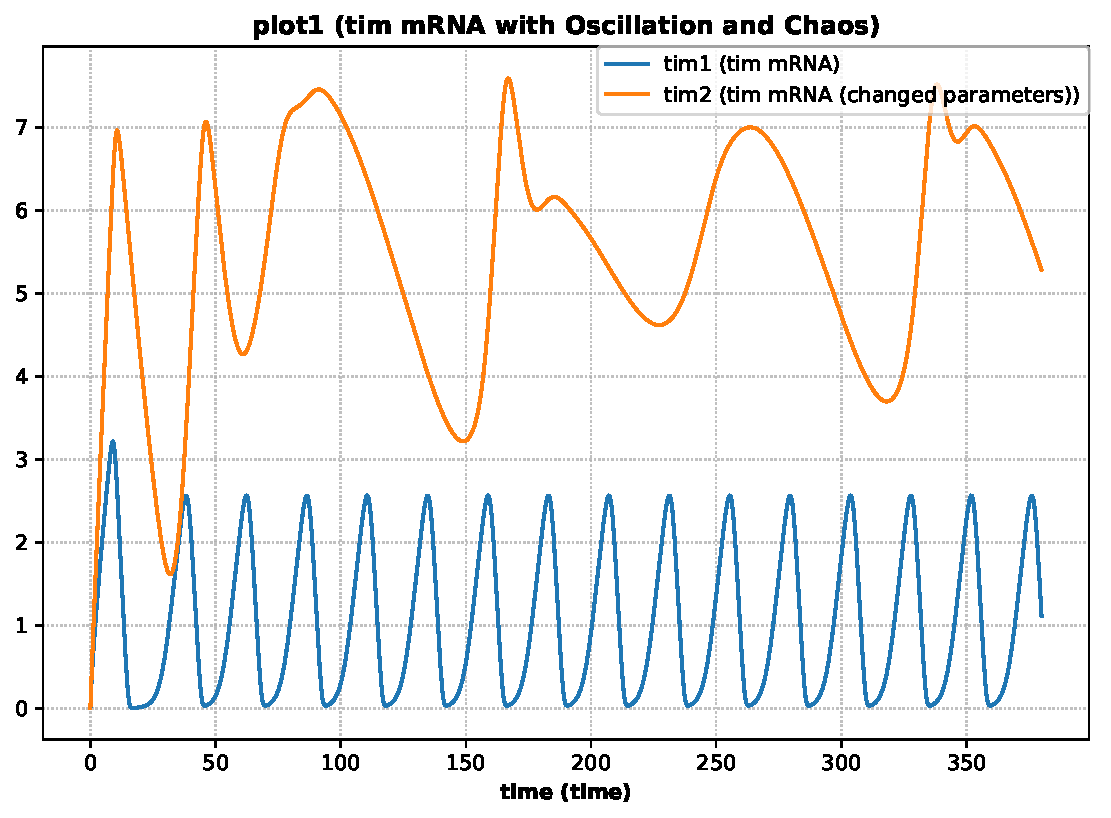
\includegraphics[width=1.0\textwidth]{examples/leloup-sbml/results/tellurium/plot1}
		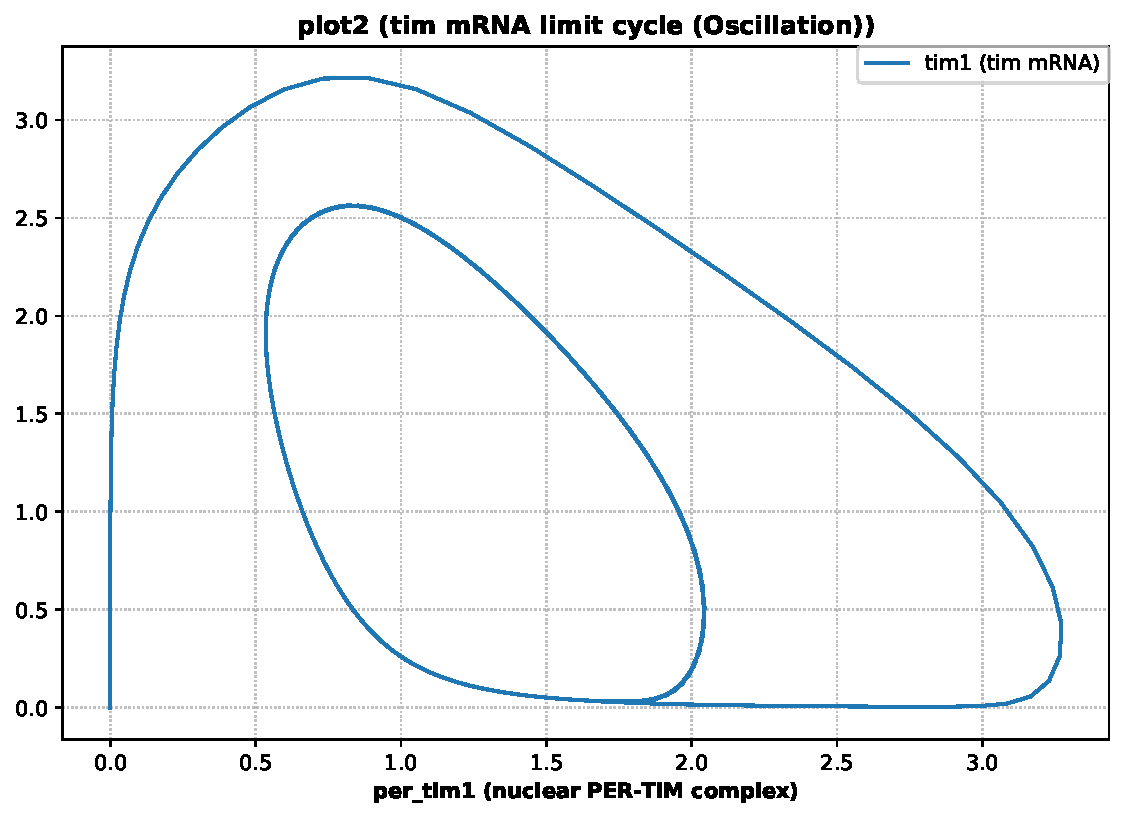
\includegraphics[width=1.0\textwidth]{examples/leloup-sbml/results/tellurium/plot2}
		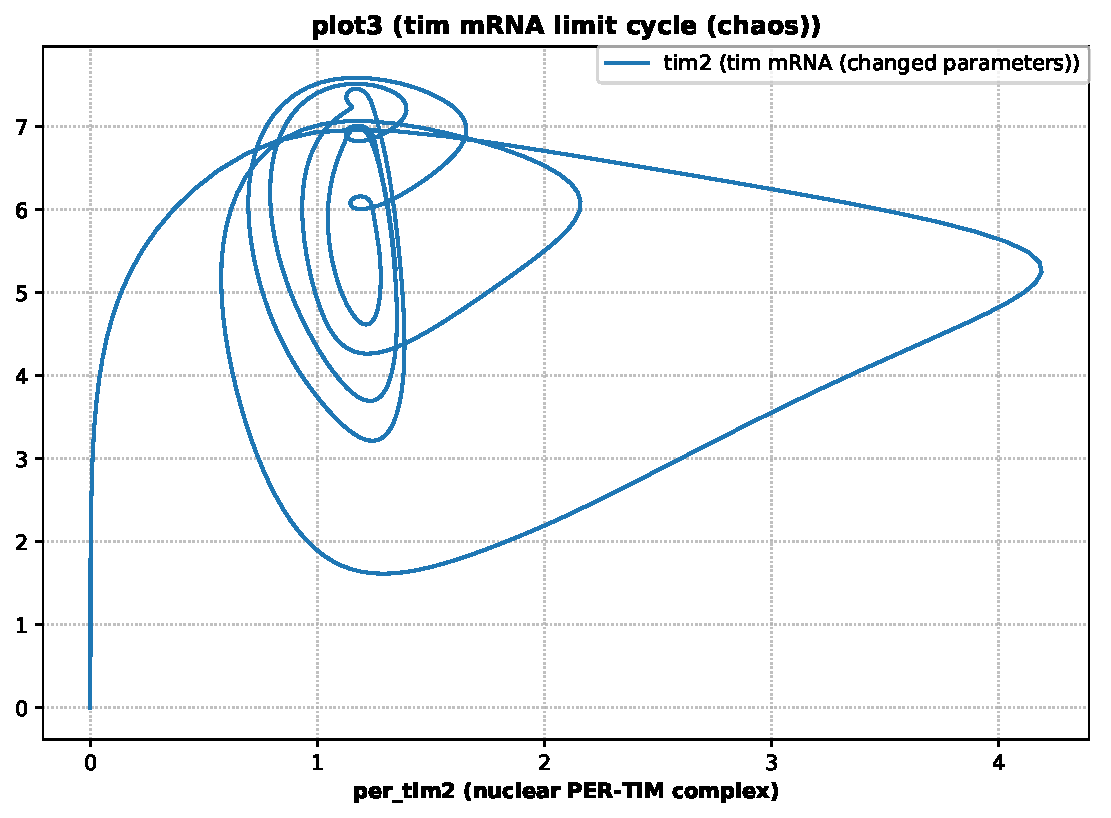
\includegraphics[width=1.0\textwidth]{examples/leloup-sbml/results/tellurium/plot3}
        \caption{Simulation with tellurium \citep{tellurium}.}
        \label{fig:leloup-sbml2}
    \end{minipage}
    
\end{figure}

\myXmlImport{LeLoup Model Simulation Description in SED-ML}{lst:leloup-sbml}{examples/leloup-sbml/leloup-sbml.xml}


% ~~~ IKAPPAB ~~~
\subsection{IkappaB signaling (\texttt{L1V3\_ikkapab.omex})}
The following example provides a SED-ML description for the simulation of the IkappaB-NF-kappaB signaling module described in \citep{hoffmann2002ikappab}.

This model is referenced by its SED-ML ID \code{model1} and refers to the model with the URL \url{https://www.ebi.ac.uk/biomodels/model/download/BIOMD0000000140.2?filename=BIOMD0000000140_url.xml}.

The simulation description specifies one simulation \code{simulation1}, which is a uniform timecourse simulation that simulates the model for 41 hours. \code{task1} then applies this simulation to the model.

As output this simulation description collects four parameters: \code{Total\_NFkBn}, \code{Total\_IkBbeta}, \code{Total\_IkBeps} and \code{Total\_IkBalpha}. These variables are plotted against the simulation time as shown in Figure \ref{fig:ikappab1} and \ref{fig:ikappab2}.  \changed{This document can be found at \url{https://sed-ml.org/examples/L1V3/L1V3_ikappab/ikappab.xml}, and an OMEX version at \url{https://sed-ml.org/examples/L1V3/L1V3_ikappab.omex}.}

\begin{figure}[ht]
    \centering
    \begin{minipage}{0.47\textwidth}
        \centering
        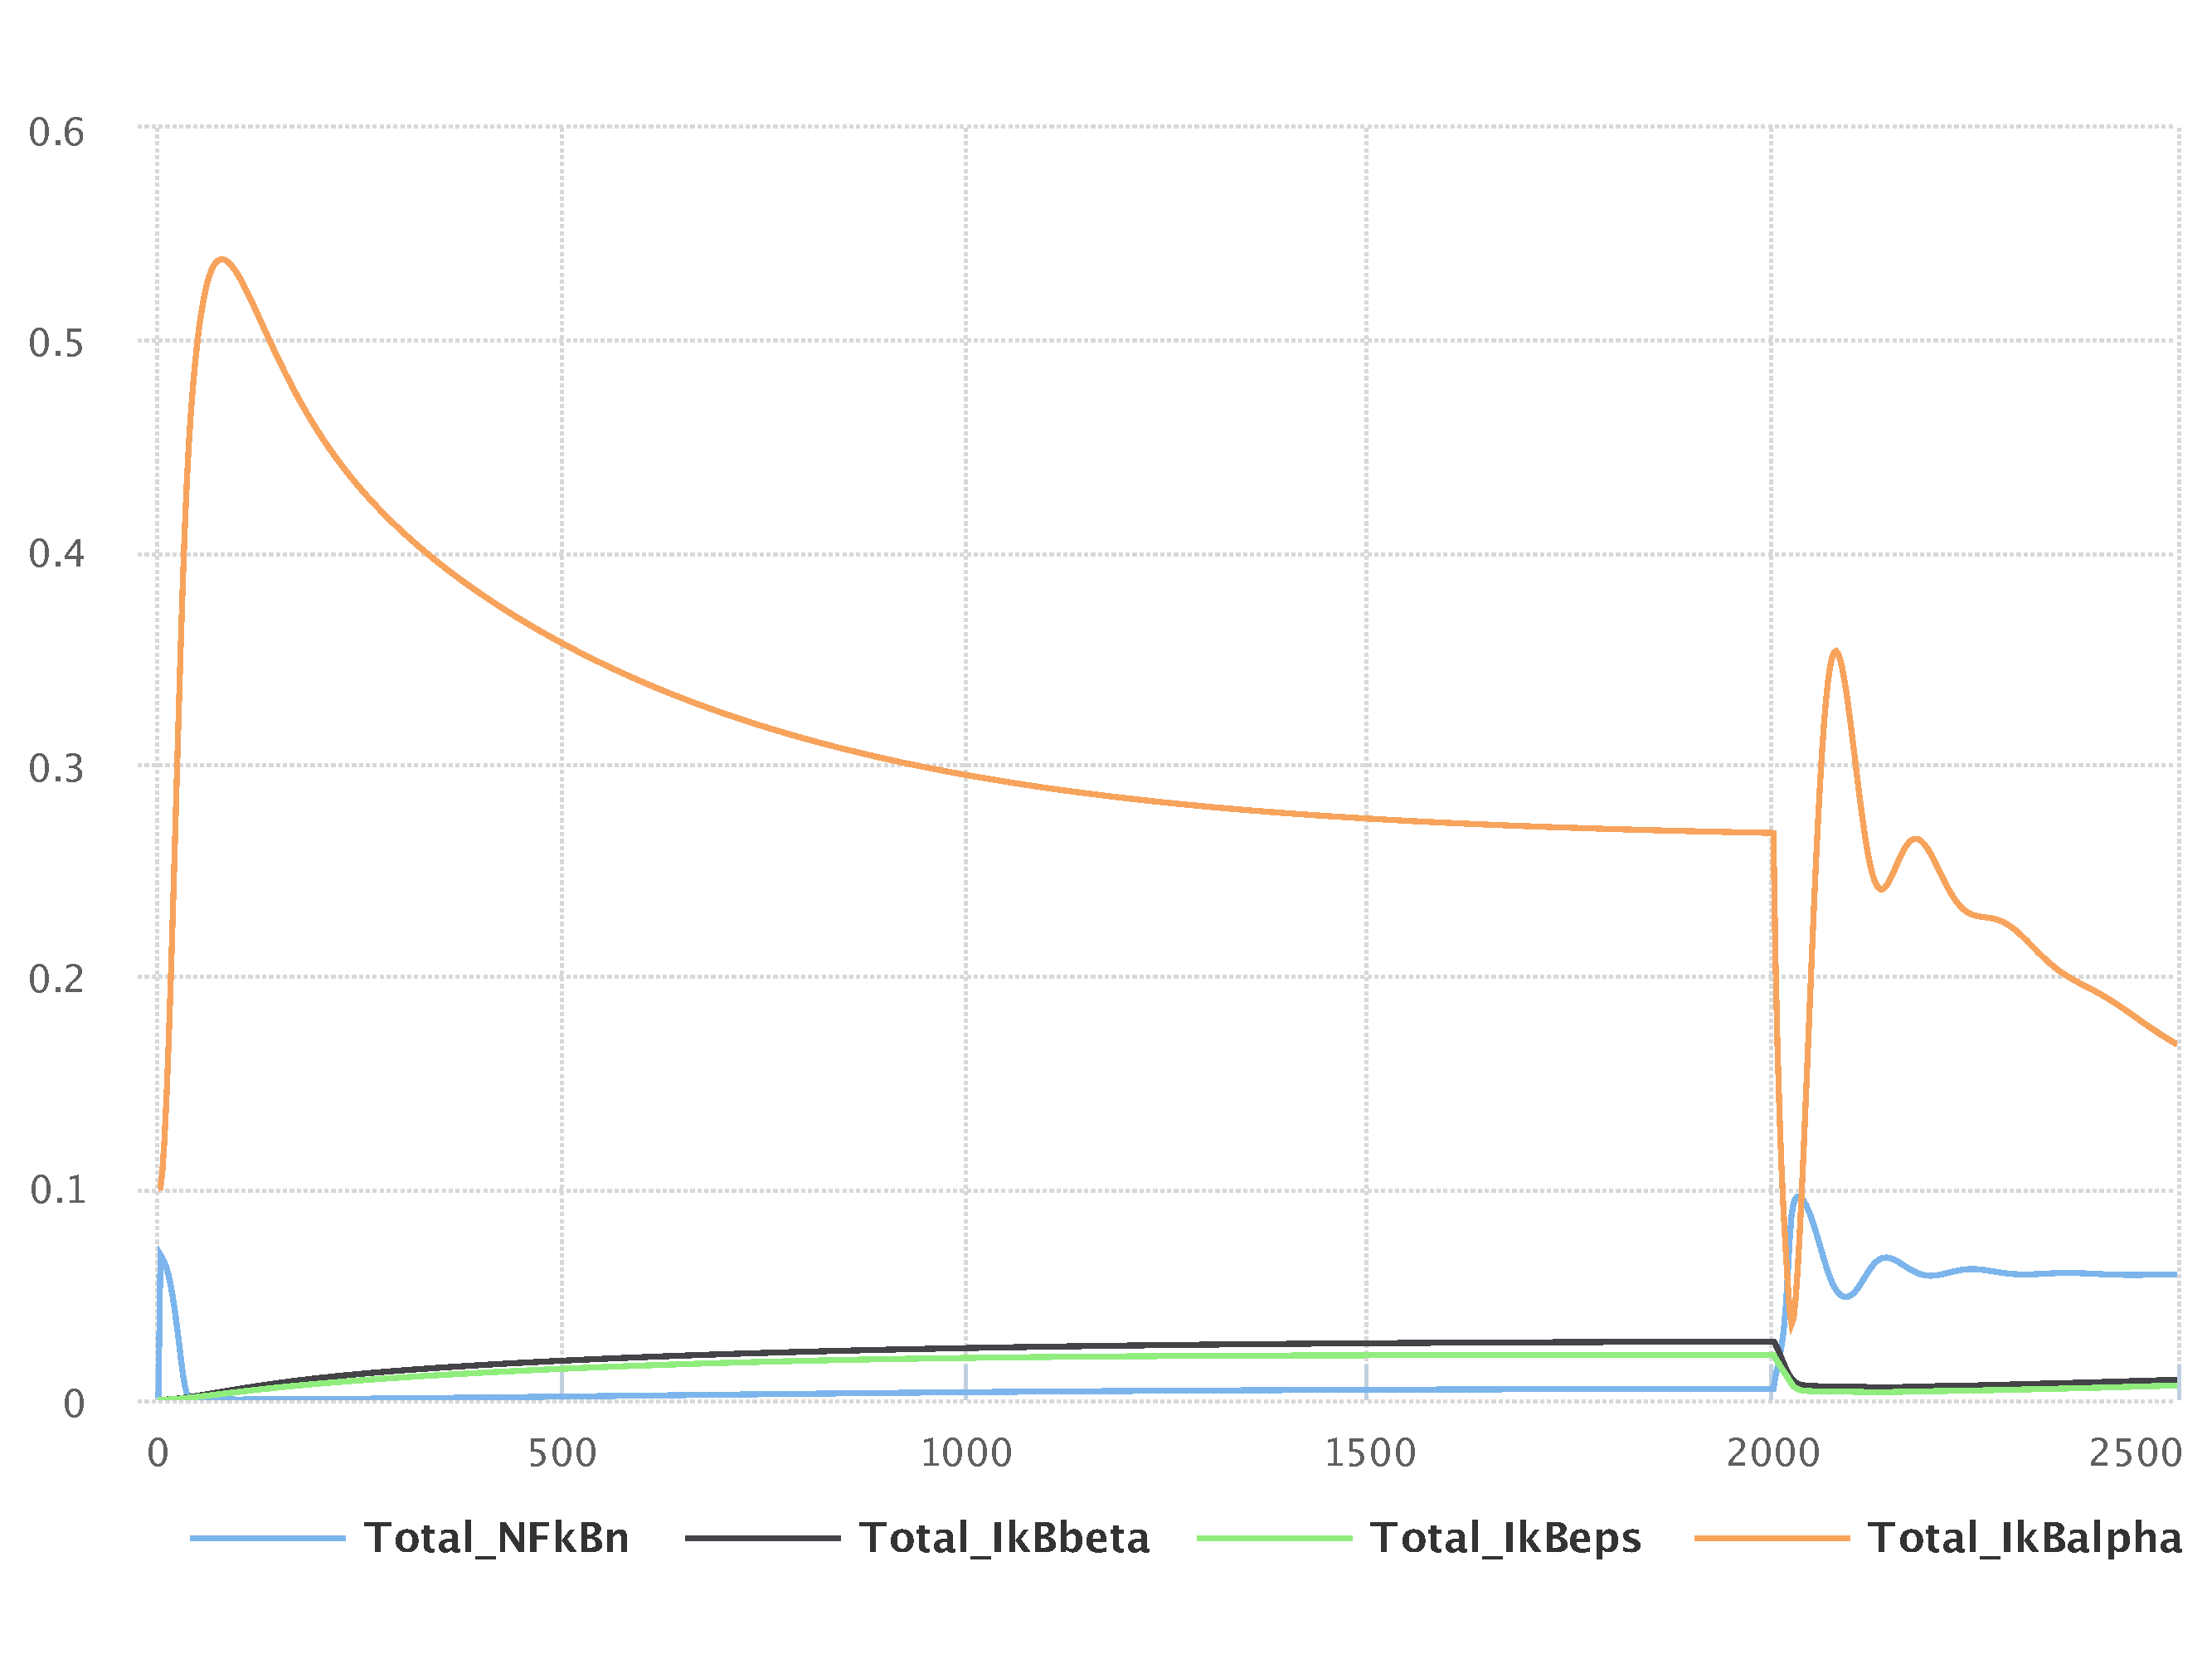
\includegraphics[width=1.0\textwidth]{examples/ikappab/results/sedml_webtools/plot1}
        \caption{The simulation result gained from the simulation description given in \lst{ikappab}. Simulation with SED-ML web tools \citep{bergmann2017sed}.}
        \label{fig:ikappab1}
    \end{minipage}\hfill
    \begin{minipage}{0.47\textwidth}
        \centering
        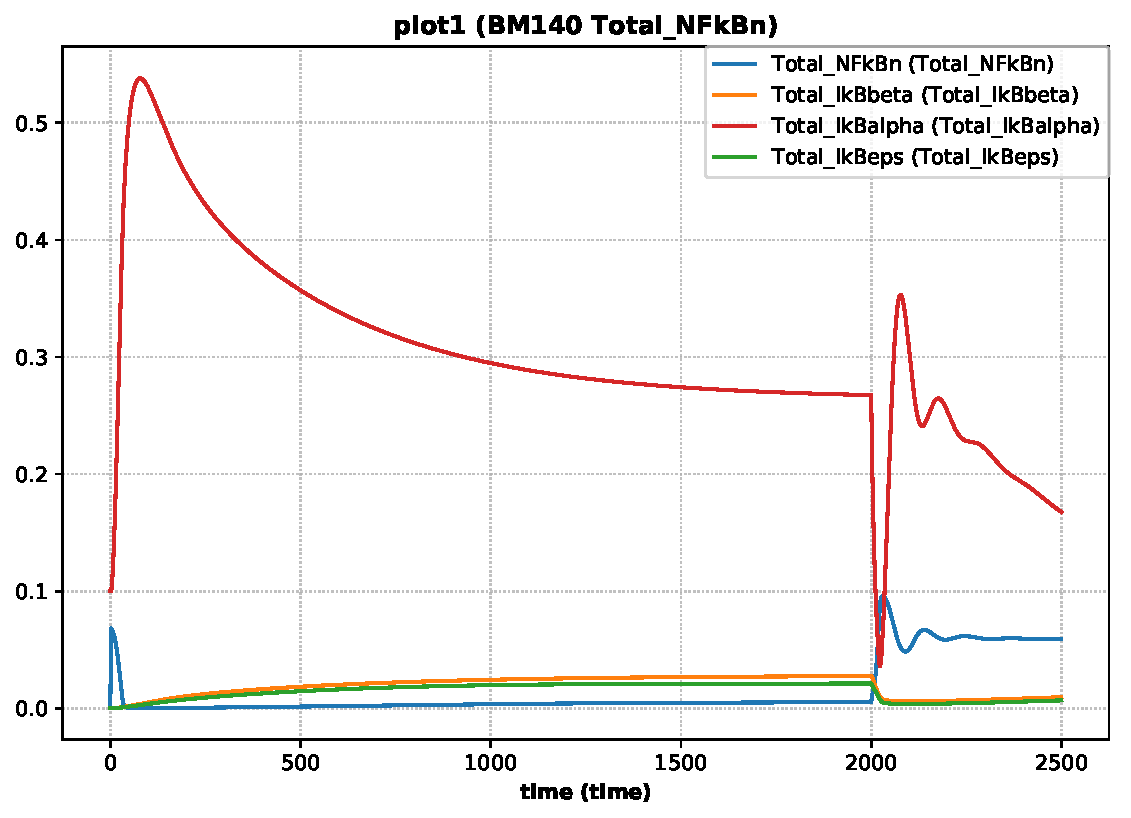
\includegraphics[width=1.0\textwidth]{examples/ikappab/results/tellurium/plot1}
        \caption{Simulation with tellurium \citep{tellurium}.}
        \label{fig:ikappab2}
    \end{minipage}
\end{figure}

\myXmlImport{IkappaB-NF-kappaB signaling Model Simulation Description in SED-ML}{lst:ikappab}{examples/ikappab/ikappab.xml}
